% Manual de usuario de EmprendeU. Compilar con pdfLaTeX (dos pasadas): pdflatex manual_usuario.tex
\documentclass[12pt,letterpaper]{article}
\usepackage[utf8]{inputenc}
\usepackage[T1]{fontenc}
\usepackage{tgtermes}                 % Times New Roman (clon metrico, paquete texlive-tex-gyre)
\usepackage[spanish,es-noshorthands]{babel}
\addto\captionsspanish{%
  \renewcommand{\tablename}{Tabla}%
  \renewcommand{\listtablename}{ÍNDICE DE TABLAS}%
  \renewcommand{\listfigurename}{ÍNDICE DE FIGURAS}%
  \renewcommand{\contentsname}{ÍNDICE GENERAL}%
}
\usepackage[letterpaper,margin=2.54cm]{geometry}
\usepackage{etoolbox}
\usepackage{setspace}
\usepackage{indentfirst}
\usepackage{graphicx}
\usepackage{float}
\usepackage{booktabs}
\usepackage{tabularx}
\usepackage{enumitem}
\usepackage{caption}
\usepackage{titlesec}
\usepackage{tocloft}
\usepackage{fancyhdr}
\usepackage[hidelinks]{hyperref}

\setlength{\parindent}{1.27cm}
\setlength{\parskip}{0pt}
\raggedright
\setlist{itemsep=2pt,topsep=4pt,parsep=0pt}
\setlist[enumerate,itemize]{leftmargin=1.27cm}

% Encabezado APA: número de página arriba a la derecha
\fancypagestyle{apa}{\fancyhf{}\fancyhead[R]{\thepage}\renewcommand{\headrulewidth}{0pt}}
\setlength{\headheight}{14.5pt}

% Títulos (niveles APA 1 a 3)
\titleformat{\section}{\normalfont\bfseries\centering}{}{0pt}{}
\titleformat{\subsection}{\normalfont\bfseries\raggedright}{}{0pt}{}
\titleformat{\subsubsection}{\normalfont\bfseries\itshape\raggedright}{}{0pt}{}
\titlespacing*{\section}{0pt}{0pt}{0pt}
\titlespacing*{\subsection}{0pt}{0pt}{0pt}
\titlespacing*{\subsubsection}{0pt}{0pt}{0pt}

% Figuras y tablas: «Figura N» en negrita, título en cursiva en la línea siguiente
\captionsetup{labelsep=newline,labelfont=bf,textfont=it,justification=raggedright,singlelinecheck=off,skip=4pt}
\captionsetup[table]{position=top}

% Índices con la misma sangría jerárquica
\renewcommand{\cftsecfont}{\bfseries}
\setlength{\cftsubsecindent}{1.27cm}
\setlength{\cftsubsubsecindent}{2.54cm}
\renewcommand{\cftfigpresnum}{Figura\ }
\renewcommand{\cfttabpresnum}{Tabla\ }
\setlength{\cftfignumwidth}{2.2cm}\setlength{\cfttabnumwidth}{2cm}
\setlength{\cftsecnumwidth}{0pt}\setlength{\cftsubsecnumwidth}{0pt}\setlength{\cftsubsubsecnumwidth}{0pt}
\renewcommand{\cftdot}{.}
\renewcommand{\cftsecleader}{\cftdotfill{\cftdotsep}}
\setcounter{tocdepth}{3}

% Referencias con sangría francesa
\newenvironment{hangref}{\par\singlespacing\setlength{\parindent}{-1.27cm}\setlength{\leftskip}{1.27cm}}{\par}

% Listas y tablas a interlineado sencillo; el texto corrido, doble
\AtBeginEnvironment{enumerate}{\singlespacing}
\AtBeginEnvironment{itemize}{\singlespacing}
\sloppy

\begin{document}

\begin{titlepage}\thispagestyle{empty}\centering\singlespacing
{\bfseries Centro de Innovación y Emprendimiento Universitario (CIE-U)\par}\vspace{2.5cm}
{\fontsize{30}{36}\selectfont\bfseries EmprendeU\par}\vspace{.4cm}
{\itshape Plataforma universitaria de emprendimiento\par}\vspace{2cm}
{\fontsize{22}{26}\selectfont\bfseries MANUAL DE USUARIO\par}\vspace{.6cm}
Panel web del personal del CIE-U y aplicación móvil del emprendedor\par\vspace{2.5cm}
Versión 1.0\par\vspace{.4cm}Equipo responsable: Equipo de desarrollo de EmprendeU (por confirmar)\par\vspace{.4cm}18 de noviembre de 2026\par
\end{titlepage}
\pagestyle{apa}\setcounter{page}{2}
\clearpage
\tableofcontents\clearpage
\listoffigures\clearpage
\listoftables\clearpage
\doublespacing

\clearpage

\section*{CAPÍTULO 1. INTRODUCCIÓN}

\addcontentsline{toc}{section}{CAPÍTULO 1. INTRODUCCIÓN}

\subsection*{1.1. Presentación del sistema}

\addcontentsline{toc}{subsection}{1.1. Presentación del sistema}

EmprendeU es la plataforma universitaria de emprendimiento del Centro de Innovación y Emprendimiento Universitario (CIE-U). Reúne en un mismo sistema el acompañamiento a los emprendimientos de estudiantes: seguimiento de etapas, mentorías con asesores, retos con puntos de experiencia (XP), capacitaciones, alertas de riesgo y un coach de inteligencia artificial.

El sistema se compone de dos aplicaciones que comparten los mismos datos. El \textbf{panel web} lo utiliza el personal del CIE-U (administradores, coordinadores y asesores). La \textbf{aplicación móvil} la utilizan las personas emprendedoras.

\subsection*{1.2. Objetivo del manual}

\addcontentsline{toc}{subsection}{1.2. Objetivo del manual}

Este manual explica, paso a paso, cómo utilizar las funciones disponibles de EmprendeU, desde la perspectiva de la persona usuaria y sin requerir conocimientos de programación.

\subsection*{1.3. Alcance del documento}

\addcontentsline{toc}{subsection}{1.3. Alcance del documento}

El manual documenta las funcionalidades implementadas y comprobadas en la versión analizada del sistema: el panel web (rutas públicas y rutas del personal) y la aplicación móvil del emprendedor. No describe funciones planificadas que no estén implementadas. Los aspectos que no pudieron comprobarse se indican como \textit{pendientes de verificación} y se listan en el Anexo B.

\subsection*{1.4. Público al que está dirigido}

\addcontentsline{toc}{subsection}{1.4. Público al que está dirigido}

\begin{itemize}
\item Personal administrador, coordinador y asesor del CIE-U, que usa el panel web.
\item Estudiantes emprendedores, que usan la aplicación móvil y pueden postular desde la web pública.
\end{itemize}

\subsection*{1.5. Descripción general del sistema}

\addcontentsline{toc}{subsection}{1.5. Descripción general del sistema}

Los emprendimientos avanzan por cuatro etapas: Preincubación, Incubación, Crecimiento y Graduación. En cada etapa, el emprendedor cumple retos que otorgan XP e insignias. Los asesores acompañan con mentorías, recomendaciones y compromisos. La coordinación supervisa la salud de cada emprendimiento mediante indicadores, alertas y reportes.

\subsection*{1.6. Organización del manual}

\addcontentsline{toc}{subsection}{1.6. Organización del manual}

El Capítulo 2 describe el sistema y sus roles. El Capítulo 3 explica el acceso. El Capítulo 4 presenta la interfaz. El Capítulo 5 detalla cada módulo. El Capítulo 6 reúne procedimientos completos. Los Capítulos 7 a 10 tratan los mensajes y la solución de problemas, las buenas prácticas, el glosario y las preguntas frecuentes.

\clearpage

\section*{CAPÍTULO 2. INFORMACIÓN GENERAL DEL SISTEMA}

\addcontentsline{toc}{section}{CAPÍTULO 2. INFORMACIÓN GENERAL DEL SISTEMA}

\subsection*{2.1. Descripción del software}

\addcontentsline{toc}{subsection}{2.1. Descripción del software}

EmprendeU es una solución multiplataforma. El panel web funciona en un navegador actual. La aplicación móvil está desarrollada para Android e iOS; en la verificación de este manual se ejecutó en un teléfono Android.

\subsection*{2.2. Características principales}

\addcontentsline{toc}{subsection}{2.2. Características principales}

\begin{itemize}
\item Postulación pública de emprendimientos y admisión por parte del CIE-U.
\item Registro de emprendedores y emprendimientos, con equipo y etapas.
\item Mentorías: asignación de asesores, disponibilidad horaria y registro de sesiones.
\item Retos, XP, niveles e insignias para el emprendedor.
\item Alertas de riesgo, indicadores de salud y reportes exportables (CSV y Excel).
\item Capacitaciones con inscripción y asistencia.
\item Coach de IA para el emprendedor, que también funciona sin internet si se descarga la IA en el teléfono.
\item Asistente de ayuda y tutorial guiado en el panel web.
\item Notificaciones dentro de la aplicación móvil.
\end{itemize}

\subsection*{2.3. Requisitos para su utilización}

\addcontentsline{toc}{subsection}{2.3. Requisitos para su utilización}

\begin{itemize}
\item \textbf{Panel web:} navegador actual y una cuenta creada por el CIE-U con rol de personal.
\item \textbf{Aplicación móvil:} teléfono con la aplicación instalada y una cuenta de emprendedor. Casi todas las funciones requieren conexión a internet.
\item \textbf{IA sin conexión (opcional):} dispositivo Android compatible. Se descargan aproximadamente 2,6 GB y 165 MB, por lo que se recomienda usar Wi-Fi y disponer del doble del tamaño libre.
\end{itemize}

\subsection*{2.4. Roles de usuario}

\addcontentsline{toc}{subsection}{2.4. Roles de usuario}

\begin{table}[H]\singlespacing\small
\caption{Roles del sistema}
\begin{tabularx}{\textwidth}{XXX}
\toprule
\textbf{Rol} & \textbf{Dónde trabaja} & \textbf{Descripción} \\
\midrule
\relax Administrador & Panel web & Gestiona usuarios, roles, permisos, parámetros y catálogos. \\
\relax Coordinador & Panel web & Supervisa emprendedores, emprendimientos, mentorías, alertas y reportes. \\
\relax Asesor / Mentor & Panel web & Acompaña a los emprendimientos que tiene asignados. \\
\relax Emprendedor & Aplicación móvil & Gestiona su emprendimiento, sus retos y sus mentorías. \\
\bottomrule
\end{tabularx}
\end{table}

El panel web rechaza las cuentas de emprendedor con el mensaje «Esta cuenta es de emprendedor: usa la app móvil del CIE-U.». La aplicación móvil rechaza las cuentas del personal con «Esta cuenta es del panel web del CIE-U. Esta app es para emprendedores.». Un administrador puede crear roles personalizados y editar los permisos de cada rol, por lo que la tabla siguiente muestra la configuración inicial.

\subsection*{2.5. Funcionalidades disponibles por rol}

\addcontentsline{toc}{subsection}{2.5. Funcionalidades disponibles por rol}

Los permisos se agrupan en siete módulos y cuatro acciones: consulta (C), registro (R), modificación (M) y administrativo (A).

\begin{table}[H]\singlespacing\small
\caption{Permisos iniciales por rol}
\begin{tabularx}{\textwidth}{XXXXX}
\toprule
\textbf{Módulo} & \textbf{Administrador} & \textbf{Coordinador} & \textbf{Asesor} & \textbf{Emprendedor} \\
\midrule
\relax Usuarios y roles & C R M A & — & — & — \\
\relax Emprendedores y emprendimientos & C & C R M & C & C R \\
\relax Asesorías y mentorías & C & C R & C R M & C \\
\relax Seguimiento y etapas & C & C R M & C R & C R \\
\relax Asistente inteligente & — & C & — & C R \\
\relax Indicadores y reportes & C & C R & — & — \\
\relax Configuración del sistema & C R M A & C M & — & — \\
\bottomrule
\end{tabularx}
\end{table}

El menú lateral muestra solo las pantallas permitidas por los permisos de la persona. Si una pantalla no está permitida, el sistema muestra «Sin acceso a \ldots{}» con el texto «Tu rol no tiene permiso para ver esta sección. Si lo necesitas, pídeselo a un administrador.».

\subsection*{2.6. Recomendaciones generales de utilización}

\addcontentsline{toc}{subsection}{2.6. Recomendaciones generales de utilización}

\begin{itemize}
\item Cierre la sesión al terminar, sobre todo en equipos compartidos.
\item Cambie la contraseña temporal que recibió al crearse su cuenta.
\item Revise los datos antes de confirmar acciones definitivas, como admitir o rechazar una postulación.
\end{itemize}

\clearpage

\section*{CAPÍTULO 3. ACCESO AL SISTEMA}

\addcontentsline{toc}{section}{CAPÍTULO 3. ACCESO AL SISTEMA}

\subsection*{3.1. Ingreso a la aplicación}

\addcontentsline{toc}{subsection}{3.1. Ingreso a la aplicación}

El panel web se abre desde el navegador, en la dirección que el CIE-U proporcione. La página de inicio (Figura~\ref{fig:web_landing}) presenta el programa y ofrece los botones «Postula tu emprendimiento» y «Personal CIE-U». Si ya hay una sesión activa, aparece «Ir al panel».

\begin{figure}[H]\singlespacing
\caption{Página de inicio del sistema}\label{fig:web_landing}
\centering\fbox{
\includegraphics[width=0.97\textwidth,keepaspectratio]{imagenes/web_landing.png}}
\par\vspace{3pt}\begin{flushleft}\small \textit{Nota.} Página pública dirigida a estudiantes. «Personal CIE-U» lleva al inicio de sesión.\end{flushleft}
\end{figure}

\subsection*{3.2. Inicio de sesión}

\addcontentsline{toc}{subsection}{3.2. Inicio de sesión}

\textbf{Panel web.}

\begin{enumerate}
\item En la página de inicio, seleccionar «Personal CIE-U».
\item Escribir el «Correo electrónico».
\item Escribir la «Contraseña».
\item Seleccionar «Ingresar al panel».
\item El sistema abre la pantalla «Resumen».
\end{enumerate}

\begin{figure}[H]\singlespacing
\caption{Inicio de sesión del panel web}\label{fig:web_login}
\centering\fbox{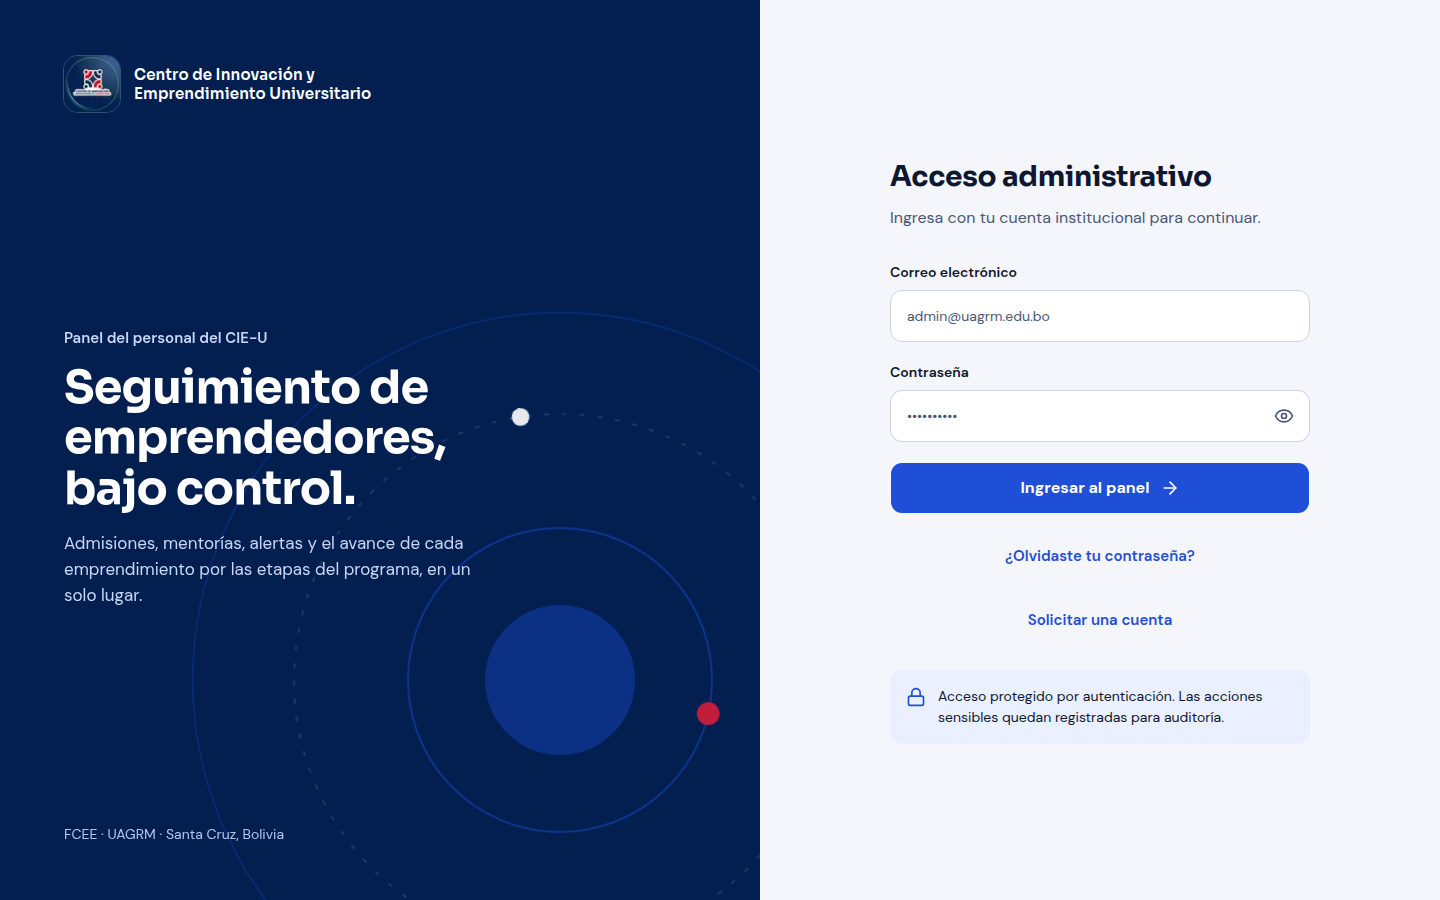
\includegraphics[width=0.97\textwidth,keepaspectratio]{imagenes/web_login.png}}
\par\vspace{3pt}\begin{flushleft}\small \textit{Nota.} Pantalla «Panel del personal del CIE-U».\end{flushleft}
\end{figure}

\textbf{Aplicación móvil.}

\begin{enumerate}
\item Abrir la aplicación EmprendeU.
\item Escribir el «Correo electrónico» y la «Contraseña». El ícono del ojo muestra u oculta la contraseña.
\item Tocar «Ingresar».
\item La aplicación abre la pantalla «Inicio».
\end{enumerate}

\begin{figure}[H]\singlespacing
\caption{Inicio de sesión de la aplicación móvil con un mensaje de error}\label{fig:movil_login_error}
\centering\fbox{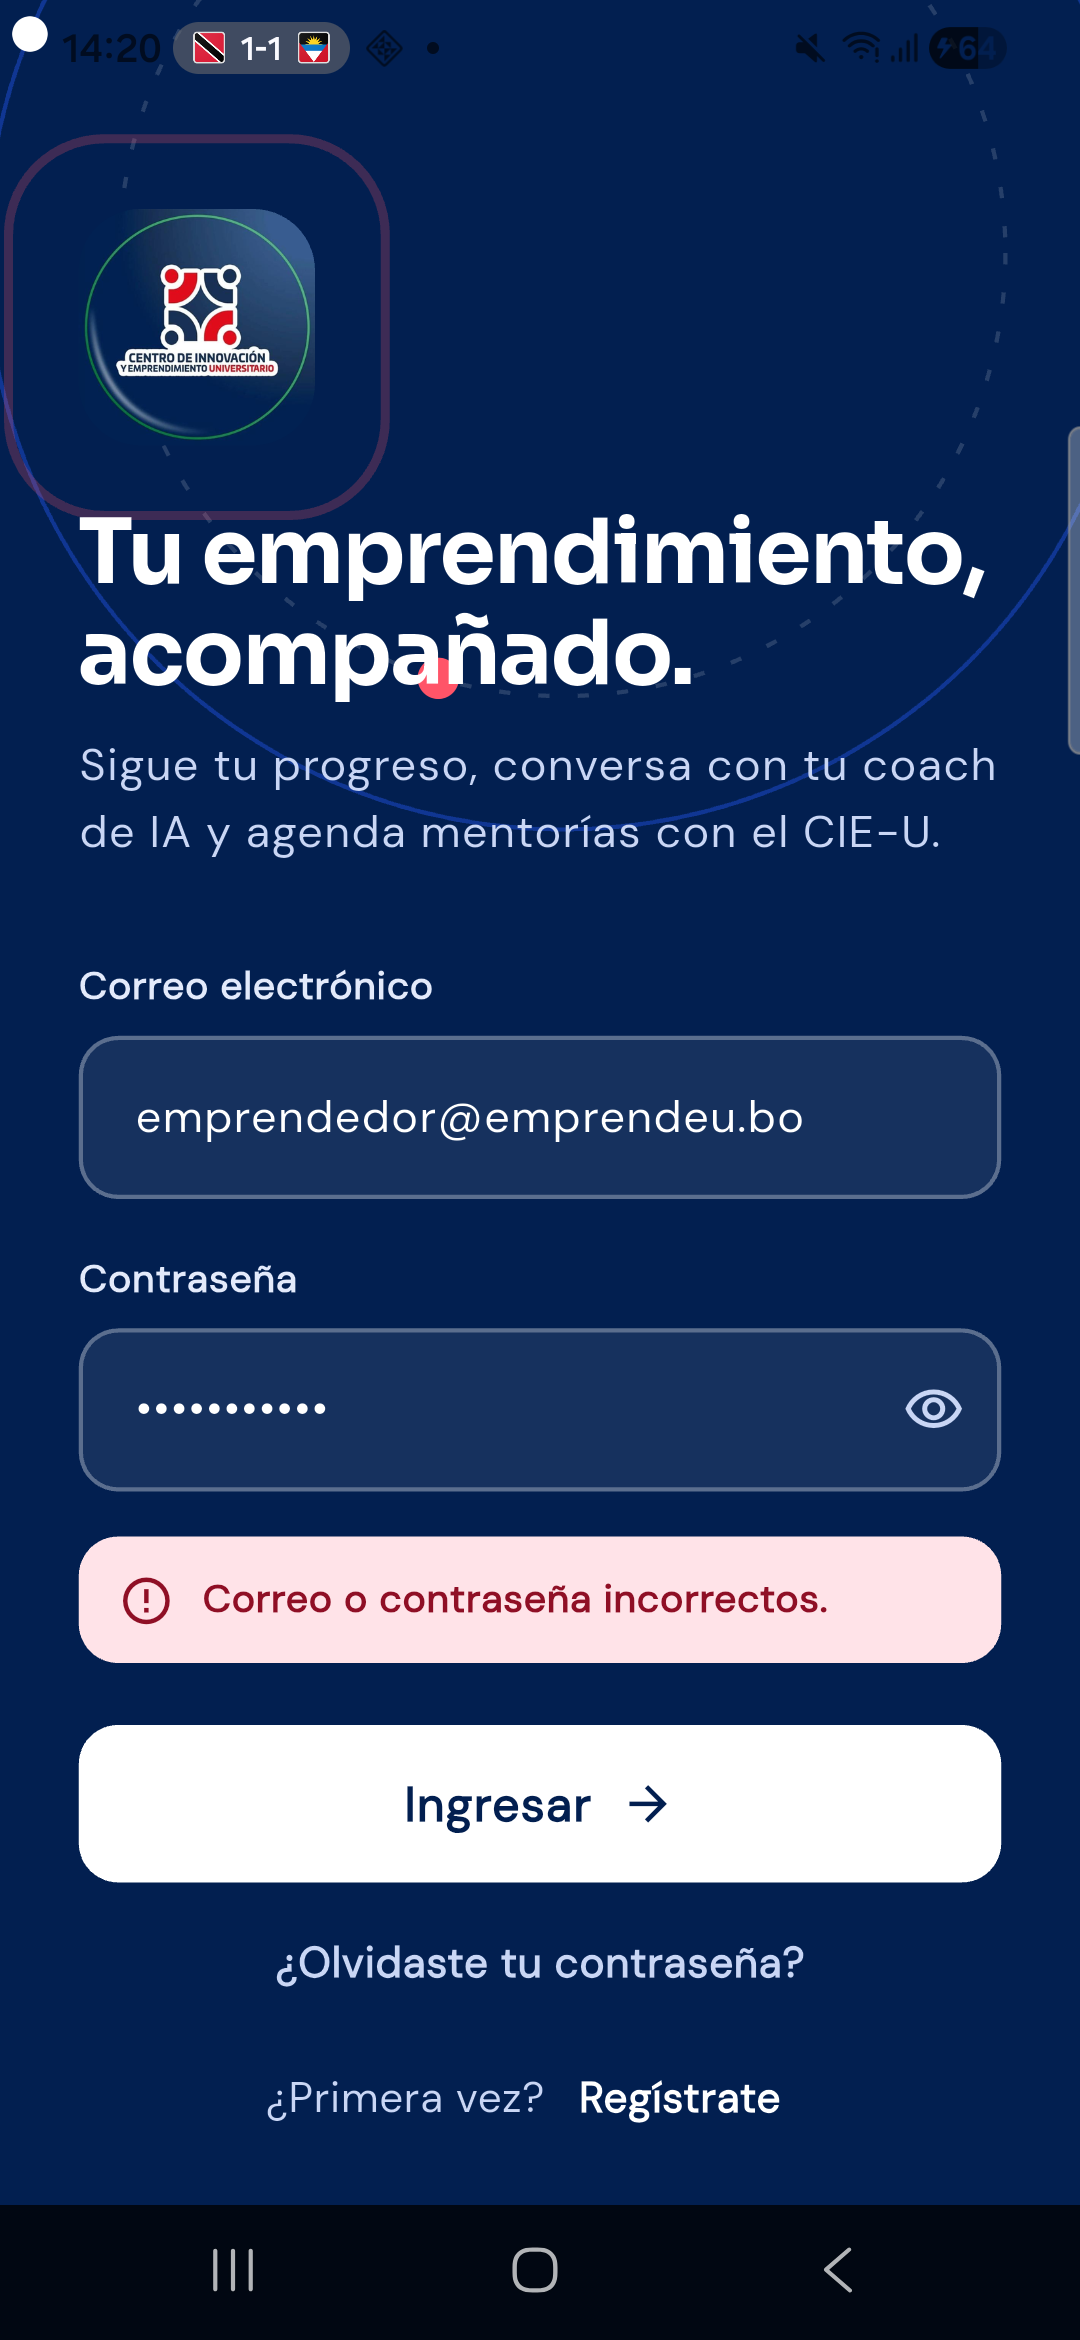
\includegraphics[height=0.52\textheight,keepaspectratio]{imagenes/movil_login_error.png}}
\par\vspace{3pt}\begin{flushleft}\small \textit{Nota.} Se muestra el aviso «Correo o contraseña incorrectos.» cuando las credenciales no son válidas.\end{flushleft}
\end{figure}

\textit{Validaciones:} «Ingresa tu correo electrónico.», «Ingresa un correo válido.» e «Ingresa tu contraseña.». Tras varios intentos fallidos el sistema limita los intentos y pide esperar unos segundos. Si la cuenta está deshabilitada aparece «Tu cuenta está deshabilitada. Contacta al CIE-U.».

\subsection*{3.3. Registro y postulación}

\addcontentsline{toc}{subsection}{3.3. Registro y postulación}

\textbf{Crear cuenta.} Desde «Solicitar acceso» en el inicio de sesión web, o «Regístrate» en la aplicación móvil, se completa «Nombre completo», «Correo electrónico», contraseña (mínimo 8 caracteres) y «Confirmar contraseña», y se selecciona «Crear cuenta». La cuenta creada es siempre de emprendedor; en el panel web no ingresa hasta que un administrador le asigne un rol de personal.

\begin{figure}[H]\singlespacing
\caption{Formulario de registro web}\label{fig:web_register}
\centering\fbox{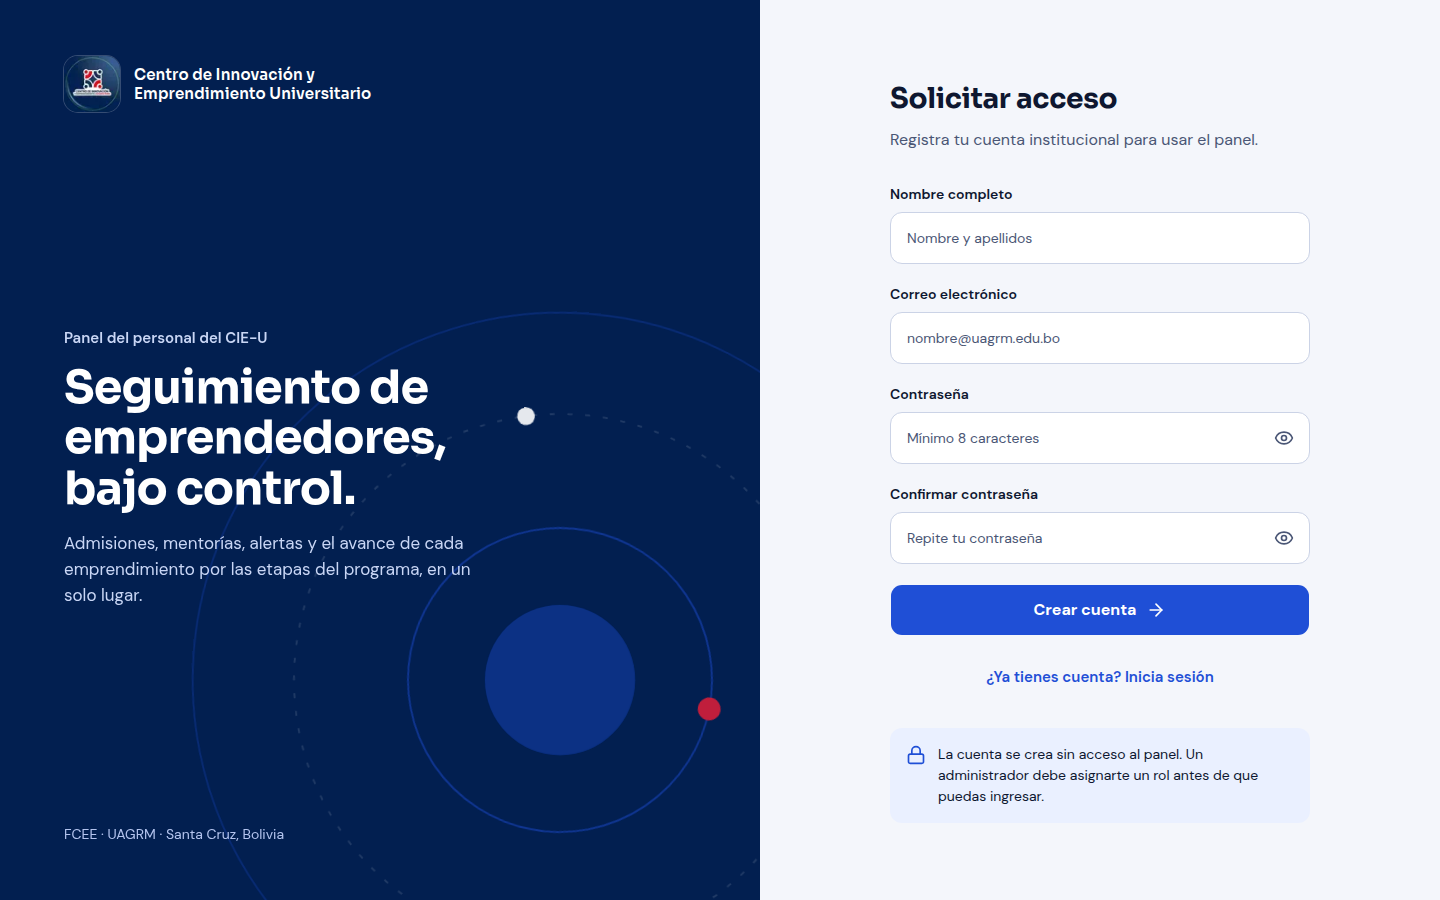
\includegraphics[width=0.97\textwidth,keepaspectratio]{imagenes/web_register.png}}
\par\vspace{3pt}\begin{flushleft}\small \textit{Nota.} El registro crea una cuenta de emprendedor.\end{flushleft}
\end{figure}

\textbf{Postular un emprendimiento.} La página pública «Postula tu emprendimiento» (Figura~\ref{fig:web_apply}) no requiere cuenta.

\begin{enumerate}
\item Seleccionar «Postular» en la página de inicio.
\item Completar «Nombre», «Apellidos», «Correo electrónico», «Documento de identidad» y «Nombre de tu emprendimiento». Los campos «Sector», «Teléfono» y «Cuéntanos de tu idea» son opcionales.
\item Enviar el formulario.
\item El sistema confirma: «Recibimos tu postulación. El equipo del CIE-U la evaluará y se pondrá en contacto contigo.».
\end{enumerate}

\begin{figure}[H]\singlespacing
\caption{Formulario de postulación}\label{fig:web_apply}
\centering\fbox{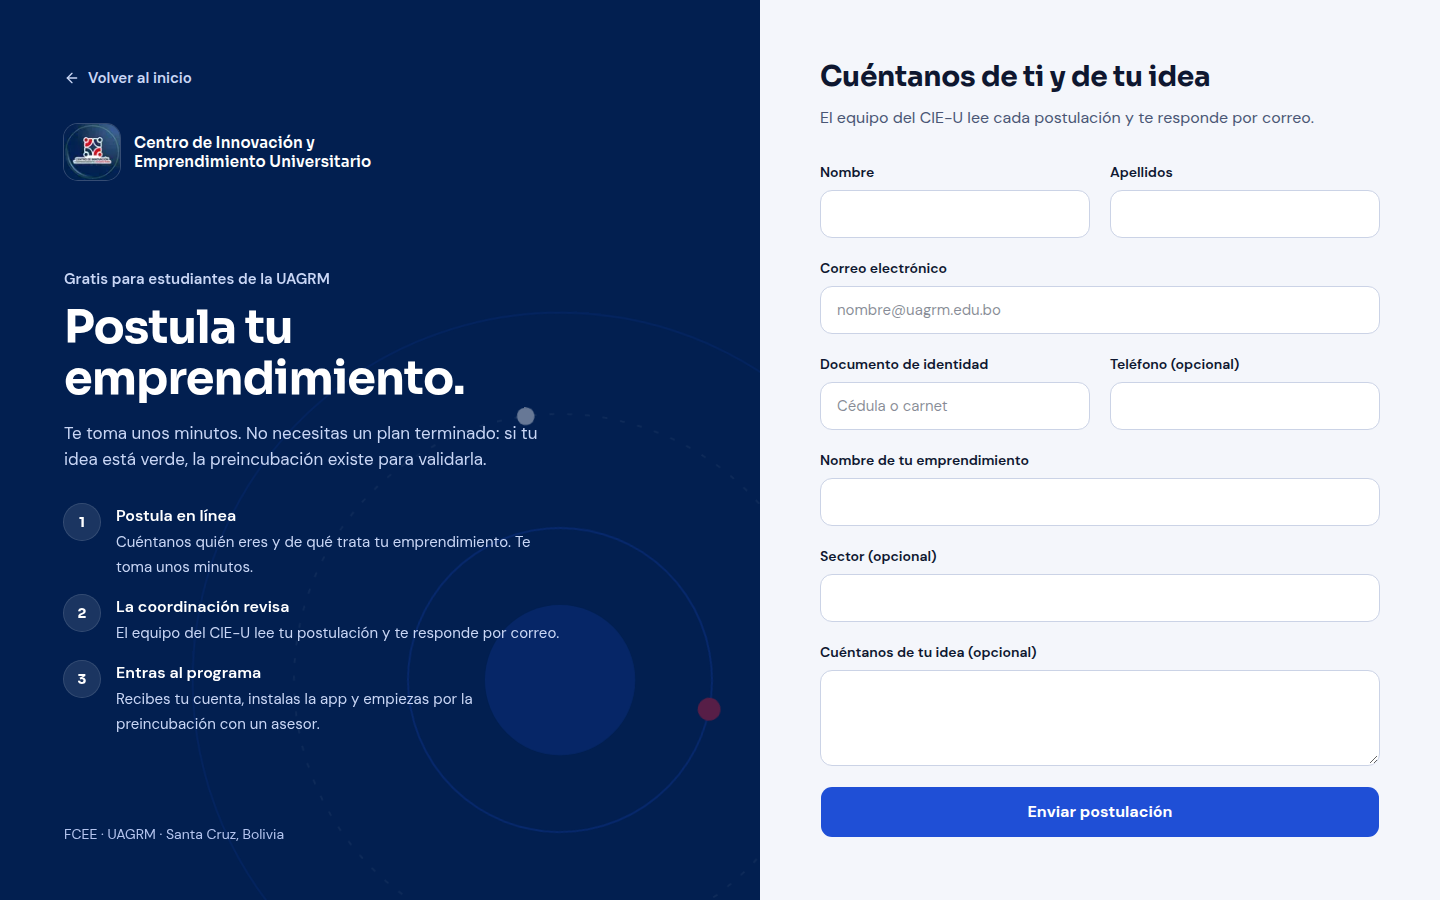
\includegraphics[width=0.97\textwidth,keepaspectratio]{imagenes/web_apply.png}}
\par\vspace{3pt}\begin{flushleft}\small \textit{Nota.} Gratis para estudiantes de la UAGRM.\end{flushleft}
\end{figure}

Si ya existe una postulación pendiente con el mismo correo aparece «Ya tenemos una postulación pendiente con ese correo.».

\subsection*{3.4. Recuperación de contraseña}

\addcontentsline{toc}{subsection}{3.4. Recuperación de contraseña}

\begin{enumerate}
\item Seleccionar «¿Olvidaste tu contraseña?» en la pantalla de ingreso.
\item Escribir el correo y seleccionar «Enviar código». El sistema envía un código de 6 dígitos que vence en 15 minutos. La respuesta es la misma exista o no la cuenta.
\item Escribir el «Código de 6 dígitos», la «Nueva contraseña» y su confirmación.
\item Seleccionar «Restablecer contraseña» (en la aplicación móvil, «Restablecer»).
\item El sistema redirige al ingreso con el aviso «Contraseña actualizada. Ya puedes iniciar sesión.».
\end{enumerate}

\begin{figure}[H]\singlespacing
\caption{Solicitud del código de recuperación}\label{fig:web_forgot}
\centering\fbox{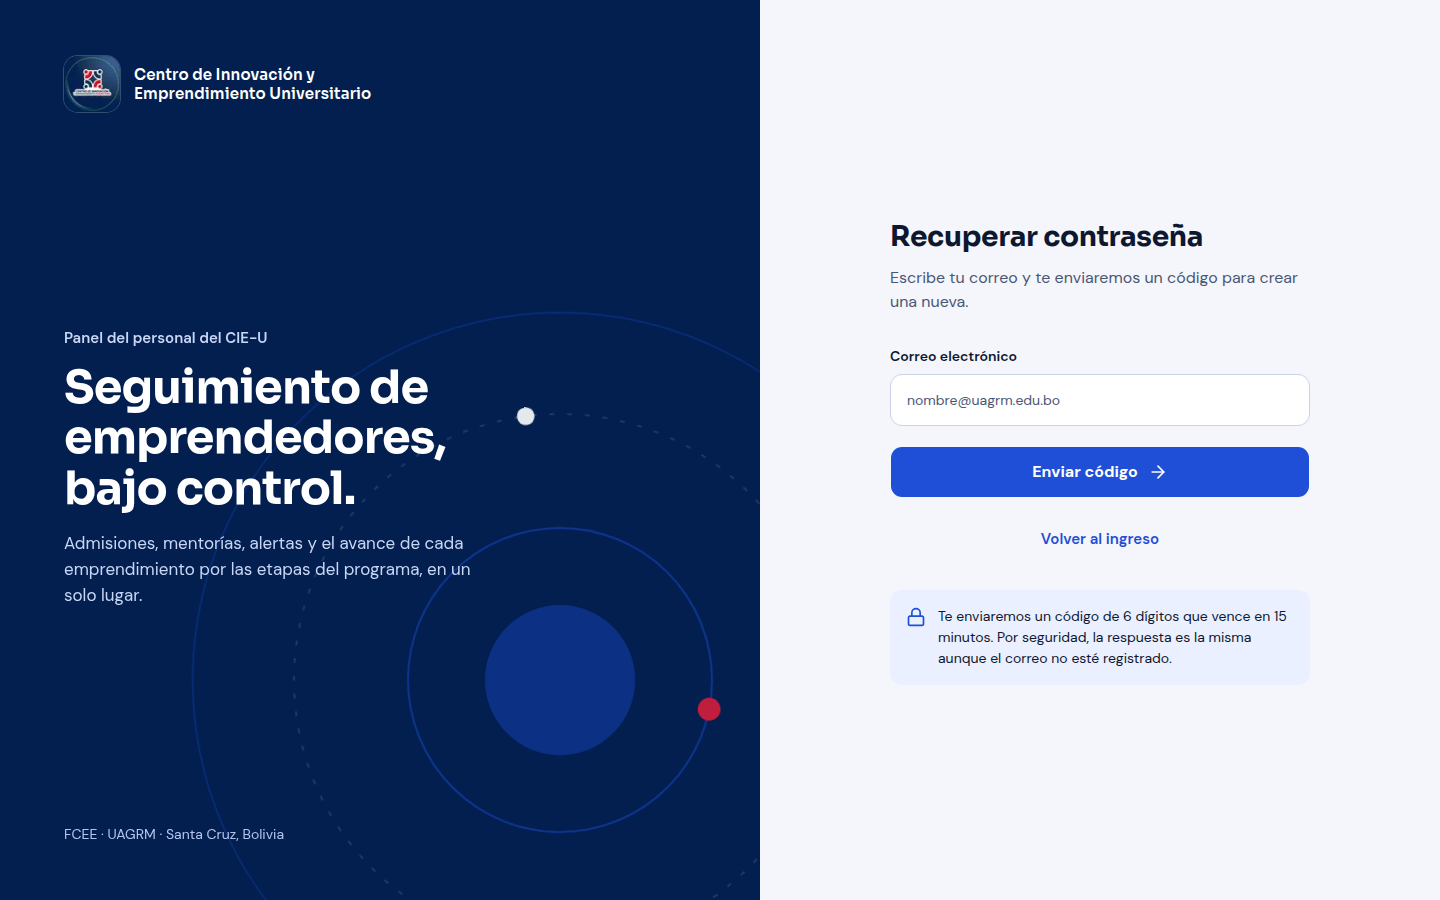
\includegraphics[width=0.97\textwidth,keepaspectratio]{imagenes/web_forgot.png}}
\par\vspace{3pt}\begin{flushleft}\small \textit{Nota.} Pantalla «Recupera tu contraseña».\end{flushleft}
\end{figure}

Si el código es incorrecto o venció: «El código no es válido o ya venció. Pide uno nuevo.». Si el servicio de correo no está disponible: «No pudimos enviar el correo. Intenta de nuevo en unos minutos.».

\subsection*{3.5. Descripción de la pantalla inicial}

\addcontentsline{toc}{subsection}{3.5. Descripción de la pantalla inicial}

Tras ingresar, el personal ve «Resumen» (Figura~\ref{fig:web_admin_panel}). La aplicación móvil abre «Inicio» (Figura~\ref{fig:movil_inicio}).

\subsection*{3.6. Navegación entre las secciones}

\addcontentsline{toc}{subsection}{3.6. Navegación entre las secciones}

En el panel web, el menú lateral agrupa las pantallas en Inicio, Programa, Acompañamiento y Configuración. En pantallas pequeñas el menú se abre como una hoja lateral. En la aplicación móvil, la barra inferior tiene cinco pestañas: Inicio, Camino, Mentorías, Coach y Perfil.

\subsection*{3.7. Cierre de sesión}

\addcontentsline{toc}{subsection}{3.7. Cierre de sesión}

En el panel web, seleccionar «Cerrar sesión» al pie del menú lateral. En la aplicación móvil, abrir la pestaña «Perfil» y tocar «Cerrar sesión»; esta acción borra los datos locales de la sesión.

\clearpage

\section*{CAPÍTULO 4. INTERFAZ GENERAL}

\addcontentsline{toc}{section}{CAPÍTULO 4. INTERFAZ GENERAL}

\subsection*{4.1. Descripción de la interfaz}

\addcontentsline{toc}{subsection}{4.1. Descripción de la interfaz}

Ambas aplicaciones usan la identidad visual del CIE-U: fondo claro, azul marino para el menú y azul para los botones principales.

\subsection*{4.2. Menú principal}

\addcontentsline{toc}{subsection}{4.2. Menú principal}

El menú lateral del panel web muestra solo las secciones permitidas. Al pie aparece la tarjeta de la persona con su rol y el acceso a «Mi cuenta». «Alertas» muestra una insignia con el número de alertas abiertas.

\begin{table}[H]\singlespacing\small
\caption{Menú del panel web}
\begin{tabularx}{\textwidth}{XX}
\toprule
\textbf{Grupo} & \textbf{Opciones} \\
\midrule
\relax Inicio & Resumen, Indicadores, Reportes \\
\relax Programa & Admisiones, Emprendedores, Emprendimientos, Necesidades, Alertas, Salud \\
\relax Acompañamiento & Asignaciones, Mi disponibilidad, Sesiones, Capacitaciones \\
\relax Configuración & Usuarios, Roles y permisos, Parámetros, Catálogos y XP, Base de conocimiento, Auditoría \\
\bottomrule
\end{tabularx}
\end{table}

\subsection*{4.3. Barra de navegación}

\addcontentsline{toc}{subsection}{4.3. Barra de navegación}

La aplicación móvil dispone de una barra inferior con cinco pestañas. Tocar de nuevo la pestaña activa devuelve a su pantalla inicial. Las pantallas secundarias tienen una flecha de regreso en la esquina superior izquierda.

\subsection*{4.4. Botones y controles}

\addcontentsline{toc}{subsection}{4.4. Botones y controles}

Los botones azules ejecutan la acción principal («Nuevo usuario», «Guardar cambios»). Los filtros aparecen como botones tipo píldora («Todos», «Activo», «Pausado»). Los interruptores habilitan o deshabilitan una opción. Las acciones de creación y edición se abren en hojas laterales.

\subsection*{4.5. Formularios}

\addcontentsline{toc}{subsection}{4.5. Formularios}

Los campos obligatorios se validan antes de enviar y el mensaje aparece bajo el campo. Cuando el sistema crea una cuenta de emprendedor o de personal muestra una «Contraseña temporal» una sola vez, con un botón para copiarla.

\subsection*{4.6. Mensajes y notificaciones}

\addcontentsline{toc}{subsection}{4.6. Mensajes y notificaciones}

Las confirmaciones aparecen como avisos breves, por ejemplo «Emprendimiento creado: \ldots{}», casi siempre seguidos de «Registrado en auditoría.». En la aplicación móvil, la campana de «Inicio» abre la bandeja de «Notificaciones», con los avisos de mentorías, compromisos, capacitaciones y logros.

\subsection*{4.7. Elementos visuales relevantes}

\addcontentsline{toc}{subsection}{4.7. Elementos visuales relevantes}

\begin{itemize}
\item \textbf{Semáforo de salud:} verde (Bien), ámbar (Vigilar) y rojo (Atender ya), siempre acompañado de texto.
\item \textbf{Trayecto de etapas:} muestra la etapa actual del emprendimiento.
\item \textbf{Botón de ayuda:} círculo azul en la esquina inferior derecha del panel web, que abre el asistente de ayuda.
\end{itemize}

\clearpage

\section*{CAPÍTULO 5. FUNCIONALIDADES DEL SISTEMA}

\addcontentsline{toc}{section}{CAPÍTULO 5. FUNCIONALIDADES DEL SISTEMA}

\subsection*{5.1. Panel web: Inicio}

\addcontentsline{toc}{subsection}{5.1. Panel web: Inicio}

\subsubsection*{5.1.1. Resumen}

\addcontentsline{toc}{subsubsection}{5.1.1. Resumen}

\textbf{Descripción.} Muestra el estado del programa: emprendimientos activos, alertas abiertas, usuarios por rol, estado de los servicios y actividad reciente. \textbf{Roles:} quienes tienen consulta de Indicadores y reportes (administrador y coordinador). \textbf{Acceso:} menú Inicio $\rightarrow$ «Resumen».

\begin{figure}[H]\singlespacing
\caption{Pantalla Resumen del administrador}\label{fig:web_admin_panel}
\centering\fbox{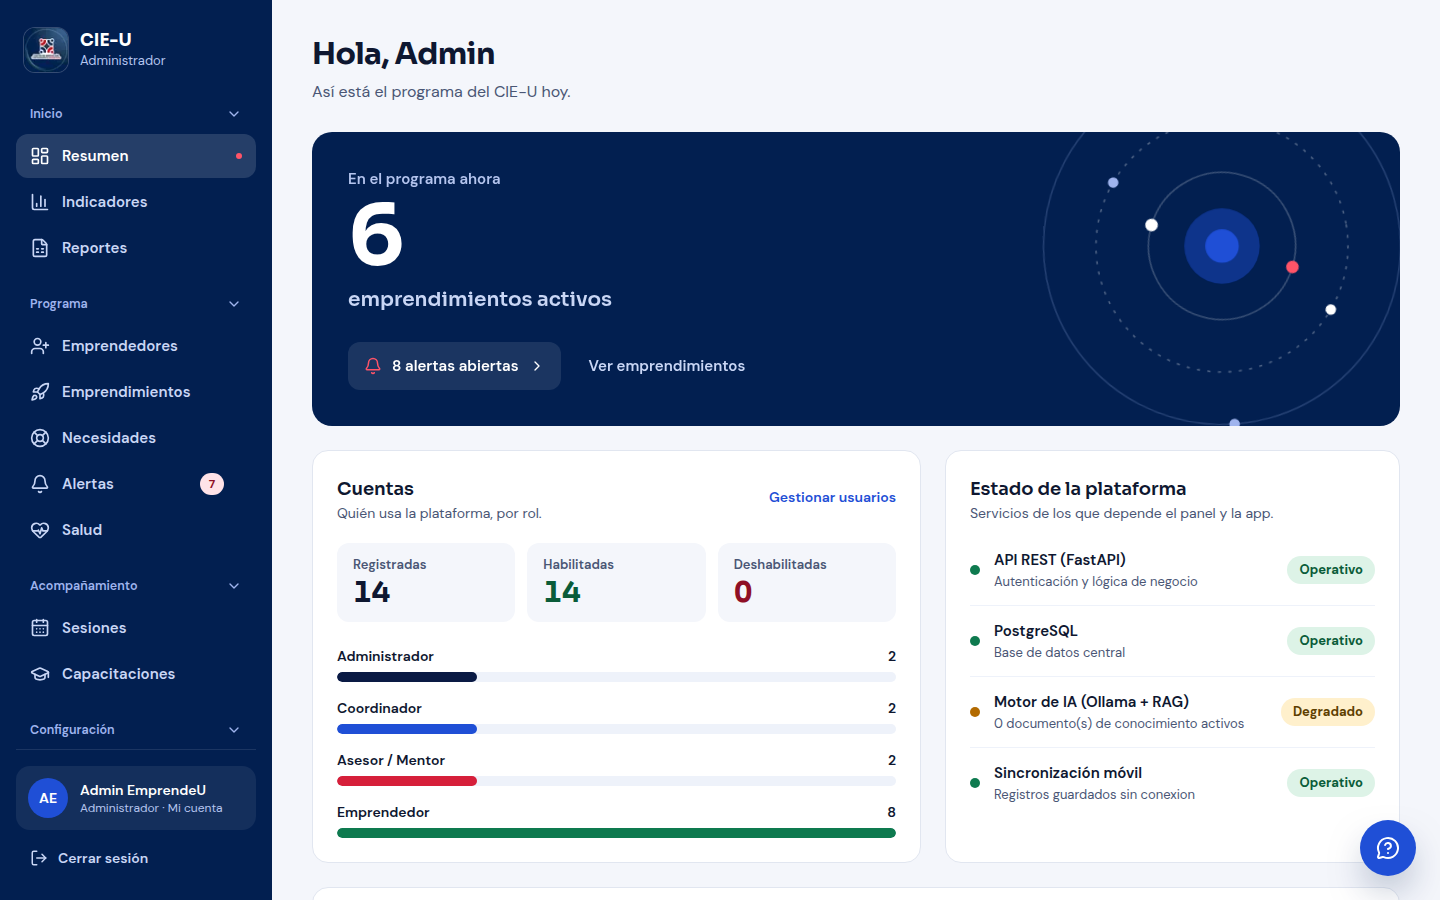
\includegraphics[width=0.97\textwidth,keepaspectratio]{imagenes/web_admin_panel.png}}
\par\vspace{3pt}\begin{flushleft}\small \textit{Nota.} Incluye accesos rápidos a alertas y emprendimientos.\end{flushleft}
\end{figure}

\textbf{Restricciones.} Un asesor no tiene este permiso en la configuración inicial y ve «Sin acceso a el resumen» (Figura~\ref{fig:web_asesor_panel}). Para trabajar puede usar otra opción del menú.

\begin{figure}[H]\singlespacing
\caption{Pantalla Resumen vista por un asesor}\label{fig:web_asesor_panel}
\centering\fbox{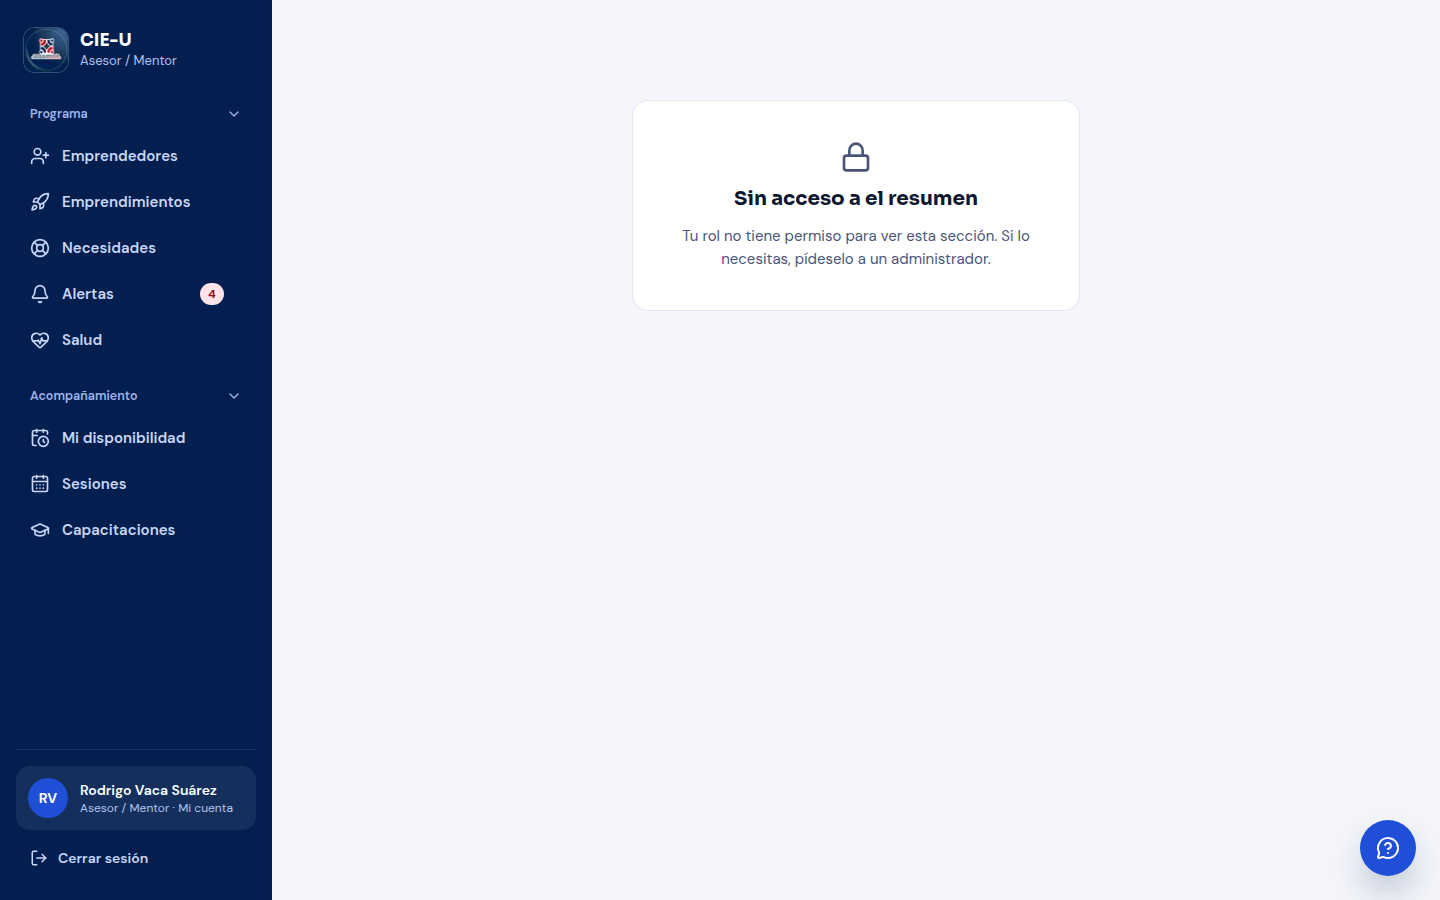
\includegraphics[width=0.97\textwidth,keepaspectratio]{imagenes/web_asesor_panel.png}}
\par\vspace{3pt}\begin{flushleft}\small \textit{Nota.} Ejemplo de mensaje de acceso restringido junto al tutorial inicial.\end{flushleft}
\end{figure}

\subsubsection*{5.1.2. Indicadores}

\addcontentsline{toc}{subsubsection}{5.1.2. Indicadores}

\textbf{Descripción.} Presenta cifras del programa: emprendimientos por etapa, sesiones realizadas, avances, compromisos vencidos y alertas por tipo. \textbf{Acceso:} «Indicadores».

\begin{enumerate}
\item Abrir «Indicadores».
\item Elegir las fechas «Desde» y «Hasta» y la etapa («Todas las etapas»).
\item Seleccionar «Aplicar».
\end{enumerate}

\begin{figure}[H]\singlespacing
\caption{Indicadores del programa}\label{fig:web_admin_dashboard}
\centering\fbox{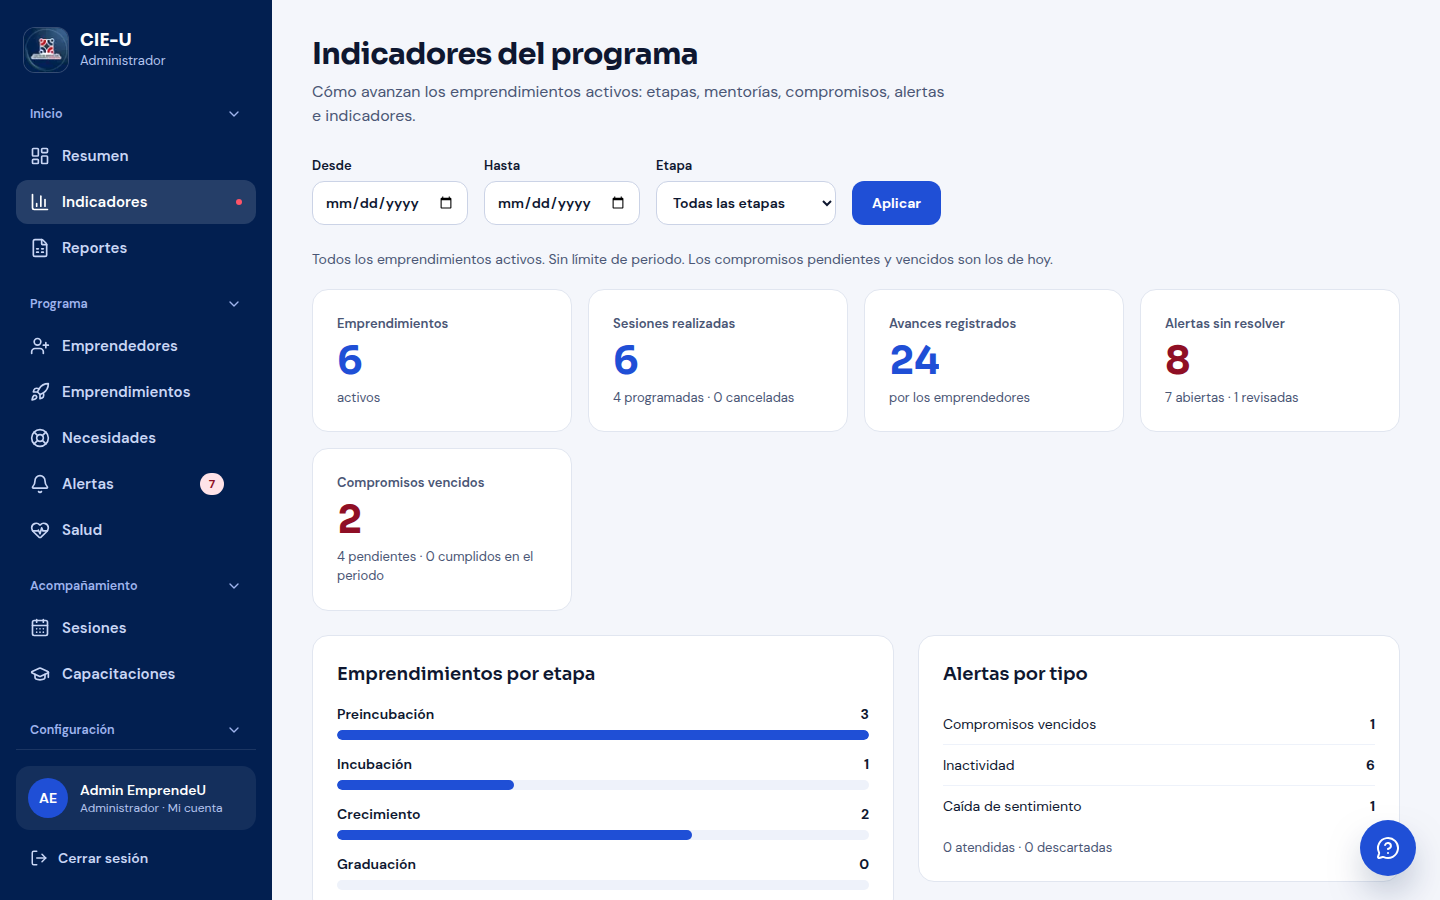
\includegraphics[width=0.97\textwidth,keepaspectratio]{imagenes/web_admin_dashboard.png}}
\par\vspace{3pt}\begin{flushleft}\small \textit{Nota.} Los filtros se aplican a todas las tarjetas y tablas.\end{flushleft}
\end{figure}

\subsubsection*{5.1.3. Reportes}

\addcontentsline{toc}{subsubsection}{5.1.3. Reportes}

\textbf{Descripción.} Permite revisar y descargar cuatro reportes: «Resumen por emprendimiento», «Sesiones de mentoría», «Alertas» e «Indicadores».

\begin{enumerate}
\item Abrir «Reportes» y seleccionar la pestaña del reporte.
\item Elegir el periodo y la etapa, y seleccionar «Aplicar».
\item Revisar la vista previa (hasta 50 filas).
\item Seleccionar «Exportar Excel» o «Exportar CSV».
\end{enumerate}

\begin{figure}[H]\singlespacing
\caption{Reportes con vista previa}\label{fig:web_admin_reports}
\centering\fbox{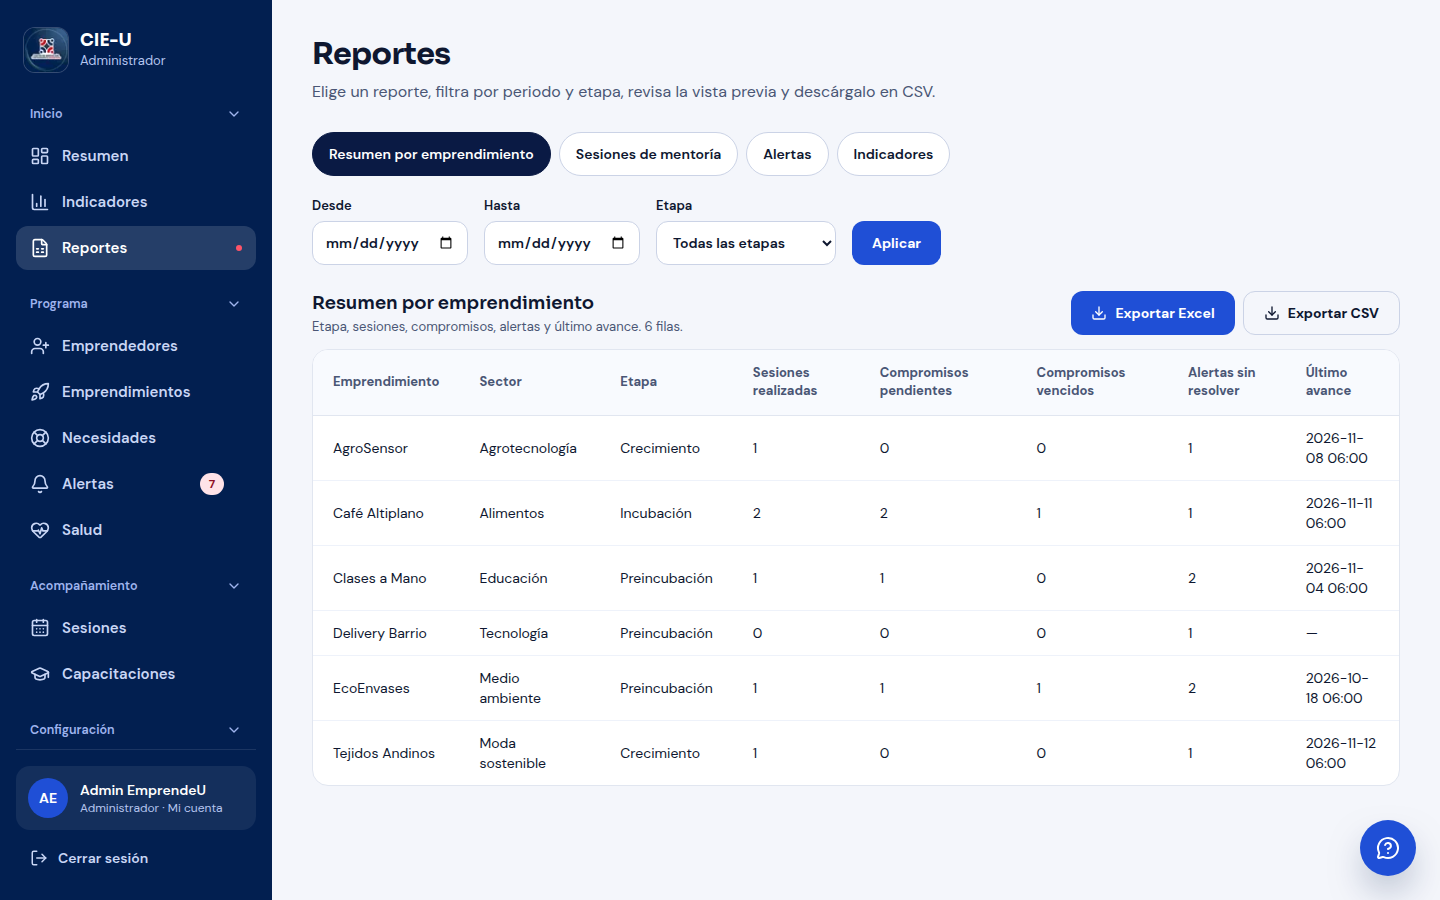
\includegraphics[width=0.97\textwidth,keepaspectratio]{imagenes/web_admin_reports.png}}
\par\vspace{3pt}\begin{flushleft}\small \textit{Nota.} Las descargas conservan los filtros aplicados.\end{flushleft}
\end{figure}

\subsection*{5.2. Panel web: Programa}

\addcontentsline{toc}{subsection}{5.2. Panel web: Programa}

\subsubsection*{5.2.1. Admisiones}

\addcontentsline{toc}{subsubsection}{5.2.1. Admisiones}

\textbf{Descripción.} Lista las postulaciones recibidas desde la web pública. \textbf{Roles:} coordinación (permiso de registro de emprendedores).

\begin{enumerate}
\item Abrir «Admisiones». Filtrar por estado (Pendientes, Admitidas, Rechazadas) o buscar por nombre, correo o emprendimiento.
\item Seleccionar «Revisar» en una postulación.
\item Elegir la decisión: admitir, rechazar o «Mantener pendiente». Si se rechaza, escribir el «Motivo del rechazo»; las «Observaciones» son opcionales.
\item Seleccionar «Confirmar decisión».
\item Al admitir, el sistema crea la cuenta y el emprendimiento y muestra la «Contraseña temporal».
\end{enumerate}

\begin{figure}[H]\singlespacing
\caption{Lista de admisiones}\label{fig:web_admin_admissions}
\centering\fbox{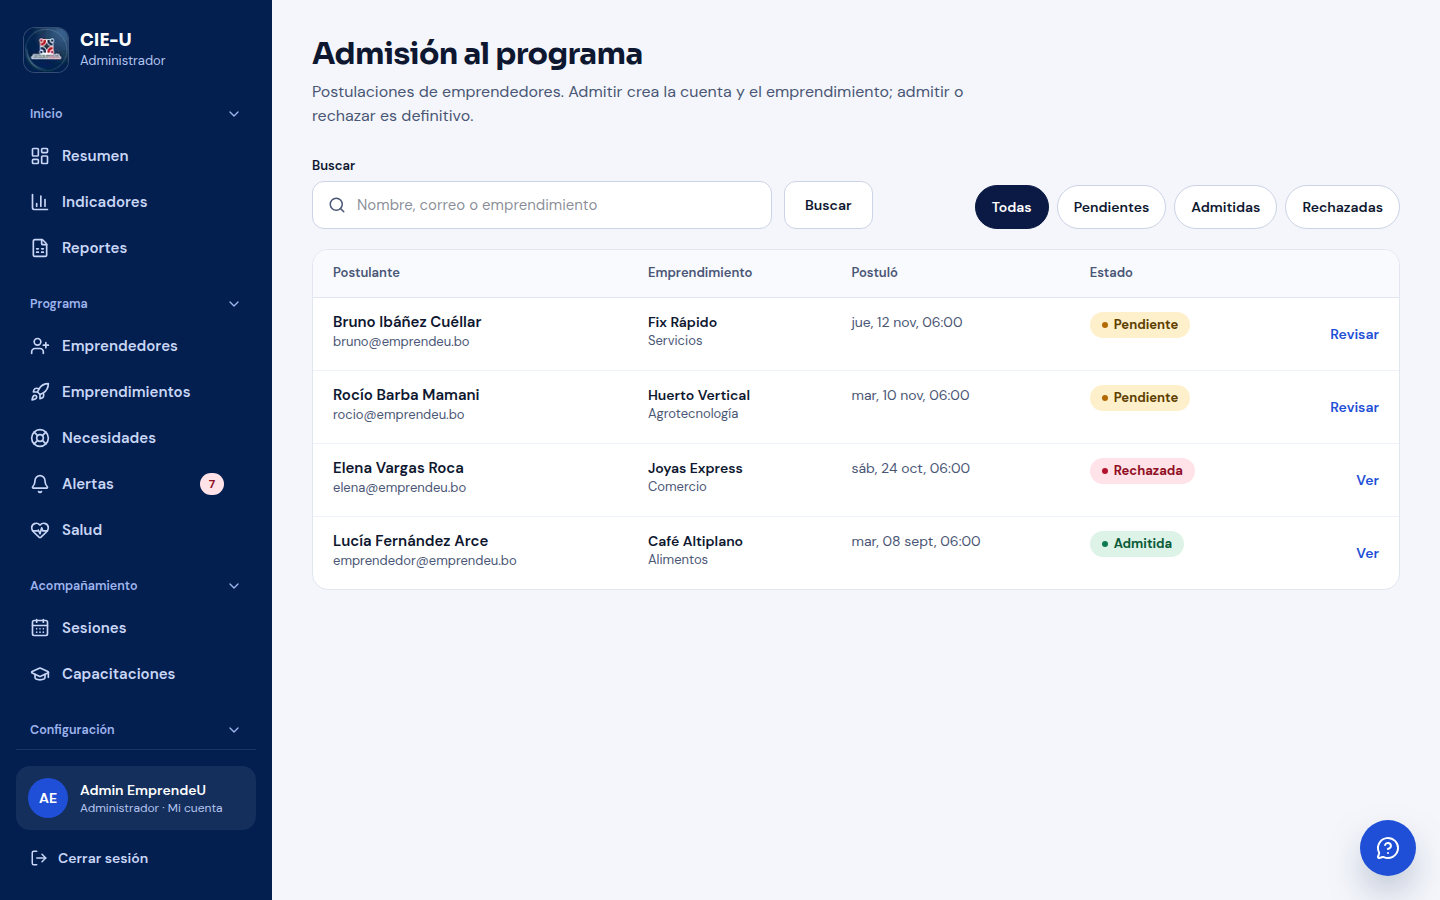
\includegraphics[width=0.97\textwidth,keepaspectratio]{imagenes/web_admin_admissions.png}}
\par\vspace{3pt}\begin{flushleft}\small \textit{Nota.} Los estados son pendiente, admitida y rechazada.\end{flushleft}
\end{figure}

\begin{figure}[H]\singlespacing
\caption{Detalle de una postulación}\label{fig:web_admission_detail}
\centering\fbox{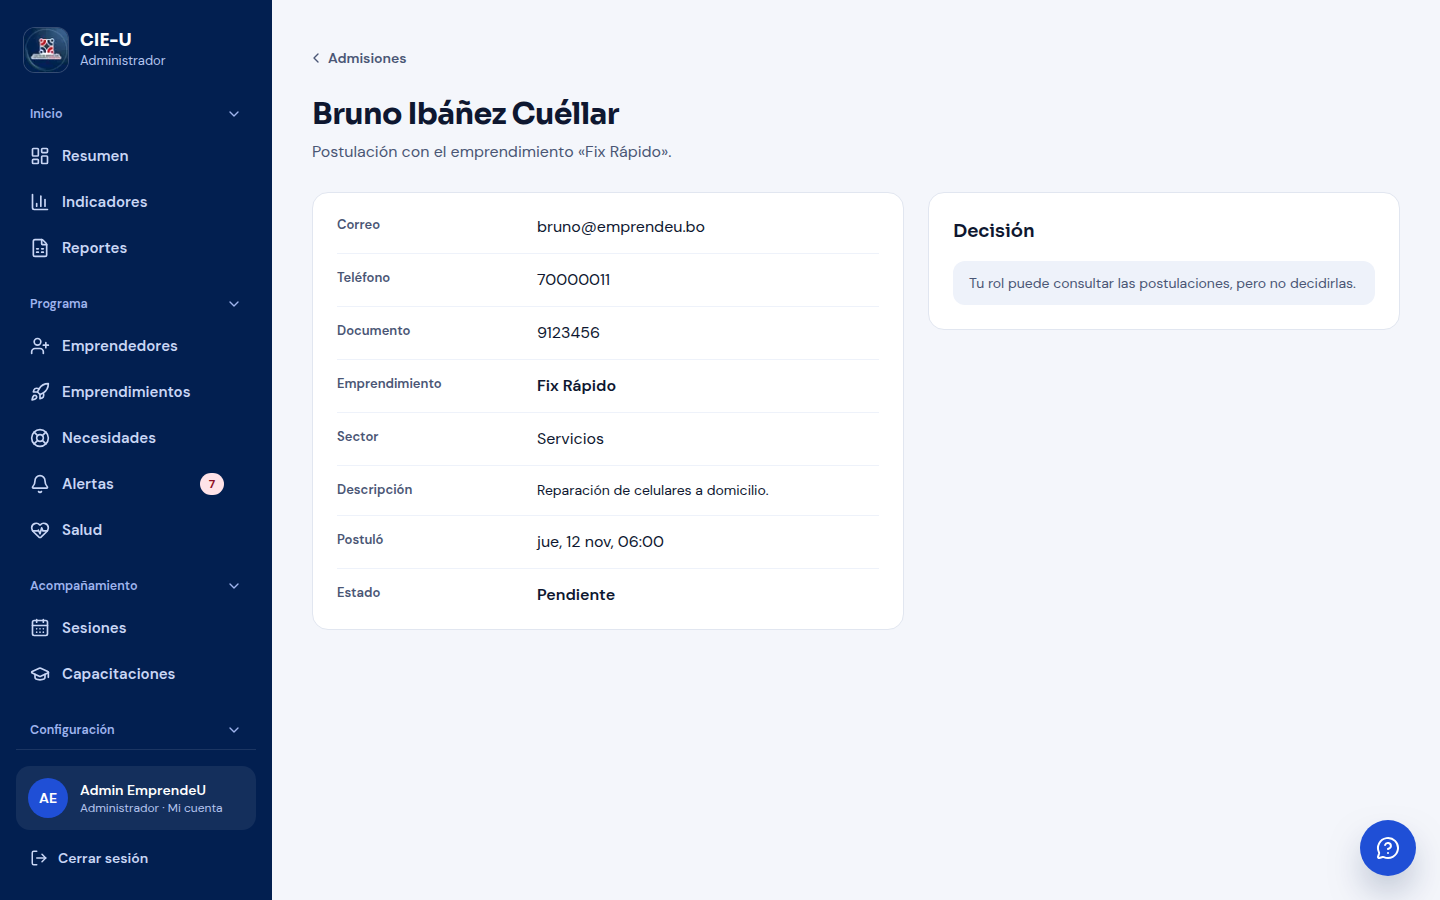
\includegraphics[width=0.97\textwidth,keepaspectratio]{imagenes/web_admission_detail.png}}
\par\vspace{3pt}\begin{flushleft}\small \textit{Nota.} Quien no puede decidir ve: «Tu rol puede consultar las postulaciones, pero no decidirlas.».\end{flushleft}
\end{figure}

\textbf{Restricciones.} Admitir o rechazar es definitivo. Errores frecuentes: «Falta el documento de identidad: no se puede admitir.», «Ese correo ya tiene una cuenta: no se puede crear otra.» y «Ese documento ya pertenece a otro emprendedor.».

\subsubsection*{5.2.2. Emprendedores}

\addcontentsline{toc}{subsubsection}{5.2.2. Emprendedores}

\textbf{Descripción.} Lista a las personas emprendedoras. El documento de identidad no puede repetirse.

\begin{enumerate}
\item Abrir «Emprendedores» y, si hace falta, buscar por nombre, correo o documento.
\item Seleccionar «Nuevo emprendedor».
\item Completar «Nombre completo», «Correo electrónico» y «Documento de identidad».
\item Seleccionar «Registrar emprendedor» y copiar la «Contraseña temporal» mostrada.
\end{enumerate}

\begin{figure}[H]\singlespacing
\caption{Lista de emprendedores}\label{fig:web_admin_entrepreneurs}
\centering\fbox{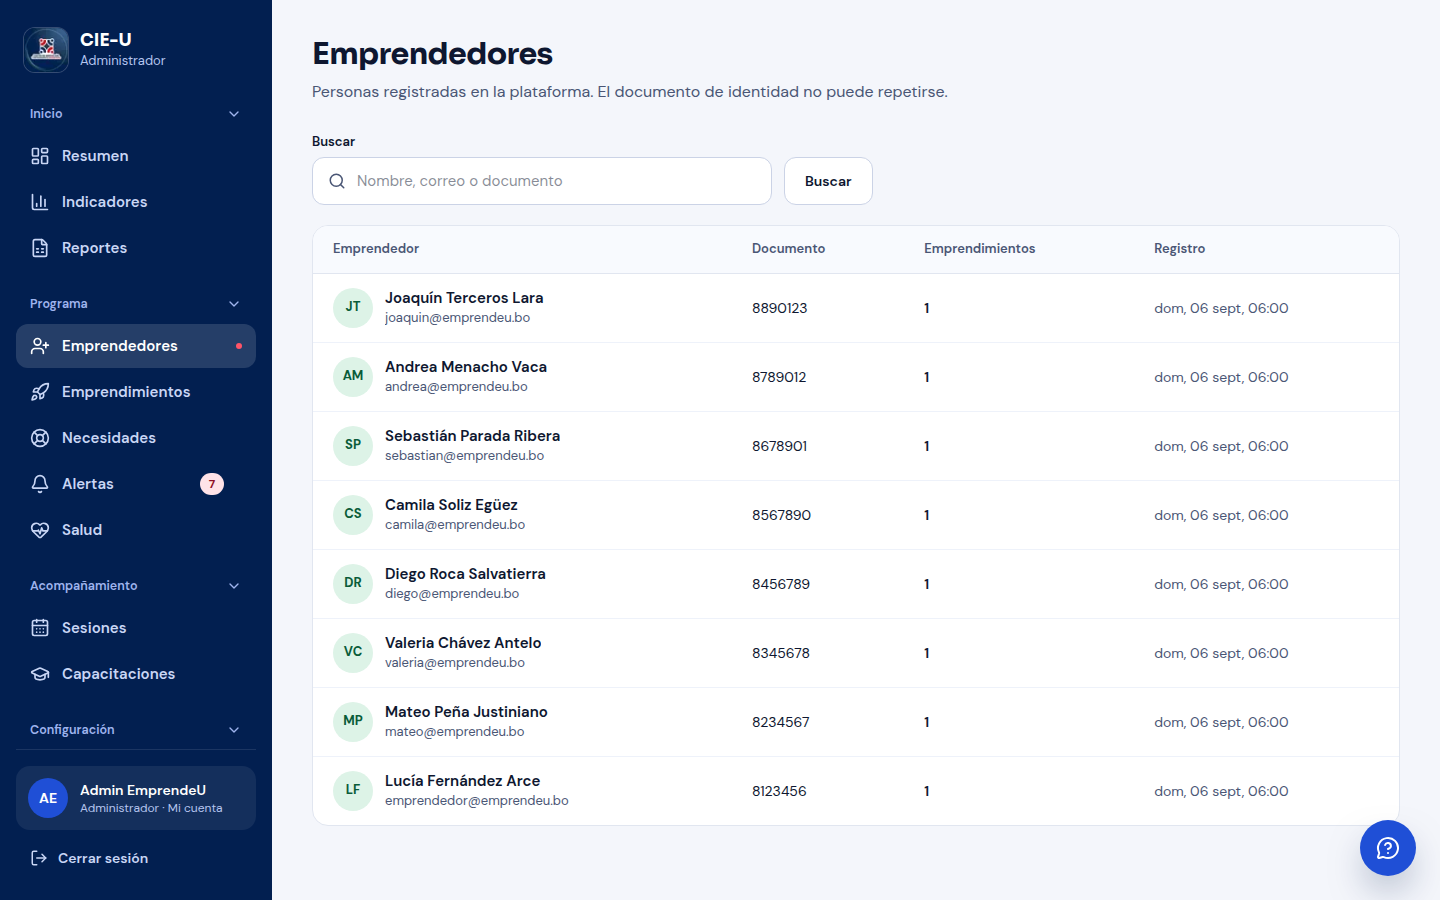
\includegraphics[width=0.97\textwidth,keepaspectratio]{imagenes/web_admin_entrepreneurs.png}}
\par\vspace{3pt}\begin{flushleft}\small \textit{Nota.} Muestra documento, cantidad de emprendimientos y fecha de registro.\end{flushleft}
\end{figure}

\textbf{Errores.} «Ese documento ya está registrado.», «Ese correo ya tiene cuenta.».

\subsubsection*{5.2.3. Emprendimientos}

\addcontentsline{toc}{subsubsection}{5.2.3. Emprendimientos}

\textbf{Descripción.} Gestiona los emprendimientos, su equipo y su etapa. \textbf{Roles:} consulta con permiso de emprendedores; crear (registro); editar (modificación); cambiar etapa (modificación de seguimiento).

\begin{enumerate}
\item Abrir «Emprendimientos». Filtrar por estado (Todos, Activo, Pausado, Cerrado) o buscar por nombre.
\item \textbf{Crear:} «Nuevo emprendimiento» $\rightarrow$ «Nombre del emprendimiento», «Sector», «Descripción», estado y equipo (cada integrante con su rol: Fundador, Cofundador o Miembro) $\rightarrow$ «Crear emprendimiento».
\item \textbf{Editar:} «Editar» $\rightarrow$ cambiar los datos $\rightarrow$ «Guardar cambios».
\item \textbf{Equipo:} abrir «Equipo» para agregar o quitar integrantes. El emprendimiento debe conservar al menos un integrante y tiene un máximo de 20.
\item \textbf{Cambiar etapa:} «Pasar a\ldots{}» (o «Avanzar etapa») $\rightarrow$ revisar los «Criterios de la etapa:» $\rightarrow$ agregar «Observaciones» (opcional) $\rightarrow$ confirmar.
\end{enumerate}

\begin{figure}[H]\singlespacing
\caption{Lista de emprendimientos}\label{fig:web_admin_ventures}
\centering\fbox{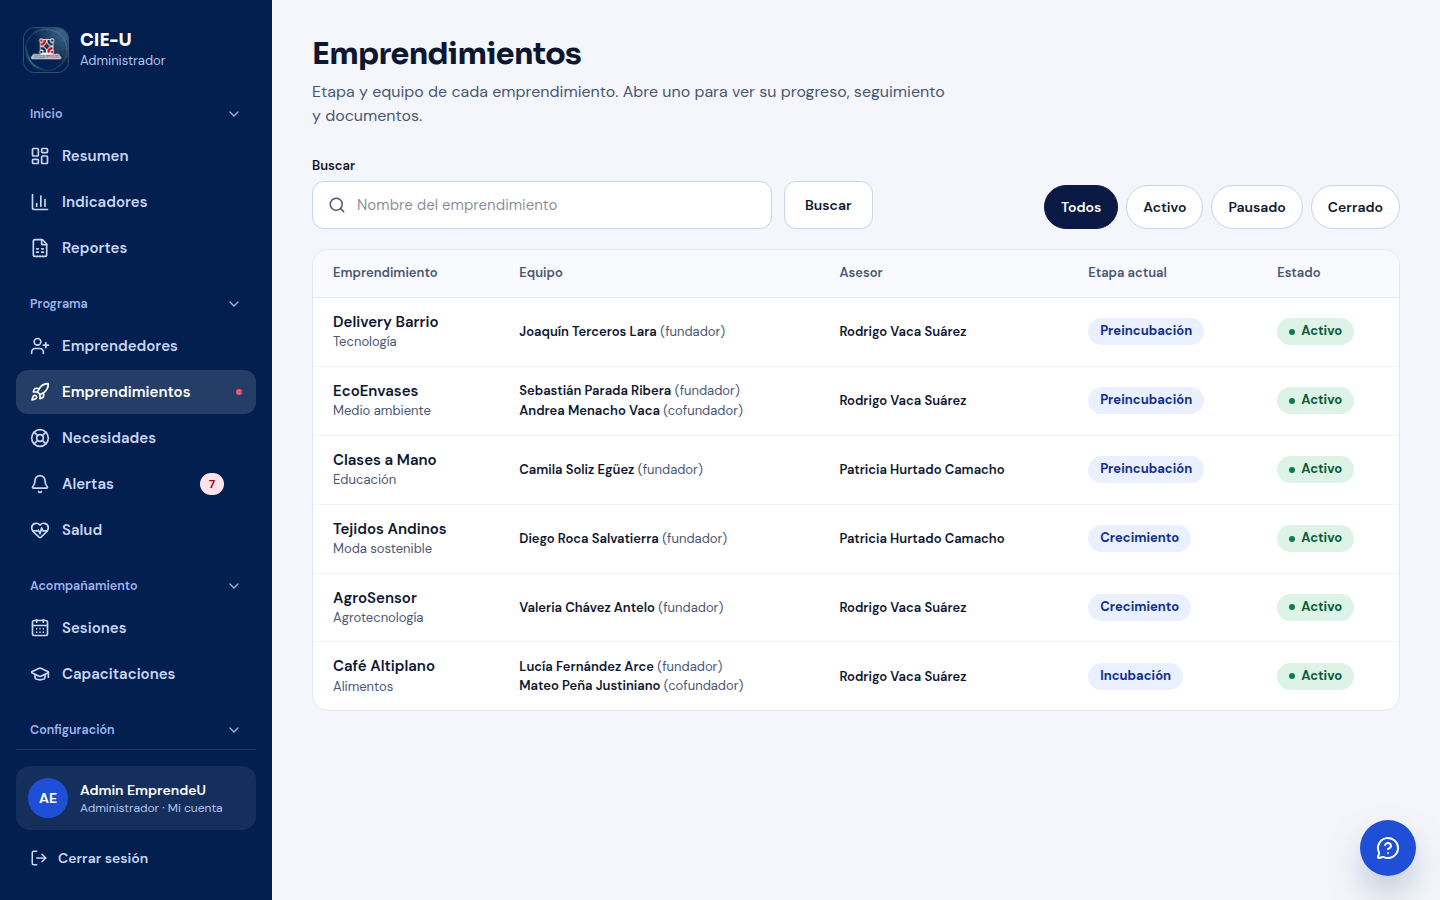
\includegraphics[width=0.97\textwidth,keepaspectratio]{imagenes/web_admin_ventures.png}}
\par\vspace{3pt}\begin{flushleft}\small \textit{Nota.} Cada fila muestra equipo, asesor, etapa y estado.\end{flushleft}
\end{figure}

\textbf{Restricciones.} La etapa solo avanza a la siguiente etapa activa. Mensajes: «Agrega al menos un emprendedor al equipo.», «Un emprendedor aparece dos veces en el equipo.», «Esa etapa está inactiva.».

\subsubsection*{5.2.4. Ficha del emprendimiento}

\addcontentsline{toc}{subsubsection}{5.2.4. Ficha del emprendimiento}

Al abrir un emprendimiento aparece su ficha con el trayecto de etapas y cinco pestañas.

\begin{itemize}
\item \textbf{Progreso:} XP acumulado, nivel, insignias, retos cumplidos e historial de XP. Es de solo lectura; los retos los cumple el emprendedor desde la aplicación.
\item \textbf{Seguimiento:} recomendaciones y compromisos. Con permiso de modificación de asesorías, «Marcar cumplido» cierra un compromiso.
\item \textbf{Etapas:} historial de cambios de etapa con fecha y observación.
\item \textbf{Documentos:} archivos del emprendimiento. «Subir documento» acepta PDF, imágenes, texto, hojas de cálculo, documentos y presentaciones; se pueden descargar y eliminar (con permiso).
\item \textbf{Historial:} eventos del emprendimiento, filtrables por tipo (sesión, avance, hito, recomendación, compromiso y etapa).
\end{itemize}

\begin{figure}[H]\singlespacing
\caption{Pestaña Progreso}\label{fig:web_venture_progress}
\centering\fbox{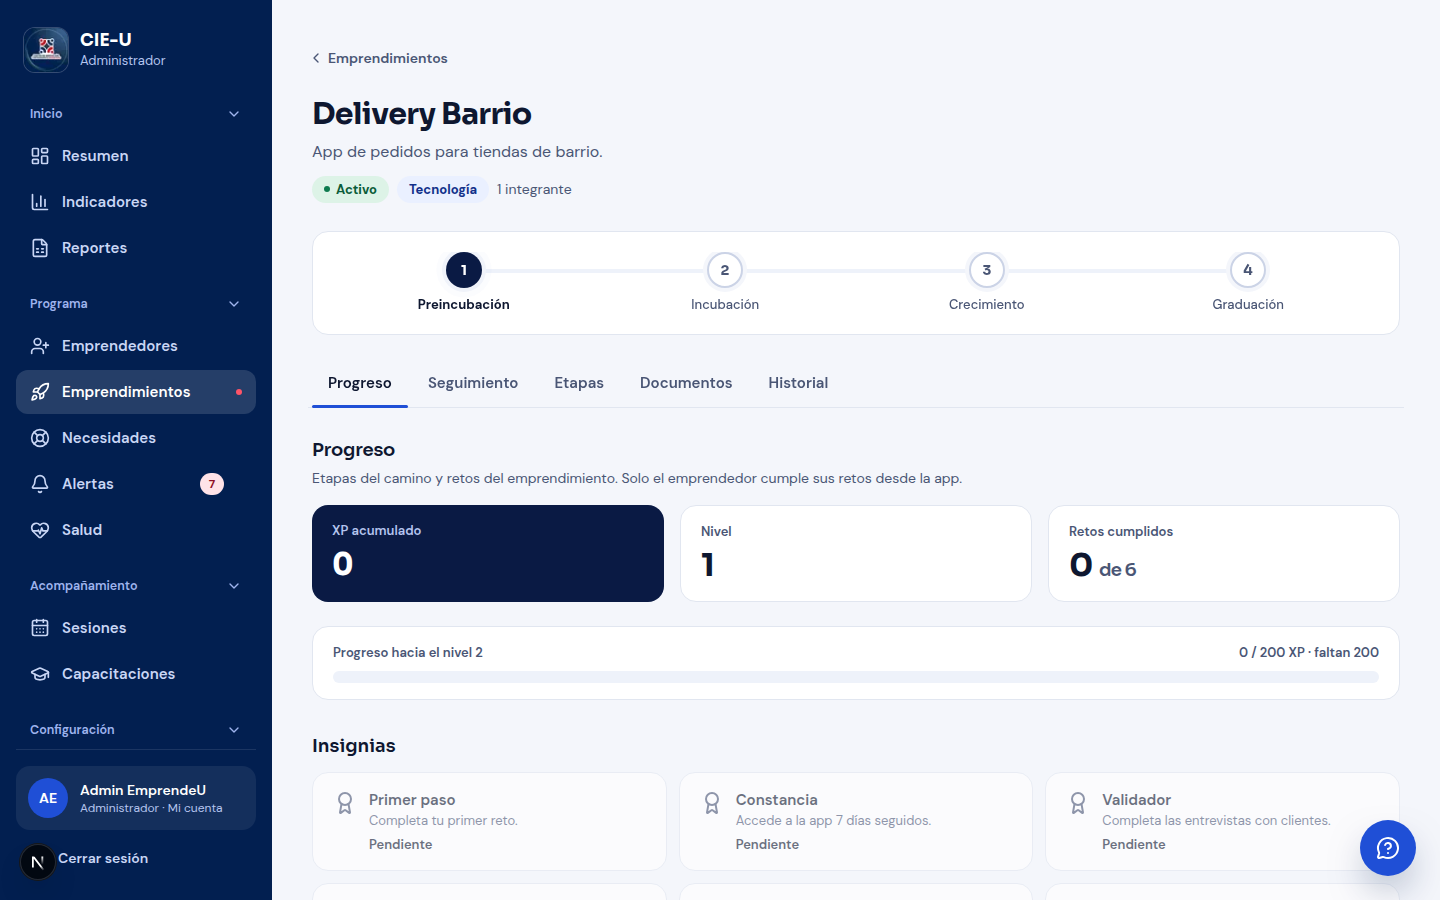
\includegraphics[width=0.97\textwidth,keepaspectratio]{imagenes/web_venture_progress.png}}
\par\vspace{3pt}\begin{flushleft}\small \textit{Nota.} El XP lo obtiene el emprendedor al cumplir retos en la aplicación móvil.\end{flushleft}
\end{figure}

\begin{figure}[H]\singlespacing
\caption{Pestaña Seguimiento}\label{fig:web_venture_follow-up}
\centering\fbox{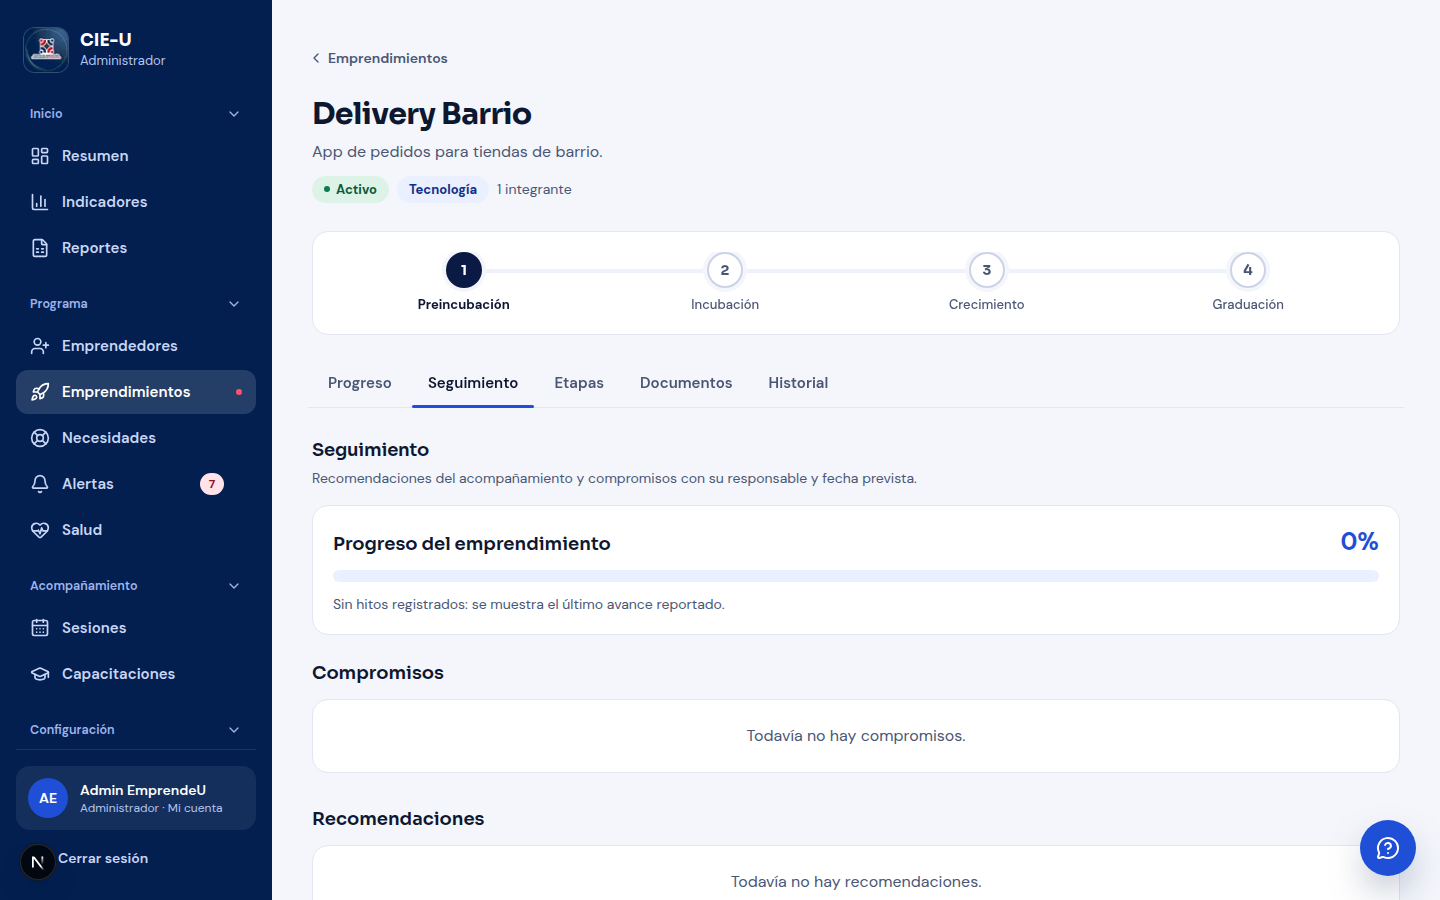
\includegraphics[width=0.97\textwidth,keepaspectratio]{imagenes/web_venture_follow-up.png}}
\par\vspace{3pt}\begin{flushleft}\small \textit{Nota.} Compromisos y recomendaciones del emprendimiento.\end{flushleft}
\end{figure}

\begin{figure}[H]\singlespacing
\caption{Pestaña Etapas}\label{fig:web_venture_stages}
\centering\fbox{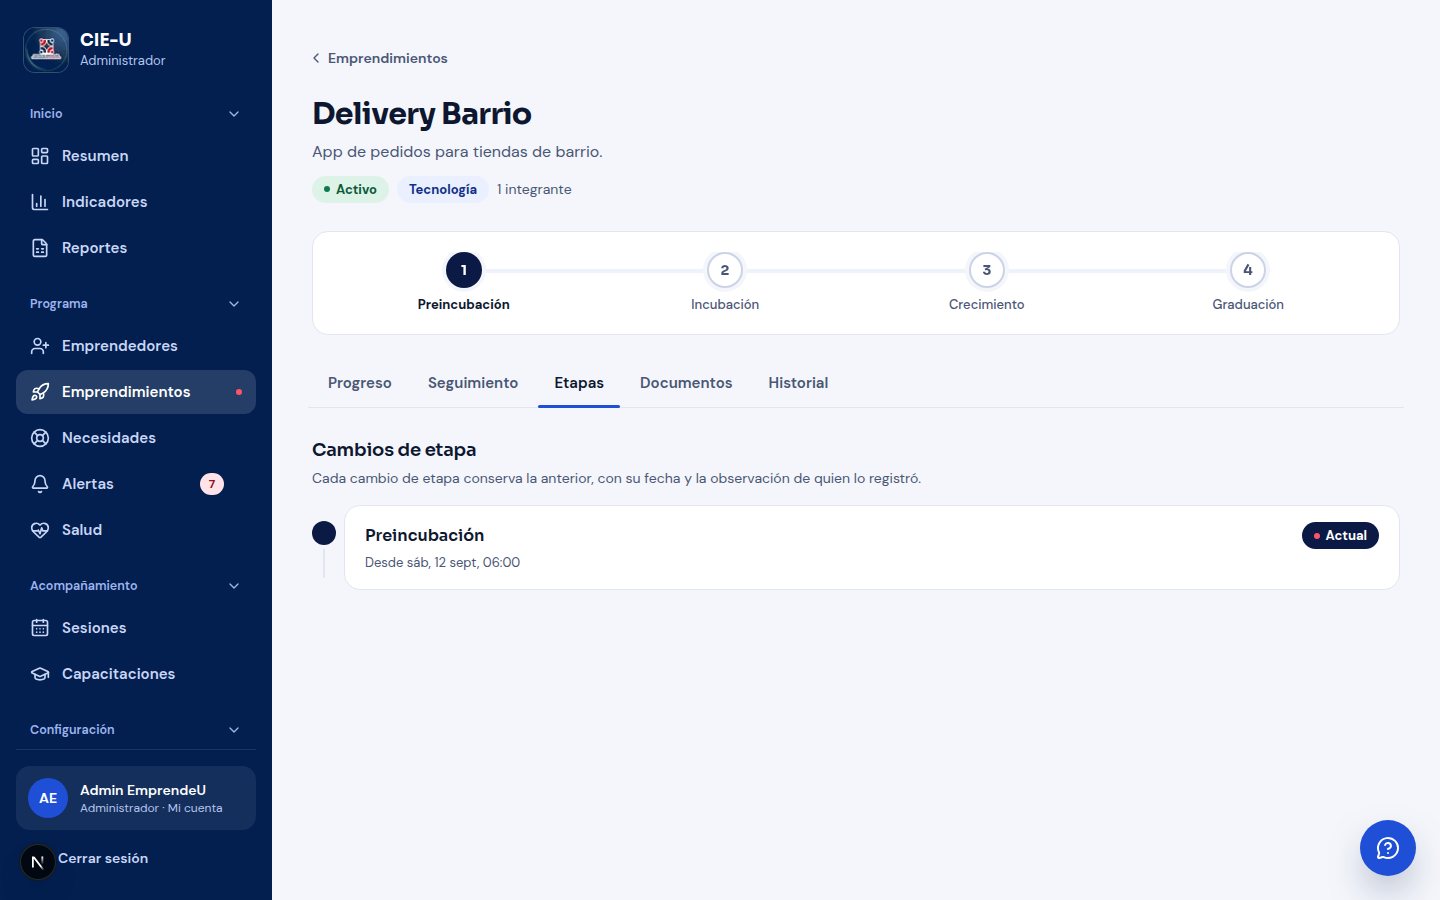
\includegraphics[width=0.97\textwidth,keepaspectratio]{imagenes/web_venture_stages.png}}
\par\vspace{3pt}\begin{flushleft}\small \textit{Nota.} Cada cambio conserva la etapa anterior.\end{flushleft}
\end{figure}

\begin{figure}[H]\singlespacing
\caption{Pestaña Documentos}\label{fig:web_venture_documents}
\centering\fbox{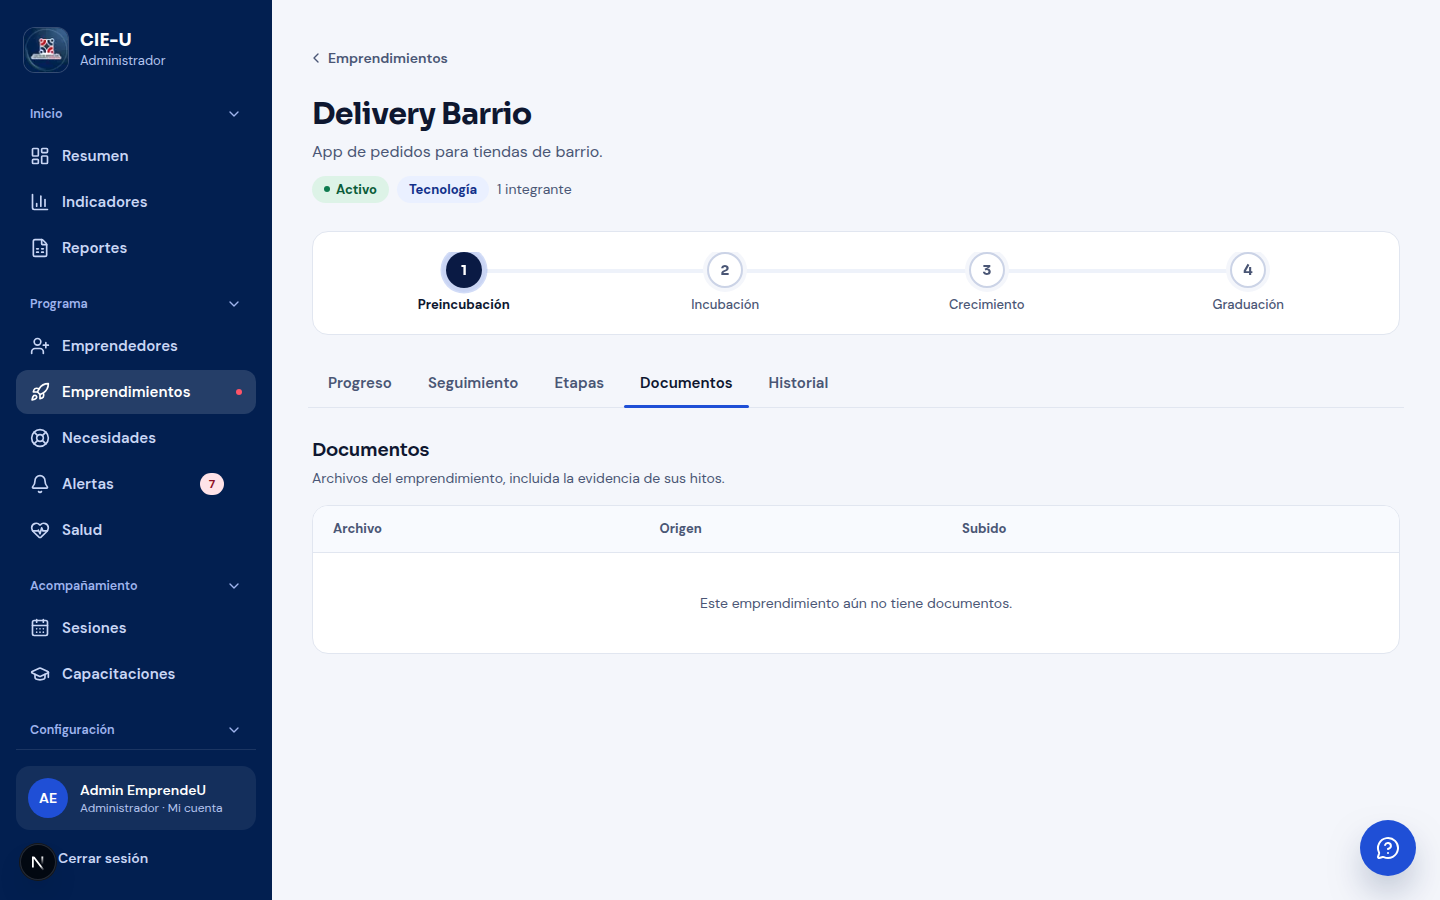
\includegraphics[width=0.97\textwidth,keepaspectratio]{imagenes/web_venture_documents.png}}
\par\vspace{3pt}\begin{flushleft}\small \textit{Nota.} Se distinguen documentos generales y evidencia de hito.\end{flushleft}
\end{figure}

\begin{figure}[H]\singlespacing
\caption{Pestaña Historial}\label{fig:web_venture_history}
\centering\fbox{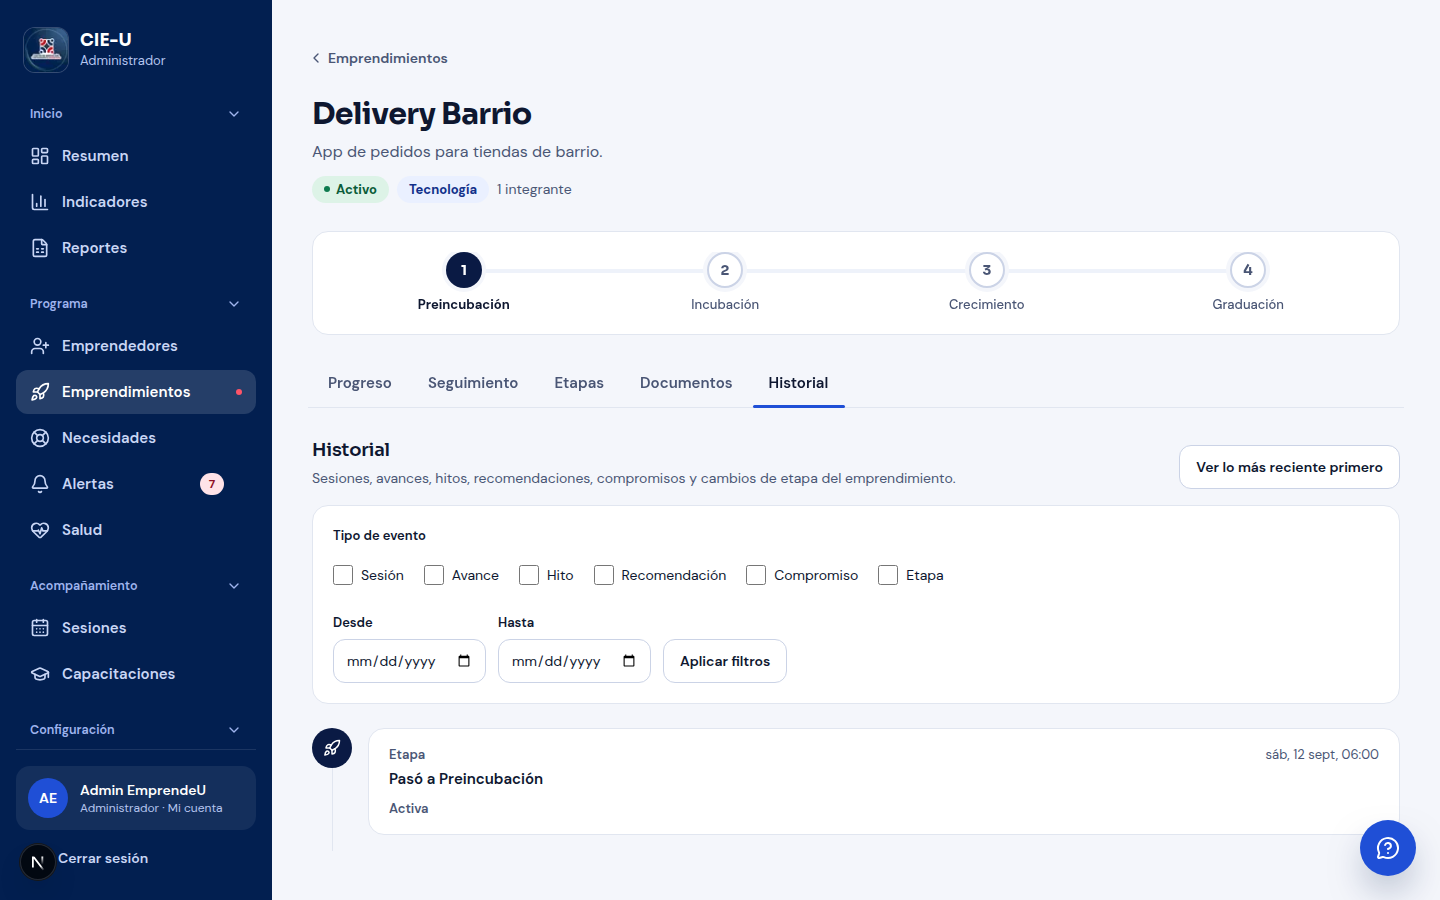
\includegraphics[width=0.97\textwidth,keepaspectratio]{imagenes/web_venture_history.png}}
\par\vspace{3pt}\begin{flushleft}\small \textit{Nota.} Se puede ordenar del más reciente al más antiguo.\end{flushleft}
\end{figure}

\textbf{Errores de documentos.} «Elige un archivo.», «Formato no permitido. Usa: \ldots{}», «El archivo supera N MB.».

\subsubsection*{5.2.5. Necesidades}

\addcontentsline{toc}{subsubsection}{5.2.5. Necesidades}

\textbf{Descripción.} Muestra las necesidades y dificultades que reportan los emprendedores. Las abiertas aparecen primero.

\begin{enumerate}
\item Abrir «Necesidades» y filtrar por estado y tipo.
\item Con permiso de modificación de seguimiento, seleccionar la acción de resolver en la fila.
\item El sistema confirma «Resuelta: \ldots{} Registrado en auditoría.».
\end{enumerate}

\begin{figure}[H]\singlespacing
\caption{Necesidades y dificultades}\label{fig:web_admin_needs}
\centering\fbox{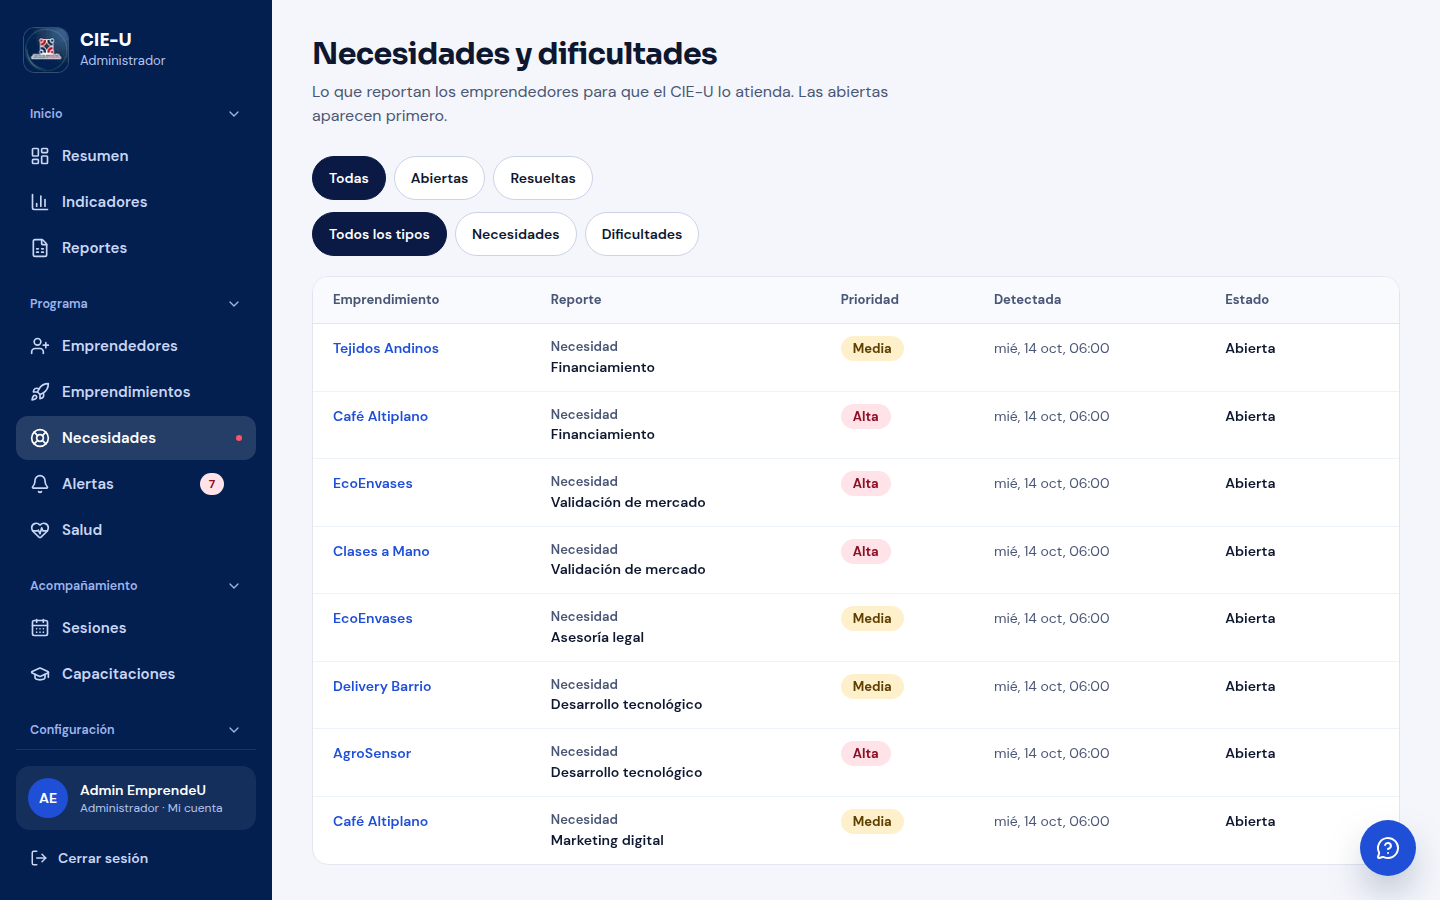
\includegraphics[width=0.97\textwidth,keepaspectratio]{imagenes/web_admin_needs.png}}
\par\vspace{3pt}\begin{flushleft}\small \textit{Nota.} La prioridad se muestra como Alta, Media o Baja.\end{flushleft}
\end{figure}

\subsubsection*{5.2.6. Alertas}

\addcontentsline{toc}{subsubsection}{5.2.6. Alertas}

\textbf{Descripción.} Lista los riesgos detectados: inactividad, caída de sentimiento y compromiso vencido. Una alerta no cambia el estado del emprendimiento.

\begin{enumerate}
\item Abrir «Alertas» y filtrar por estado (Todas, Abiertas, Revisadas, Atendidas, Descartadas) o por tipo.
\item Abrir una alerta para ver el motivo, la prioridad y la fecha de detección.
\item Con permiso de registro de seguimiento, registrar el seguimiento: la alerta pasa de abierta a revisada y luego a atendida o descartada.
\end{enumerate}

\begin{figure}[H]\singlespacing
\caption{Lista de alertas}\label{fig:web_admin_alerts}
\centering\fbox{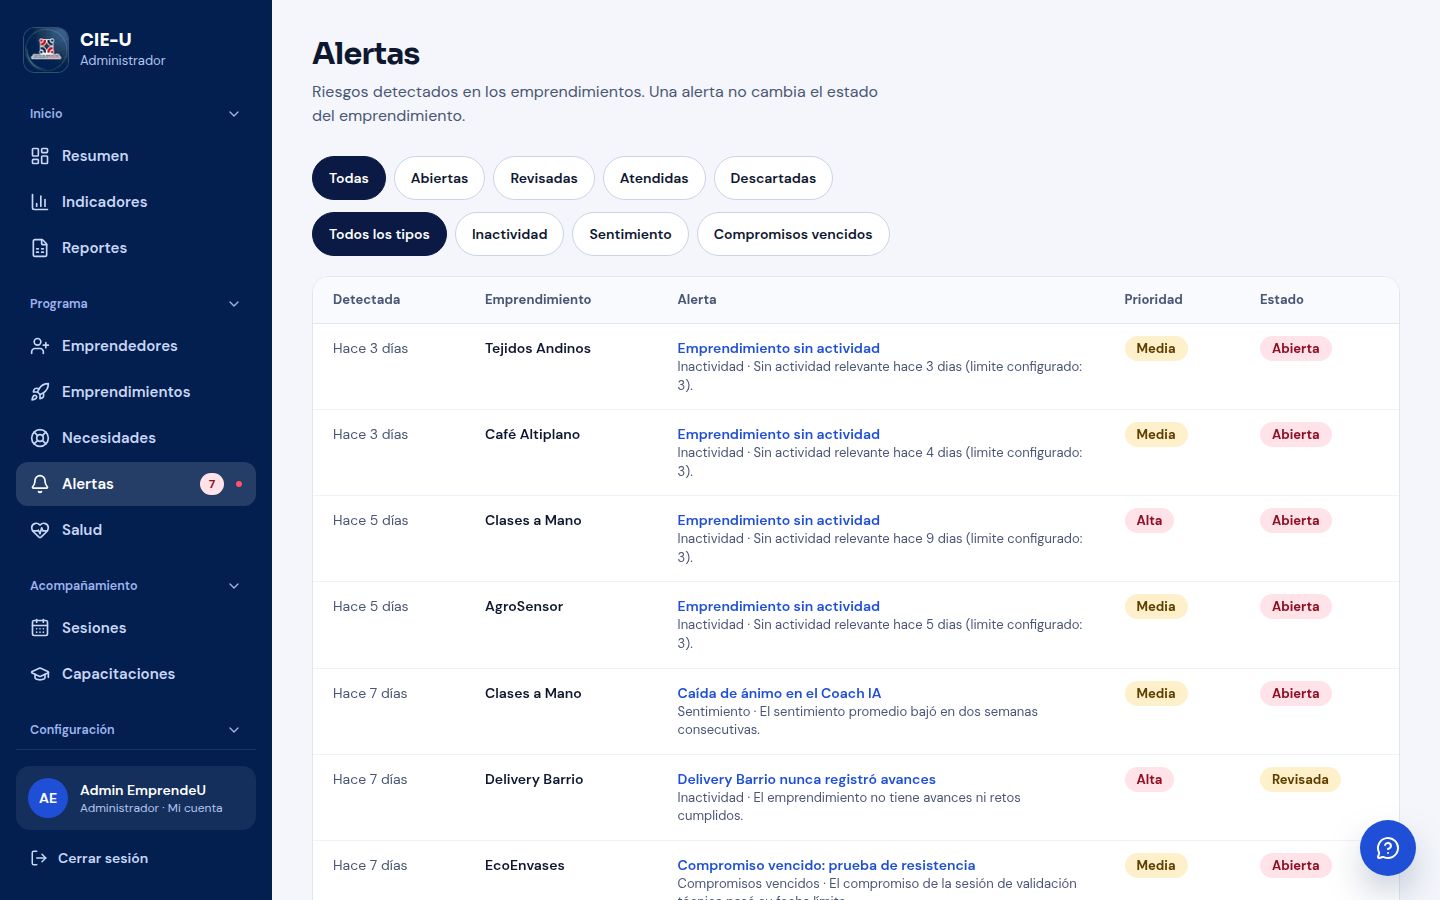
\includegraphics[width=0.97\textwidth,keepaspectratio]{imagenes/web_admin_alerts.png}}
\par\vspace{3pt}\begin{flushleft}\small \textit{Nota.} La cifra del menú indica las alertas abiertas.\end{flushleft}
\end{figure}

\begin{figure}[H]\singlespacing
\caption{Detalle de una alerta}\label{fig:web_alert_detail}
\centering\fbox{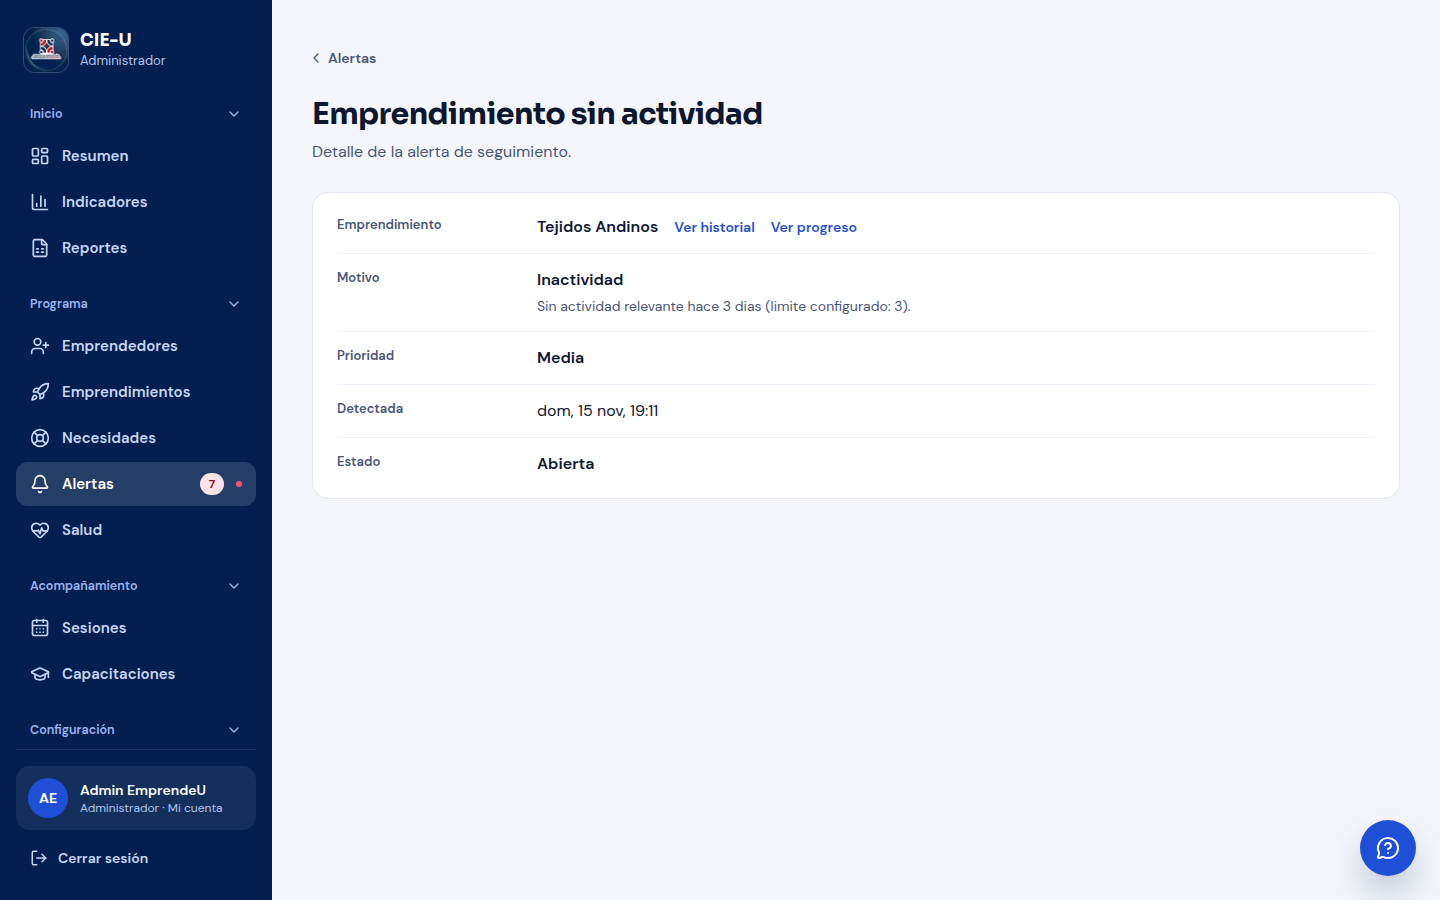
\includegraphics[width=0.97\textwidth,keepaspectratio]{imagenes/web_alert_detail.png}}
\par\vspace{3pt}\begin{flushleft}\small \textit{Nota.} Incluye enlaces al historial y al progreso del emprendimiento.\end{flushleft}
\end{figure}

Una alerta ya cerrada no admite nuevos cambios. El asesor ve solo las alertas de sus emprendimientos asignados.

\subsubsection*{5.2.7. Salud de los emprendimientos}

\addcontentsline{toc}{subsubsection}{5.2.7. Salud de los emprendimientos}

\textbf{Descripción.} Ordena los emprendimientos del más urgente al que mejor va. El puntaje combina alertas, compromisos vencidos, inactividad, tiempo en la etapa y ánimo en el coach. Verde equivale a 70 o más, ámbar a 40–69 y rojo a menos de 40.

\begin{figure}[H]\singlespacing
\caption{Salud de los emprendimientos}\label{fig:web_admin_health}
\centering\fbox{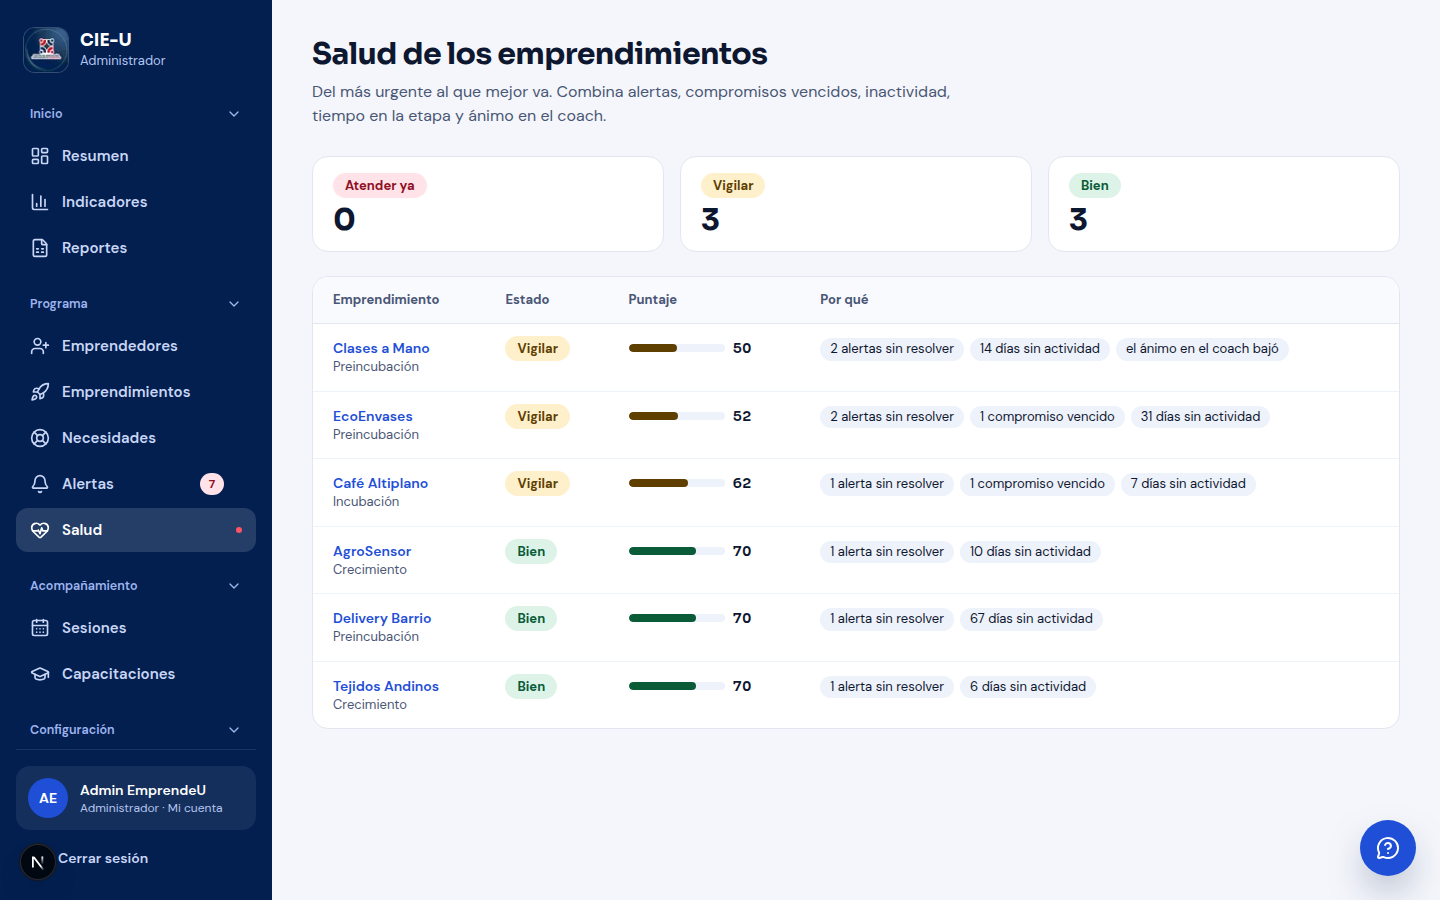
\includegraphics[width=0.97\textwidth,keepaspectratio]{imagenes/web_admin_health.png}}
\par\vspace{3pt}\begin{flushleft}\small \textit{Nota.} La columna «Por qué» explica el puntaje.\end{flushleft}
\end{figure}

\subsection*{5.3. Panel web: Acompañamiento}

\addcontentsline{toc}{subsection}{5.3. Panel web: Acompañamiento}

\subsubsection*{5.3.1. Asignaciones}

\addcontentsline{toc}{subsubsection}{5.3.1. Asignaciones}

\textbf{Descripción.} Habilita asesores y los asigna a emprendimientos. \textbf{Roles:} coordinación (permiso de registro de asesorías); el asesor solo consulta.

\begin{enumerate}
\item Abrir «Asignaciones».
\item En «Asesores», activar el interruptor de quien se habilita; solo los asesores habilitados pueden recibir asignaciones.
\item Seleccionar «Asignar asesor», elegir «Asesor» y «Emprendimiento».
\item Seleccionar «Confirmar asignación».
\end{enumerate}

\begin{figure}[H]\singlespacing
\caption{Asignaciones}\label{fig:web_admin_assignments}
\centering\fbox{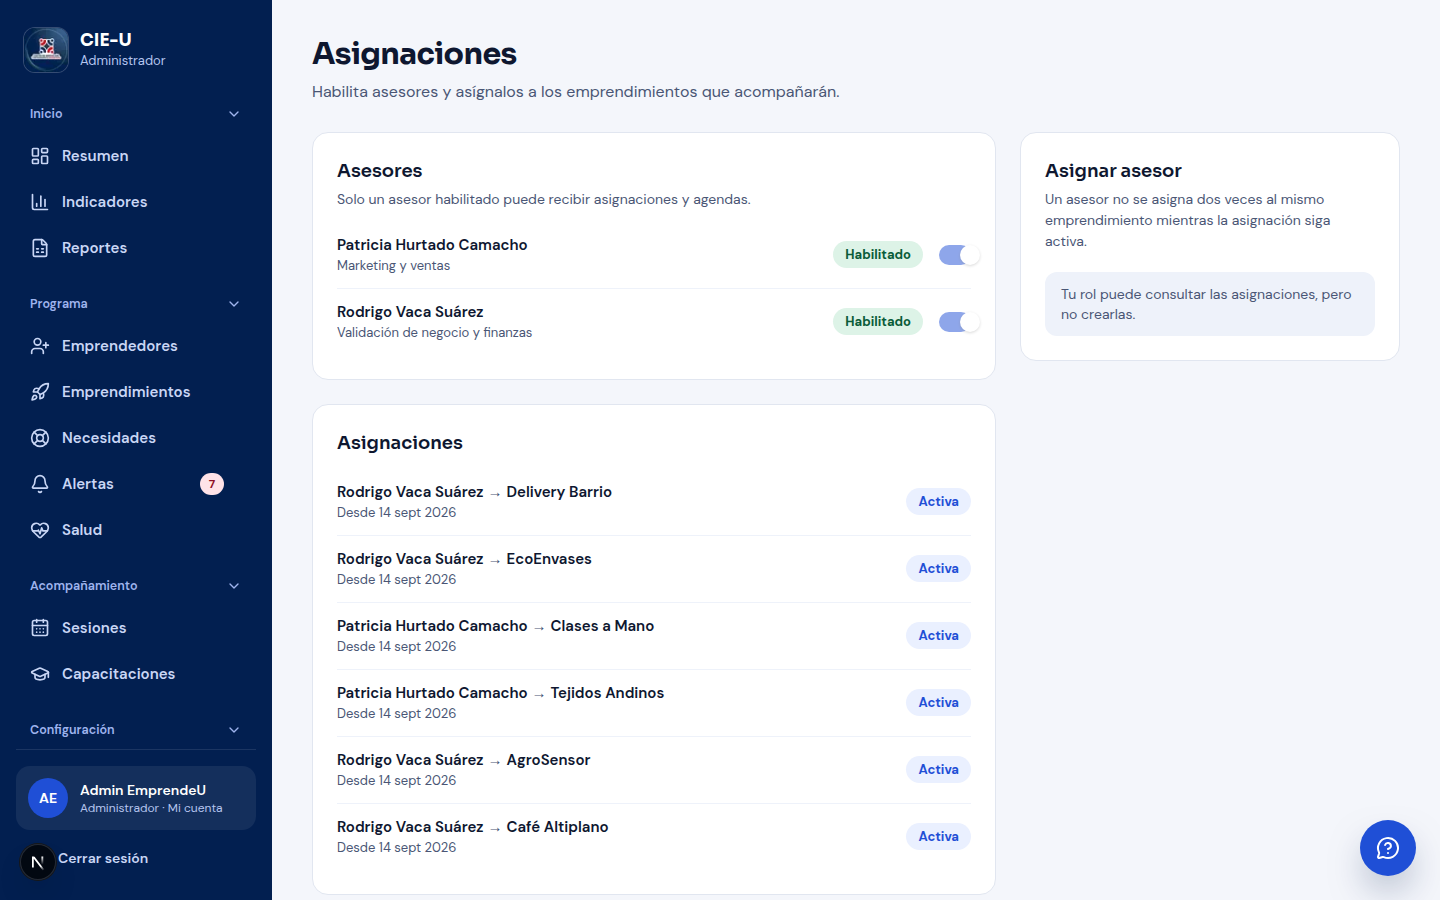
\includegraphics[width=0.97\textwidth,keepaspectratio]{imagenes/web_admin_assignments.png}}
\par\vspace{3pt}\begin{flushleft}\small \textit{Nota.} No se permite duplicar una asignación activa.\end{flushleft}
\end{figure}

\subsubsection*{5.3.2. Mi disponibilidad}

\addcontentsline{toc}{subsubsection}{5.3.2. Mi disponibilidad}

\textbf{Descripción.} El asesor define los horarios en los que atiende mentorías, en bloques de 60 minutos. Los emprendedores asignados agendan dentro de ellos.

\begin{enumerate}
\item Abrir «Mi disponibilidad».
\item En «Agregar horario», elegir «Día», «Desde» y «Hasta».
\item Seleccionar «Agregar horario».
\item Un horario puede bloquearse («Bloquear este horario»), volver a ofrecerse o eliminarse.
\end{enumerate}

\begin{figure}[H]\singlespacing
\caption{Disponibilidad del asesor}\label{fig:web_asesor_availability}
\centering\fbox{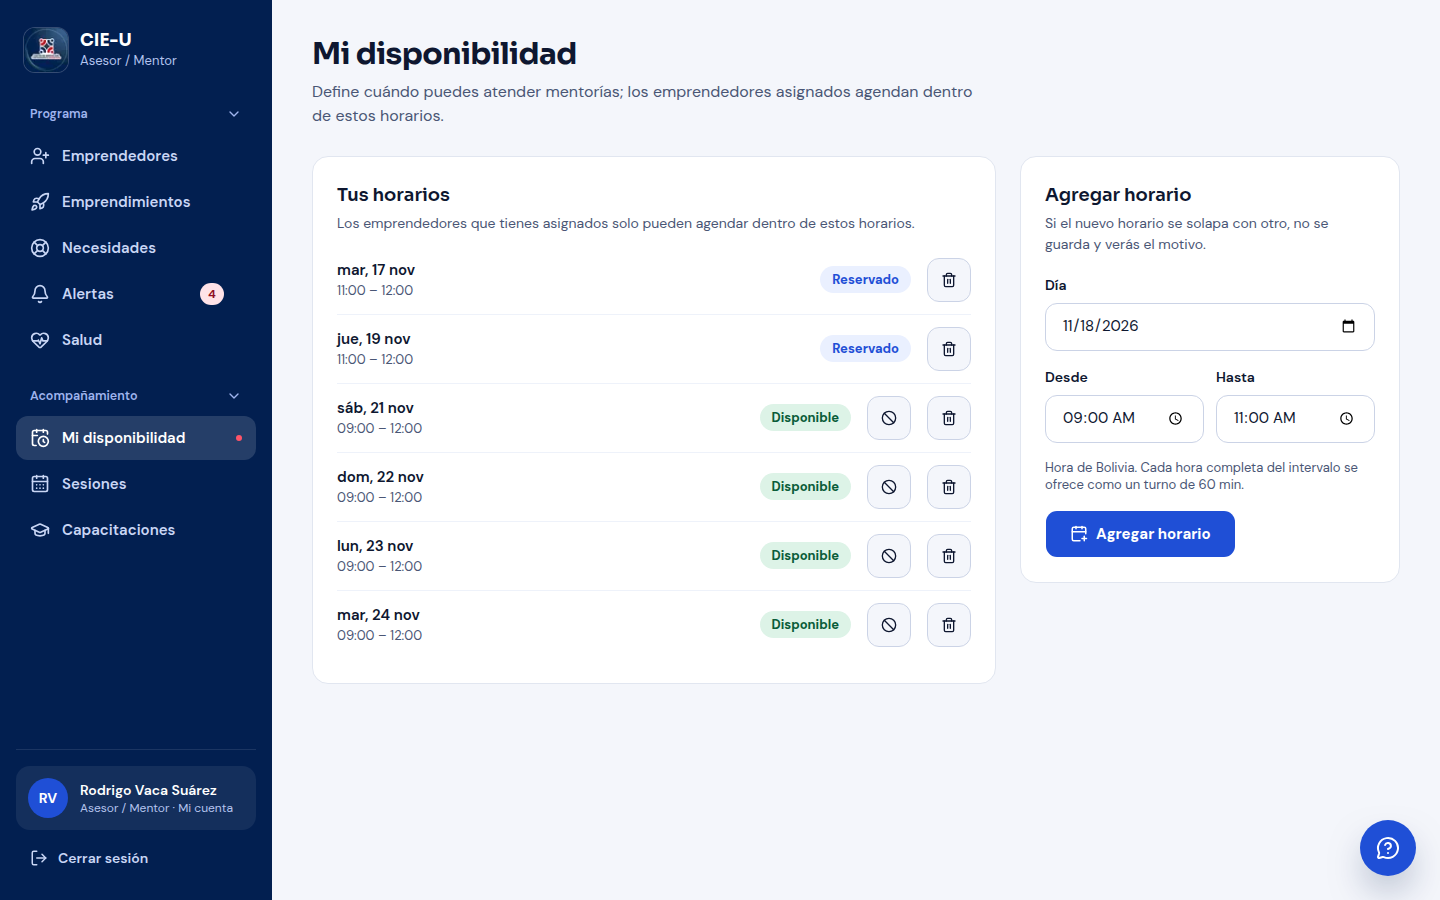
\includegraphics[width=0.97\textwidth,keepaspectratio]{imagenes/web_asesor_availability.png}}
\par\vspace{3pt}\begin{flushleft}\small \textit{Nota.} Los horarios reservados no pueden eliminarse.\end{flushleft}
\end{figure}

\textbf{Validaciones.} «Elige una fecha.», «Elige una hora.», «La hora de fin debe ser posterior al inicio.». Los horarios no pueden superponerse.

\subsubsection*{5.3.3. Sesiones}

\addcontentsline{toc}{subsubsection}{5.3.3. Sesiones}

\textbf{Descripción.} Lista las mentorías por estado (Programadas, Realizadas, Canceladas) y periodo, y permite registrar lo ocurrido. El asesor ve sus sesiones; el resto del personal ve todas.

\begin{enumerate}
\item Abrir «Sesiones» y aplicar los filtros.
\item \textbf{Registrar sesión realizada:} completar Emprendimiento, Tema, Fecha realizada, Hora, Modalidad (Presencial, Virtual, Híbrida) y Observaciones; seleccionar «Registrar sesión».
\item \textbf{Nueva recomendación:} escribir Título y Recomendación; seleccionar «Guardar recomendación».
\item \textbf{Nuevo compromiso:} elegir Responsable, escribir el Compromiso y, opcionalmente, la Fecha límite; seleccionar «Guardar compromiso». Si no hay fecha se usa el plazo de Parámetros.
\end{enumerate}

\begin{figure}[H]\singlespacing
\caption{Sesiones de mentoría}\label{fig:web_admin_sessions}
\centering\fbox{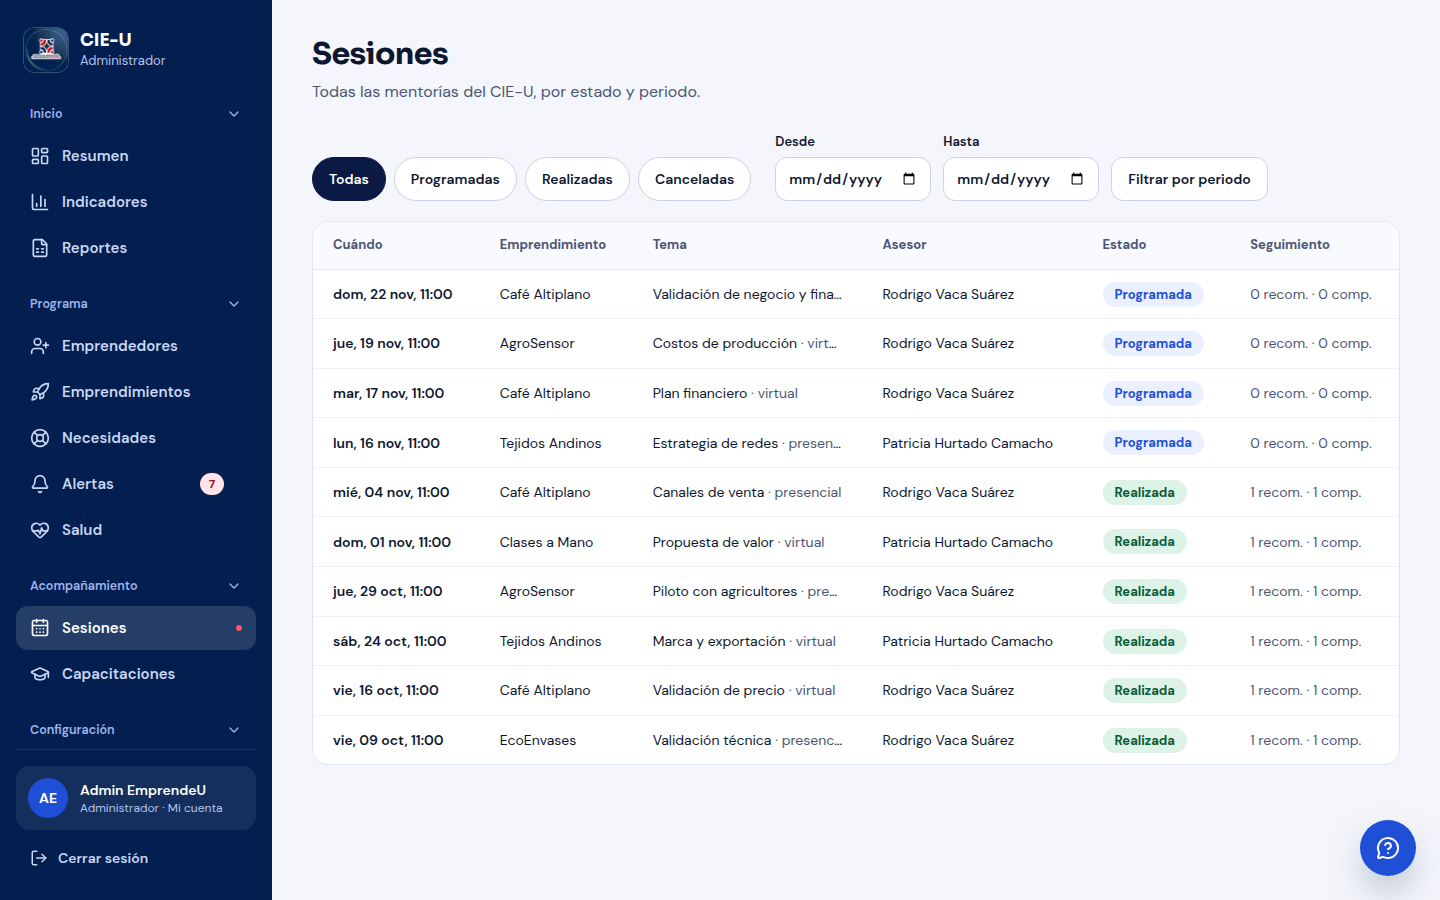
\includegraphics[width=0.97\textwidth,keepaspectratio]{imagenes/web_admin_sessions.png}}
\par\vspace{3pt}\begin{flushleft}\small \textit{Nota.} Se puede filtrar por estado y por fechas.\end{flushleft}
\end{figure}

\textbf{Restricciones.} Una sesión realizada no puede tener fecha futura. El asesor solo registra en emprendimientos que tiene asignados.

\subsubsection*{5.3.4. Capacitaciones}

\addcontentsline{toc}{subsubsection}{5.3.4. Capacitaciones}

\textbf{Descripción.} Gestiona talleres y charlas, sus participantes y la asistencia.

\begin{enumerate}
\item Abrir «Capacitaciones» y filtrar por estado.
\item \textbf{Crear:} «Nueva capacitación» $\rightarrow$ Título, Tipo, Modalidad, Día, Hora, Estado y Descripción $\rightarrow$ «Crear capacitación».
\item \textbf{Editar:} «Editar capacitación» $\rightarrow$ «Guardar cambios».
\item \textbf{Participantes:} abrir la capacitación, buscar con «Buscar emprendedor» y seleccionar «Agregar participante».
\item \textbf{Asistencia:} registrar la asistencia o la ausencia de cada participante desde el panel de participantes.
\end{enumerate}

\begin{figure}[H]\singlespacing
\caption{Lista de capacitaciones}\label{fig:web_admin_training}
\centering\fbox{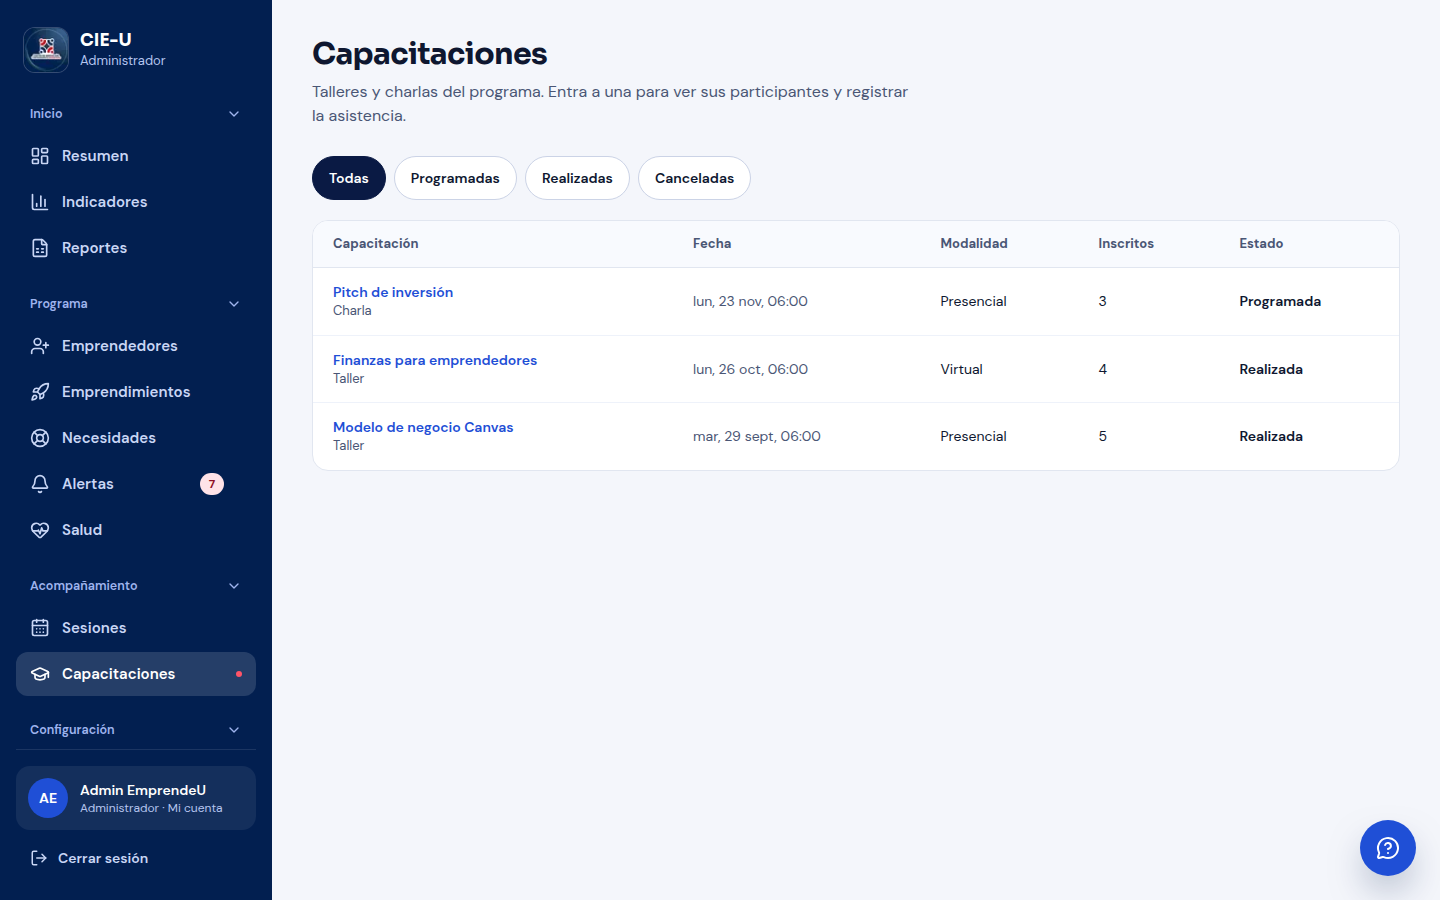
\includegraphics[width=0.97\textwidth,keepaspectratio]{imagenes/web_admin_training.png}}
\par\vspace{3pt}\begin{flushleft}\small \textit{Nota.} Muestra fecha, modalidad, estado e inscritos.\end{flushleft}
\end{figure}

\begin{figure}[H]\singlespacing
\caption{Detalle de una capacitación}\label{fig:web_training_detail}
\centering\fbox{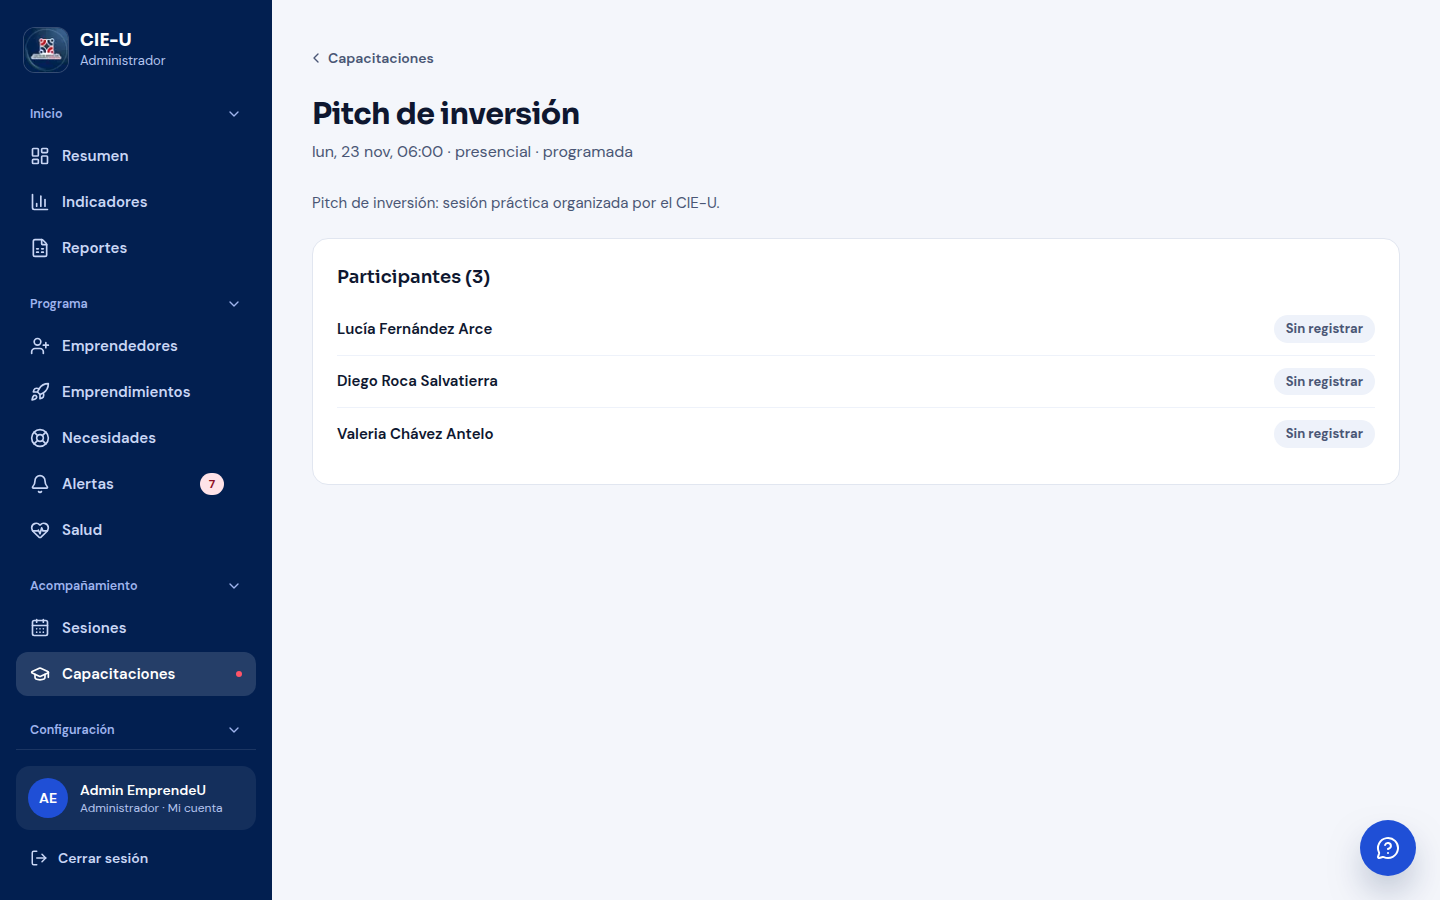
\includegraphics[width=0.97\textwidth,keepaspectratio]{imagenes/web_training_detail.png}}
\par\vspace{3pt}\begin{flushleft}\small \textit{Nota.} La asistencia se registra por participante.\end{flushleft}
\end{figure}

Una capacitación cancelada ya no admite participantes, y un emprendedor no puede repetirse en la misma capacitación.

\subsection*{5.4. Panel web: Configuración}

\addcontentsline{toc}{subsection}{5.4. Panel web: Configuración}

\subsubsection*{5.4.1. Usuarios}

\addcontentsline{toc}{subsubsection}{5.4.1. Usuarios}

\textbf{Descripción.} Gestiona las cuentas de la plataforma. \textbf{Roles:} administrador.

\begin{enumerate}
\item Abrir «Usuarios». Buscar por nombre o correo y filtrar por rol.
\item \textbf{Crear:} «Nuevo usuario» $\rightarrow$ «Nombre y apellidos», «Correo», «Rol asignado» $\rightarrow$ crear y copiar la «Contraseña temporal».
\item \textbf{Habilitar o deshabilitar:} usar el interruptor de «Estado de la cuenta».
\item \textbf{Cambiar el rol:} elegir el nuevo rol en la columna de rol.
\end{enumerate}

\begin{figure}[H]\singlespacing
\caption{Lista de usuarios}\label{fig:web_admin_users}
\centering\fbox{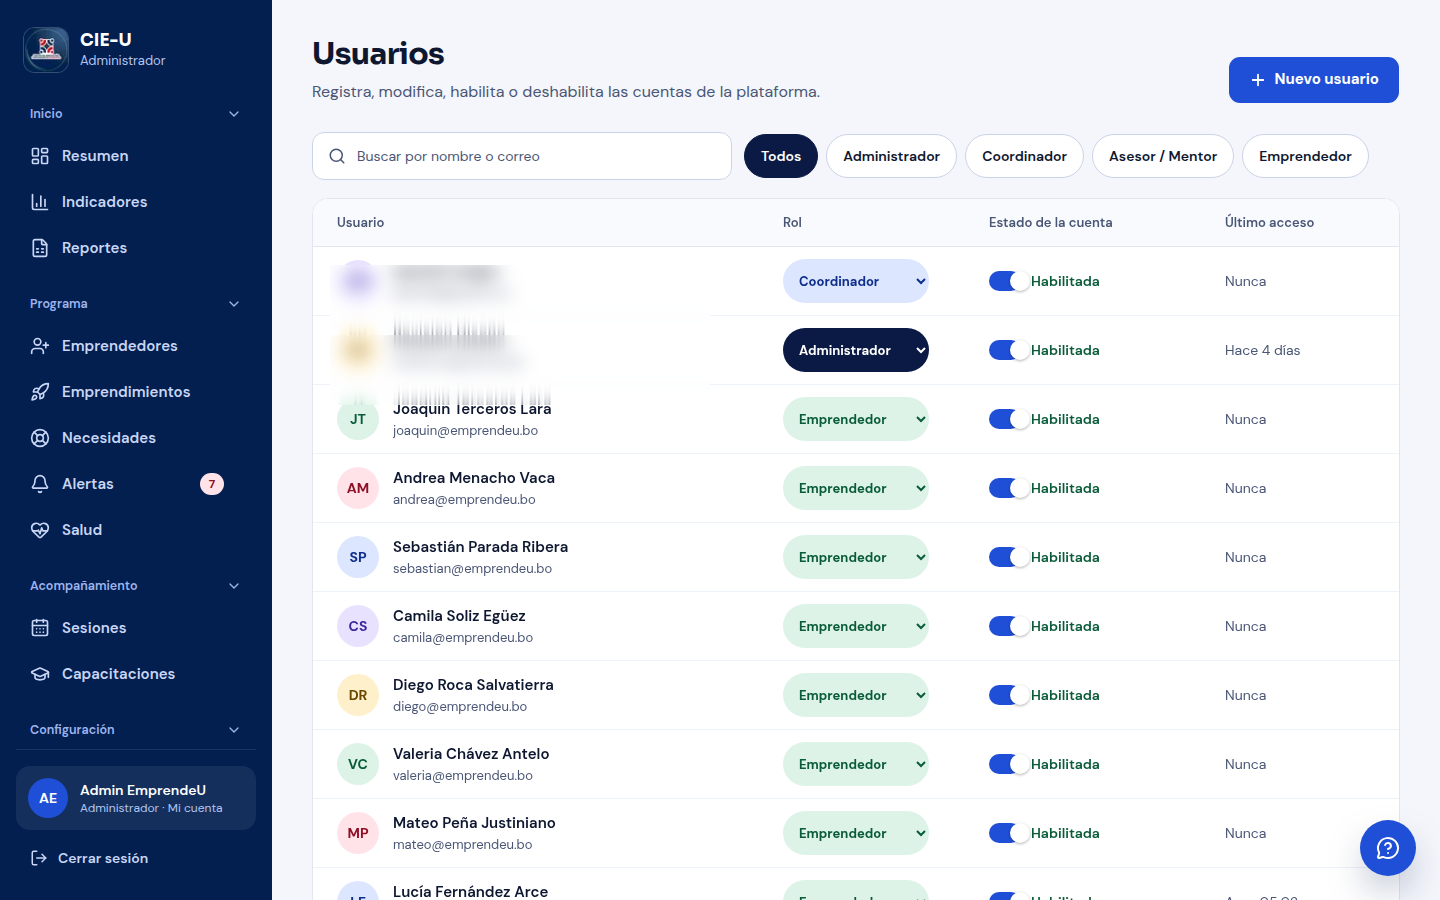
\includegraphics[width=0.97\textwidth,keepaspectratio]{imagenes/web_admin_users.png}}
\par\vspace{3pt}\begin{flushleft}\small \textit{Nota.} Se difuminaron datos personales no pertenecientes a la demostración.\end{flushleft}
\end{figure}

\textbf{Validaciones.} «Ingresa nombre y apellido.», «Ya existe una cuenta con ese correo.».

\subsubsection*{5.4.2. Roles y permisos}

\addcontentsline{toc}{subsubsection}{5.4.2. Roles y permisos}

\textbf{Descripción.} Muestra la matriz de siete módulos por cuatro acciones y permite editarla (permiso administrativo de usuarios).

\begin{enumerate}
\item Abrir «Roles y permisos» y seleccionar un rol.
\item Marcar o desmarcar las casillas y seleccionar «Guardar cambios». Los cambios rigen de inmediato.
\item \textbf{Nuevo rol:} «Nuevo rol» $\rightarrow$ nombre (mínimo 3 caracteres) y plantilla («Sin permisos» o «Solo lectura»).
\item Los roles personalizados pueden editarse o eliminarse. Un rol con usuarios no puede eliminarse: «Reasigna a sus usuarios antes de eliminarlo».
\end{enumerate}

\begin{figure}[H]\singlespacing
\caption{Roles y permisos}\label{fig:web_admin_roles}
\centering\fbox{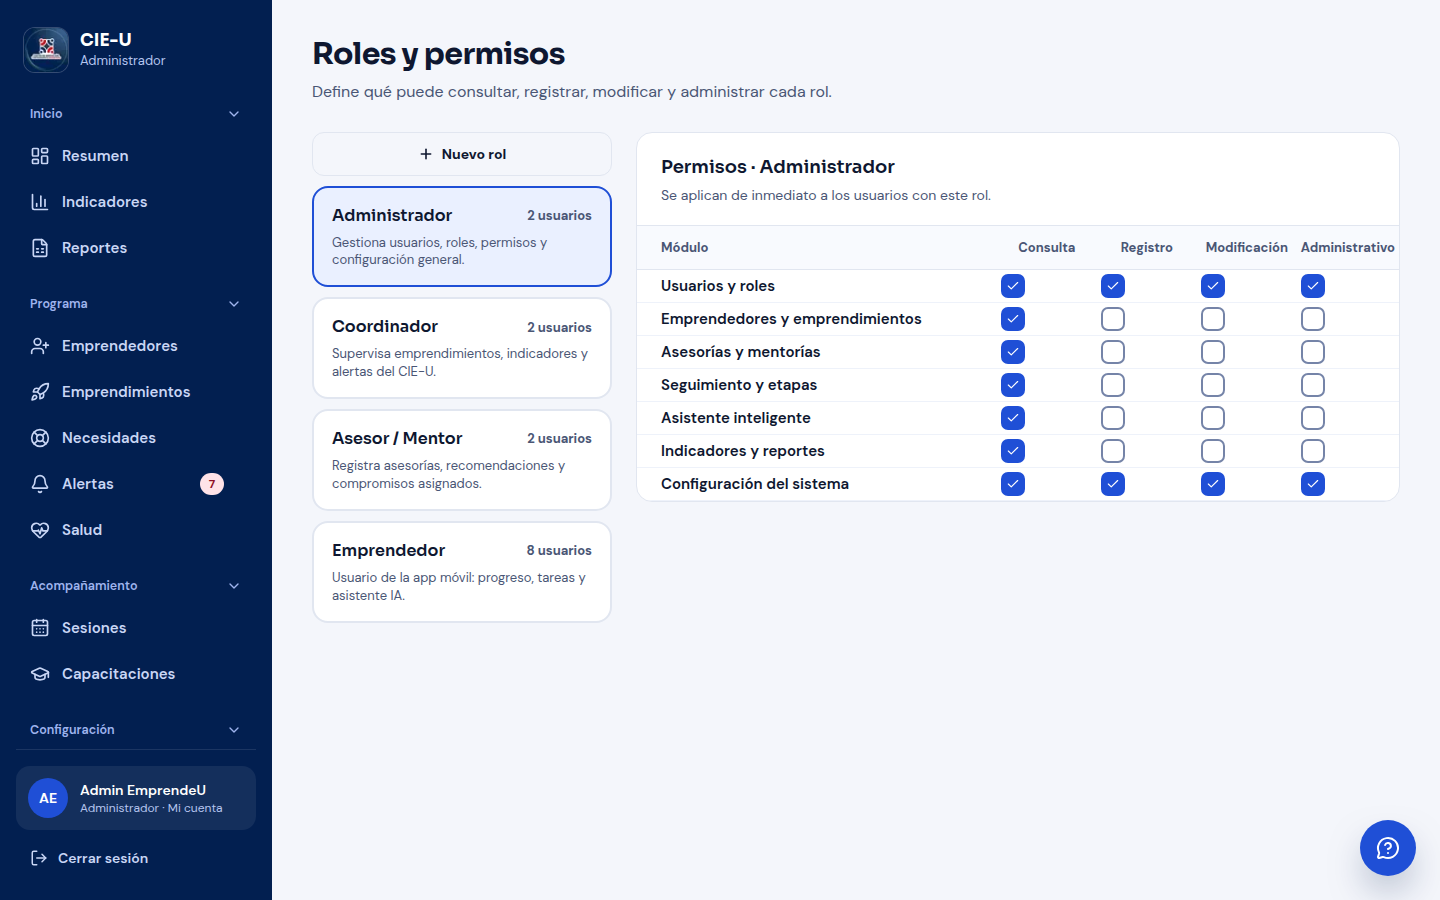
\includegraphics[width=0.97\textwidth,keepaspectratio]{imagenes/web_admin_roles.png}}
\par\vspace{3pt}\begin{flushleft}\small \textit{Nota.} Los cuatro roles del sistema no pueden renombrarse ni eliminarse.\end{flushleft}
\end{figure}

\subsubsection*{5.4.3. Parámetros de seguimiento}

\addcontentsline{toc}{subsubsection}{5.4.3. Parámetros de seguimiento}

\textbf{Descripción.} Reglas que usa el sistema para detectar inactividad y riesgo de deserción: «Periodo de inactividad», «Periodos consecutivos para activar», «Caída del índice de sentimiento», «Plazo de los compromisos» e «Incumplimiento de compromisos», con los interruptores «Notificar al asesor asignado», «Notificar al Coordinador del CIE-U» y «Alertas activas».

\begin{enumerate}
\item Abrir «Parámetros».
\item Ajustar los valores y revisar el resumen de la derecha.
\item Guardar. El sistema confirma «Parámetros de seguimiento actualizados. Registrado en auditoría.».
\end{enumerate}

\begin{figure}[H]\singlespacing
\caption{Parámetros de seguimiento}\label{fig:web_admin_settings}
\centering\fbox{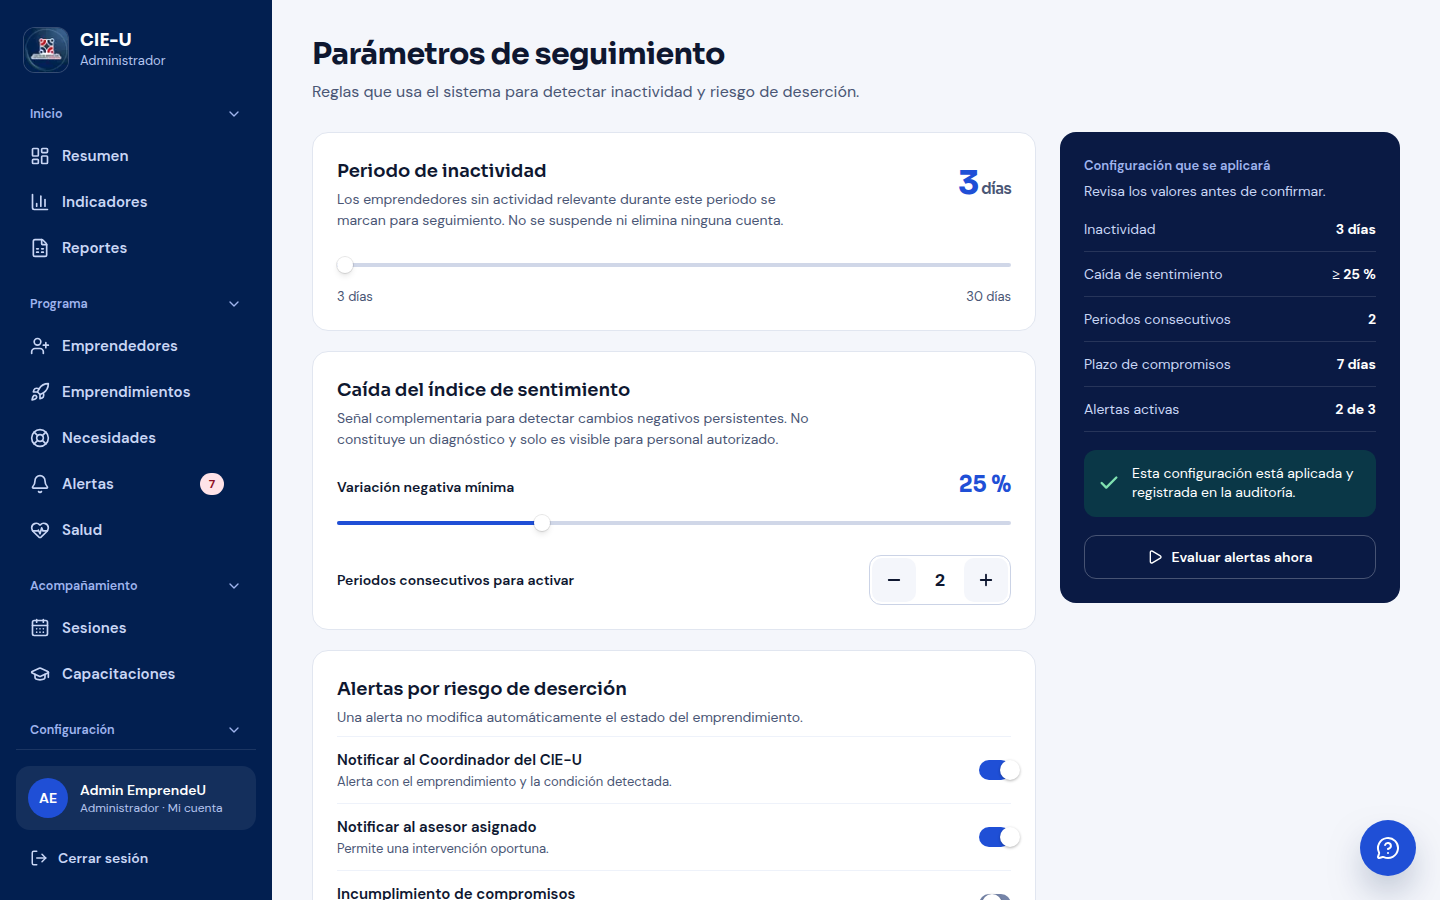
\includegraphics[width=0.97\textwidth,keepaspectratio]{imagenes/web_admin_settings.png}}
\par\vspace{3pt}\begin{flushleft}\small \textit{Nota.} El botón «Evaluar alertas ahora» requiere permiso administrativo.\end{flushleft}
\end{figure}

\subsubsection*{5.4.4. Catálogos y XP}

\addcontentsline{toc}{subsubsection}{5.4.4. Catálogos y XP}

\textbf{Descripción.} Administra las etapas del ciclo de vida, los retos con sus recompensas de XP y las insignias, en tres pestañas: Etapas, Retos e Insignias. Activar o desactivar una etapa y editar el XP de un reto requiere permiso de modificación de configuración.

\begin{figure}[H]\singlespacing
\caption{Catálogos y gamificación}\label{fig:web_admin_catalogs}
\centering\fbox{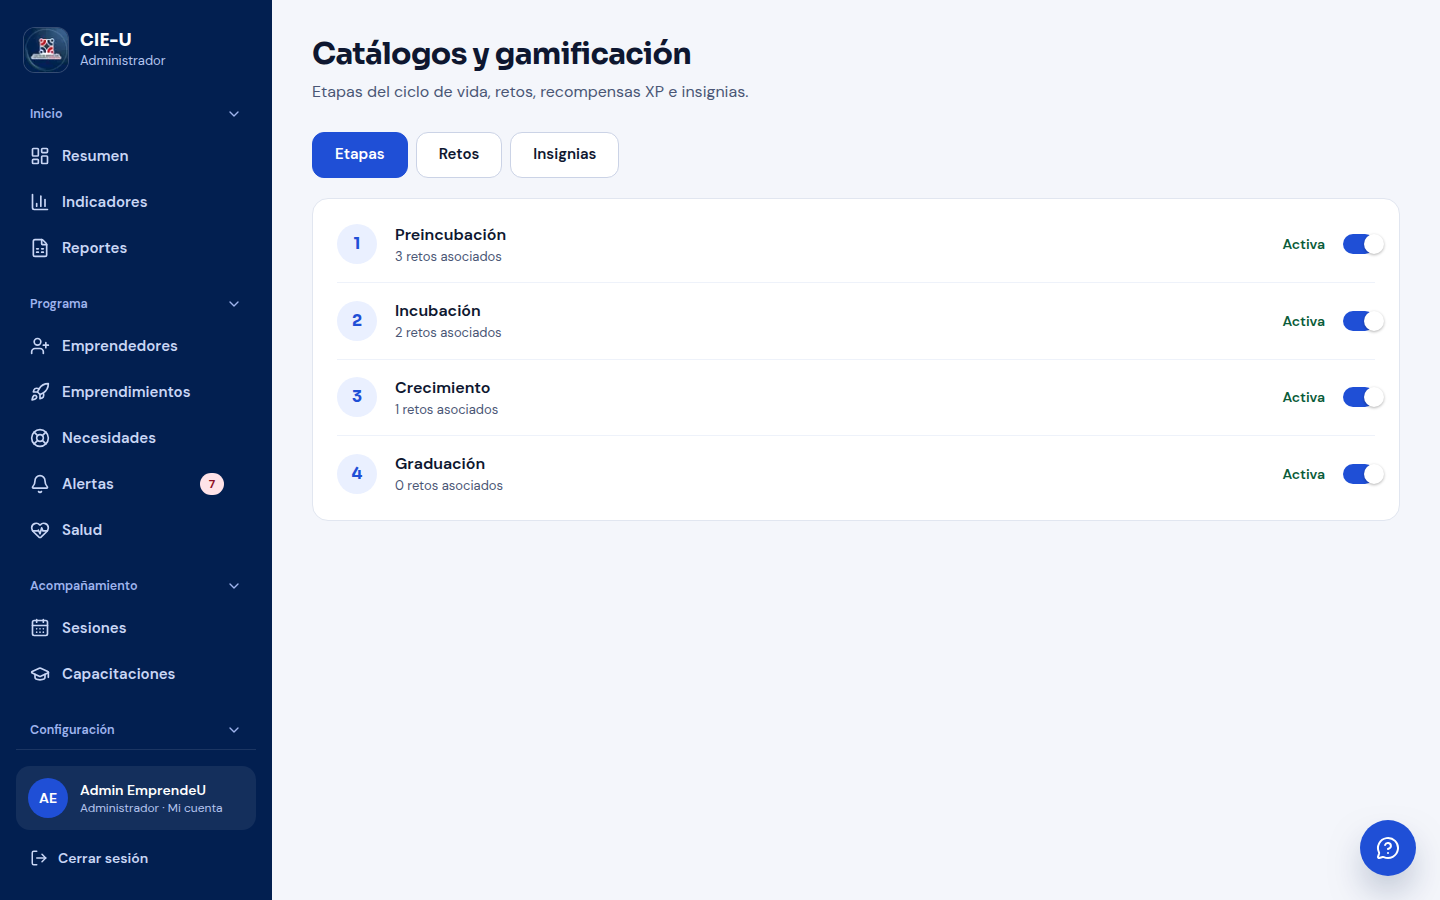
\includegraphics[width=0.97\textwidth,keepaspectratio]{imagenes/web_admin_catalogs.png}}
\par\vspace{3pt}\begin{flushleft}\small \textit{Nota.} Cada etapa indica cuántos retos tiene asociados.\end{flushleft}
\end{figure}

\subsubsection*{5.4.5. Base de conocimiento}

\addcontentsline{toc}{subsubsection}{5.4.5. Base de conocimiento}

\textbf{Descripción.} Documentos con los que responde el coach de IA. Solo los activos se utilizan.

\begin{enumerate}
\item Abrir «Base de conocimiento».
\item Seleccionar «Subir documento» y elegir el archivo (.txt, .md, .pdf o .docx, de hasta 10 MB).
\item Completar Título, Fuente y Descripción (opcionales) y seleccionar «Subir y procesar».
\item El documento pasa por los estados Procesando, Activo o Error. Un documento activo puede desactivarse.
\end{enumerate}

\begin{figure}[H]\singlespacing
\caption{Base de conocimiento}\label{fig:web_admin_knowledge}
\centering\fbox{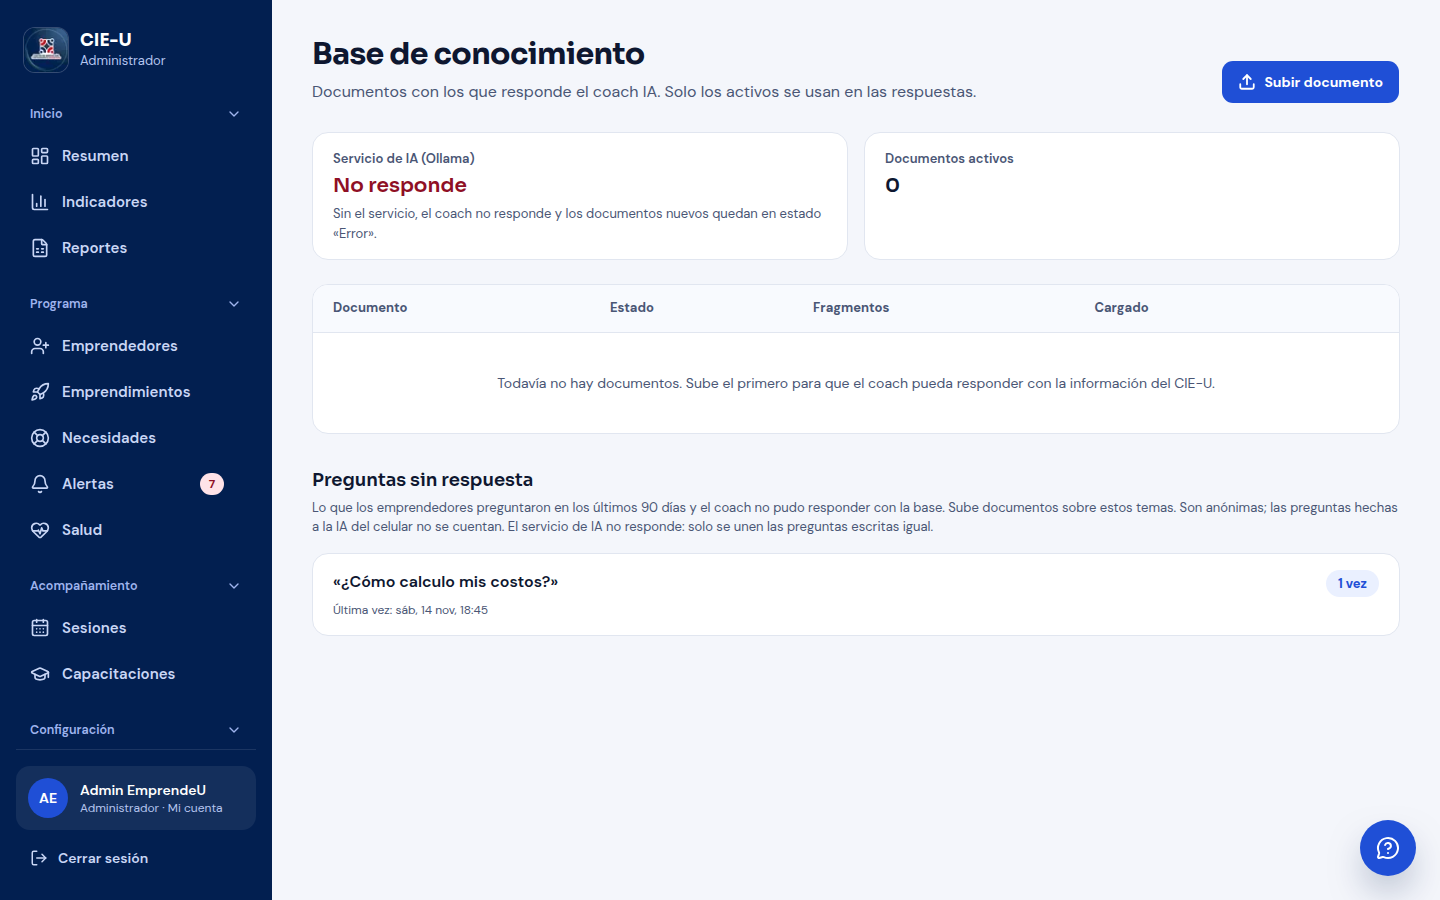
\includegraphics[width=0.97\textwidth,keepaspectratio]{imagenes/web_admin_knowledge.png}}
\par\vspace{3pt}\begin{flushleft}\small \textit{Nota.} En el momento de la captura el servicio de IA aparecía como «No responde».\end{flushleft}
\end{figure}

La sección «Preguntas sin respuesta» lista, de forma anónima, las consultas que el coach no pudo resolver.

\subsubsection*{5.4.6. Auditoría}

\addcontentsline{toc}{subsubsection}{5.4.6. Auditoría}

\textbf{Descripción.} Registro de acciones sensibles: hora, actor, acción y resultado (Exitoso o Rechazado).

\begin{enumerate}
\item Abrir «Auditoría».
\item Filtrar por categoría (Usuarios, Roles, Configuración, Accesos, Negocio).
\item Seleccionar «Exportar CSV» para descargar el registro filtrado.
\end{enumerate}

\begin{figure}[H]\singlespacing
\caption{Auditoría}\label{fig:web_admin_audit}
\centering\fbox{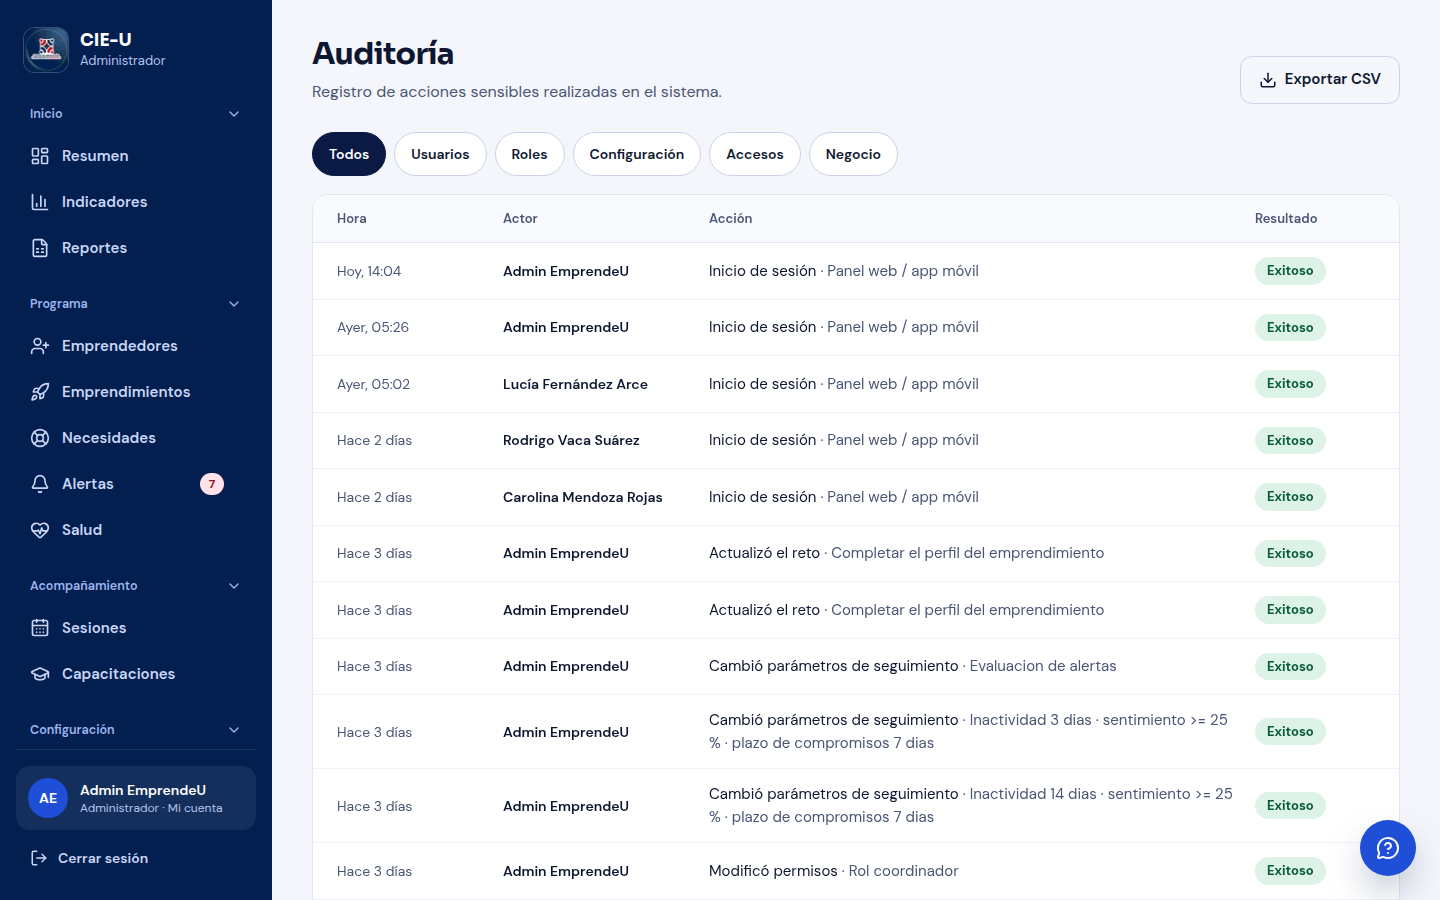
\includegraphics[width=0.97\textwidth,keepaspectratio]{imagenes/web_admin_audit.png}}
\par\vspace{3pt}\begin{flushleft}\small \textit{Nota.} El actor aparece como «Sistema» cuando la acción es automática.\end{flushleft}
\end{figure}

\subsubsection*{5.4.7. Mi cuenta}

\addcontentsline{toc}{subsubsection}{5.4.7. Mi cuenta}

\textbf{Descripción.} Muestra los datos de la sesión y permite cambiar la contraseña. Está disponible para todo el personal.

\begin{enumerate}
\item Abrir «Mi cuenta».
\item Escribir la contraseña actual, la nueva y su confirmación.
\item Seleccionar «Cambiar contraseña».
\item El sistema confirma y cierra las demás sesiones abiertas con la contraseña anterior.
\end{enumerate}

\begin{figure}[H]\singlespacing
\caption{Mi cuenta}\label{fig:web_admin_account}
\centering\fbox{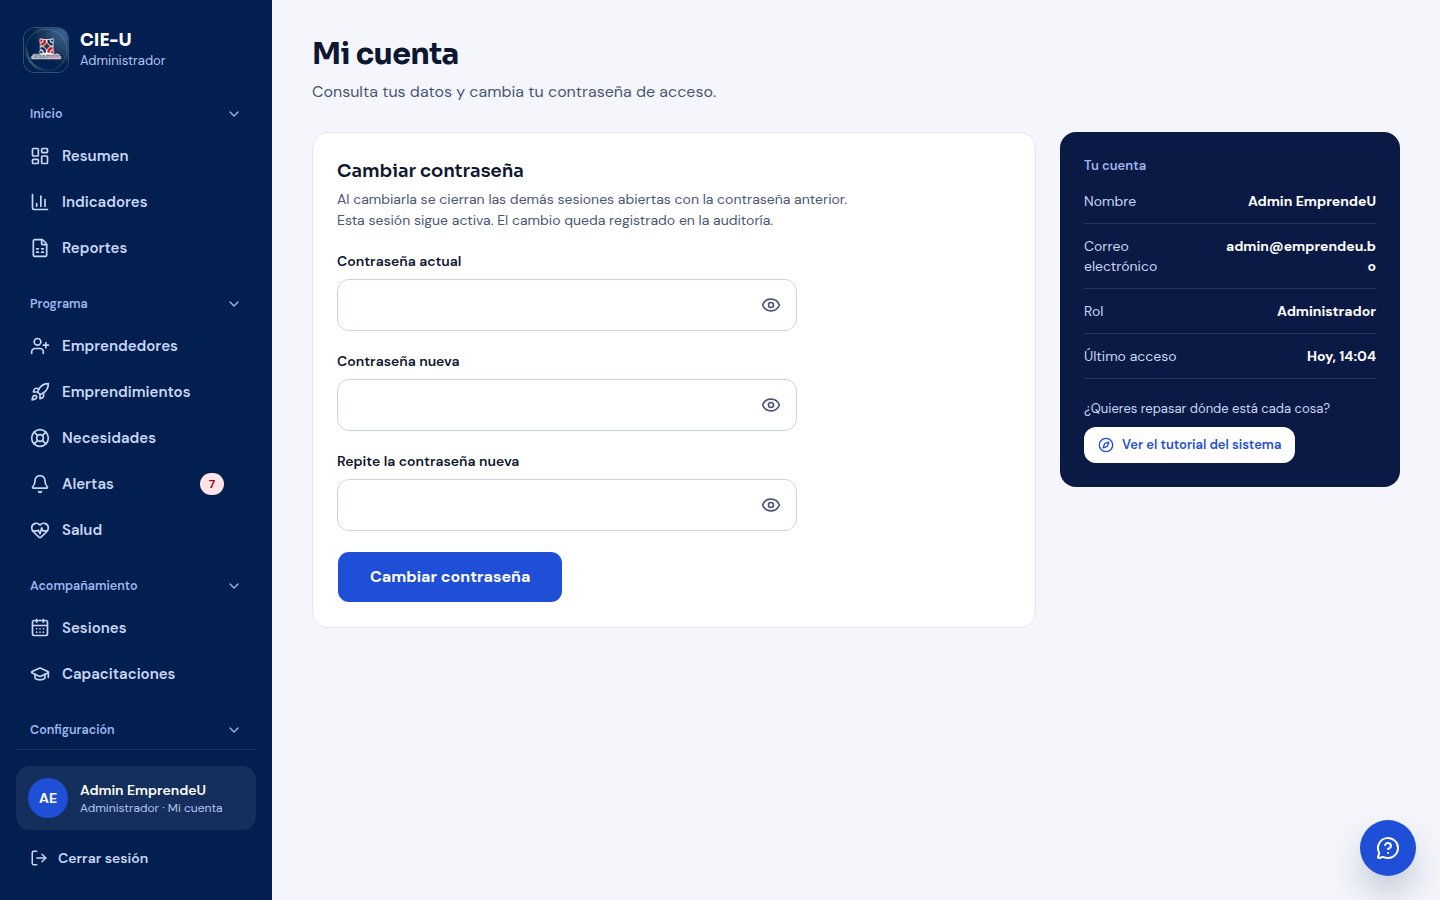
\includegraphics[width=0.97\textwidth,keepaspectratio]{imagenes/web_admin_account.png}}
\par\vspace{3pt}\begin{flushleft}\small \textit{Nota.} Incluye el botón «Ver el tutorial del sistema».\end{flushleft}
\end{figure}

\textbf{Validaciones.} «La contraseña actual no es correcta.», «La contraseña nueva debe ser distinta de la actual.», «Las contraseñas no coinciden.».

\subsection*{5.5. Panel web: ayuda y tutorial}

\addcontentsline{toc}{subsection}{5.5. Panel web: ayuda y tutorial}

\textbf{Tutorial guiado.} Aparece en el primer ingreso (Figura~\ref{fig:web_tutorial_inicio}) con los botones «Saltar tutorial» y «Comenzar recorrido». Recorre el menú según los permisos de la persona. Puede repetirse desde «Mi cuenta» con «Ver el tutorial del sistema».

\begin{figure}[H]\singlespacing
\caption{Tutorial del primer ingreso}\label{fig:web_tutorial_inicio}
\centering\fbox{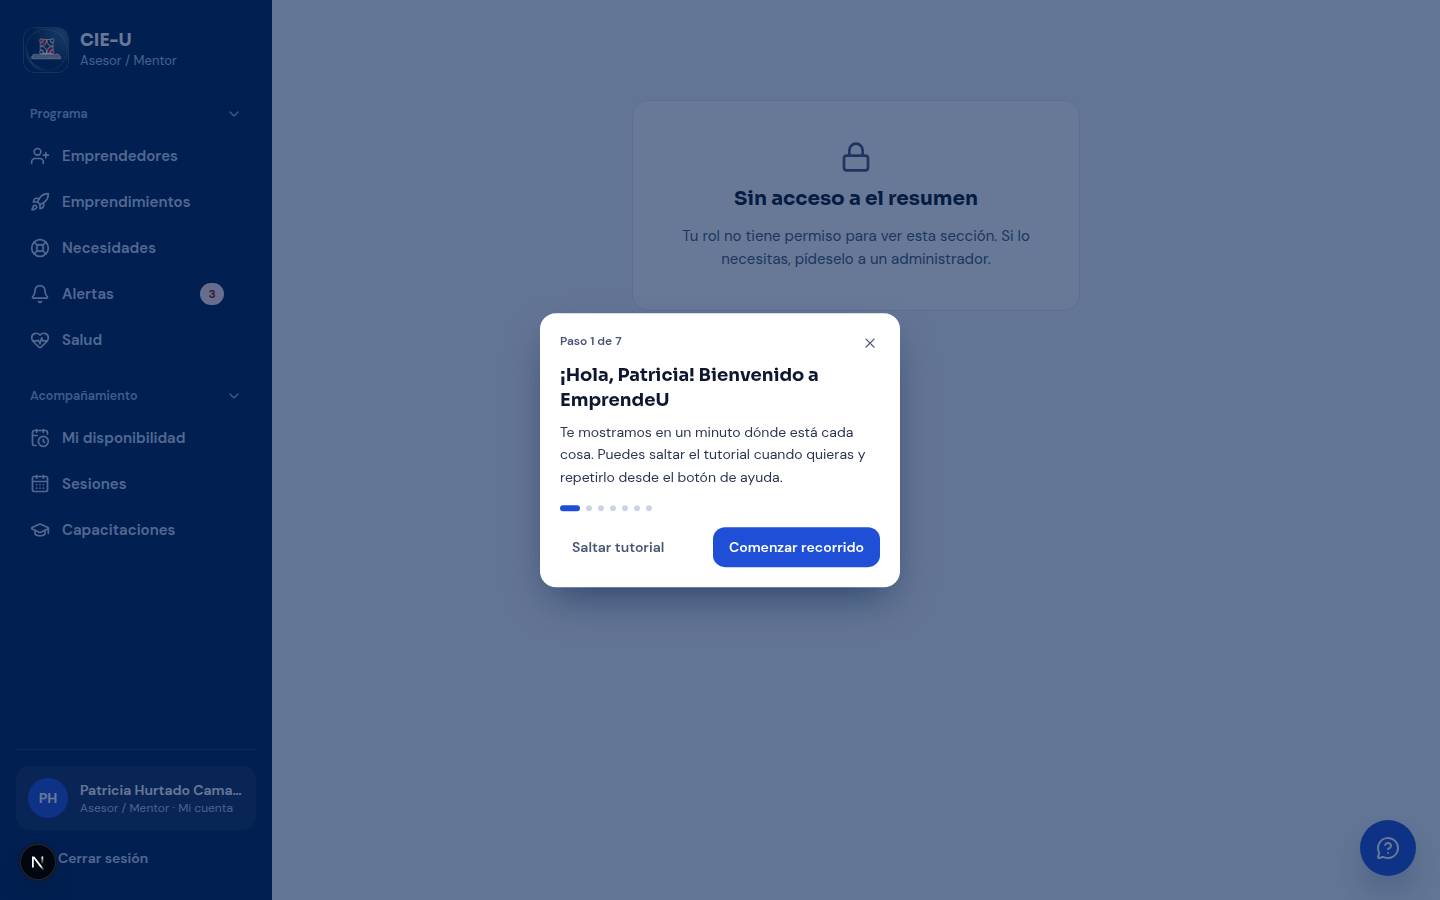
\includegraphics[width=0.97\textwidth,keepaspectratio]{imagenes/web_tutorial_inicio.png}}
\par\vspace{3pt}\begin{flushleft}\small \textit{Nota.} El tutorial se adapta al rol de quien ingresa.\end{flushleft}
\end{figure}

\textbf{Asistente de ayuda.} El botón circular de la esquina inferior derecha abre el «Asistente de ayuda». Se puede escribir una pregunta («¿Cómo registro una sesión?») o elegir una sugerencia. Cuando la IA no está disponible responde con una guía rápida y lo indica: «Respuesta de la guía rápida (IA no disponible ahora).».

\begin{figure}[H]\singlespacing
\caption{Asistente de ayuda}\label{fig:web_chat_ayuda}
\centering\fbox{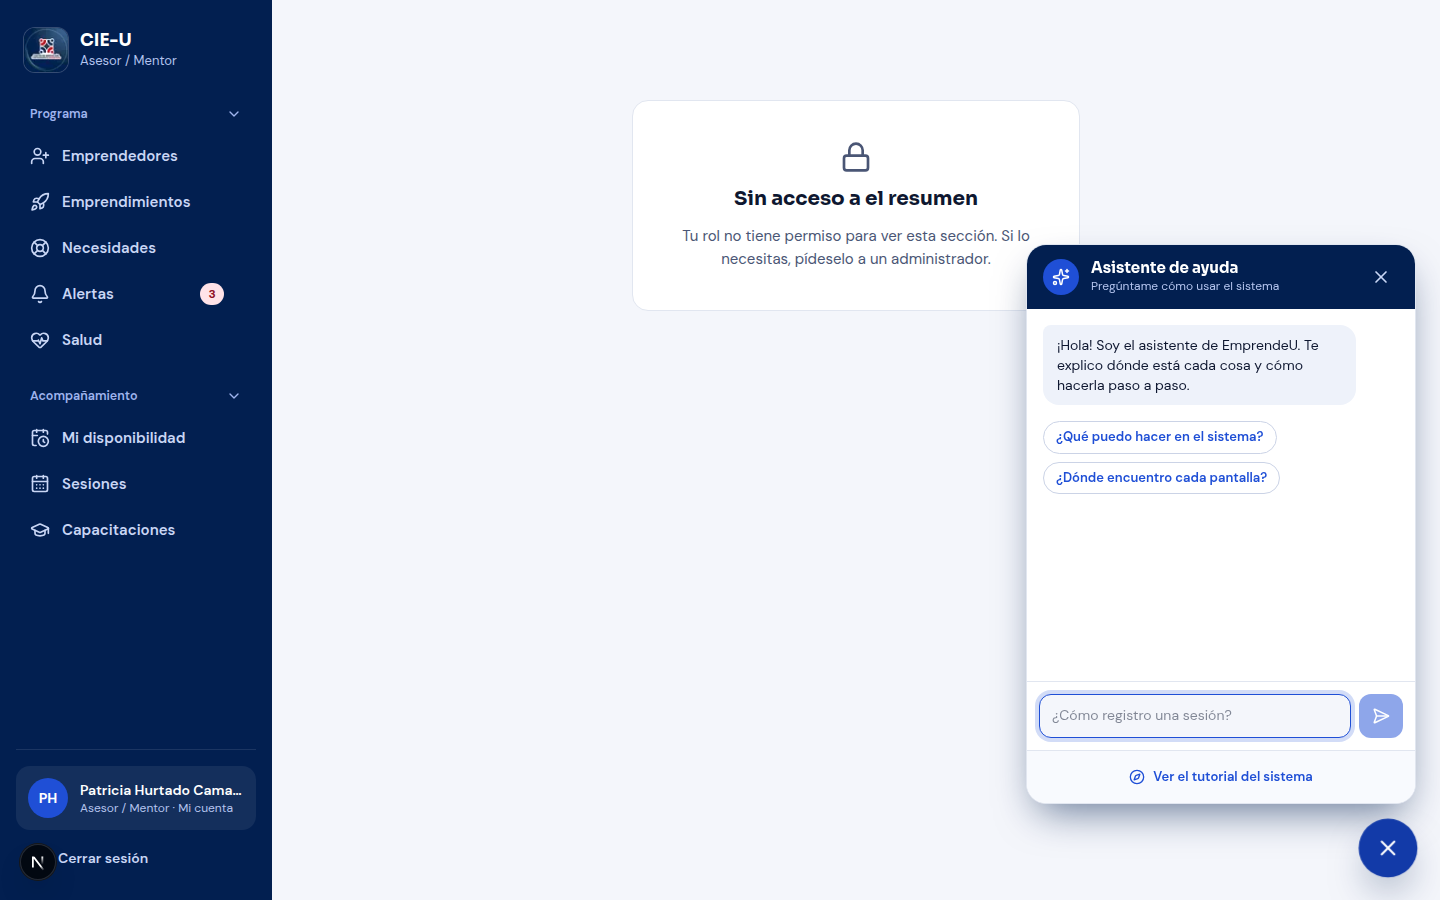
\includegraphics[width=0.97\textwidth,keepaspectratio]{imagenes/web_chat_ayuda.png}}
\par\vspace{3pt}\begin{flushleft}\small \textit{Nota.} Las sugerencias cambian según la pantalla.\end{flushleft}
\end{figure}

\subsection*{5.6. Aplicación móvil}

\addcontentsline{toc}{subsection}{5.6. Aplicación móvil}

\subsubsection*{5.6.1. Inicio}

\addcontentsline{toc}{subsubsection}{5.6.1. Inicio}

\textbf{Roles:} emprendedor. Muestra el saludo, el estado de conexión («En línea» o «Sin conexión»), la campana de notificaciones, el nivel y el XP, la etapa, el «SIGUIENTE RETO», los «Compromisos pendientes» y «Mis avances». Si no hay emprendimiento registrado, aparece «Registra tu emprendimiento».

\begin{enumerate}
\item \textbf{Registrar el emprendimiento:} escribir «Nombre del emprendimiento» y tocar «Registrar emprendimiento».
\item \textbf{Marcar un compromiso:} tocar la casilla del compromiso. Funciona también sin conexión y queda «Pendiente de sincronizar».
\item \textbf{Registrar un avance:} tocar «Registrar avance», describir lo logrado en «¿Qué avanzaste?» y tocar «Guardar».
\end{enumerate}

\begin{figure}[H]\singlespacing
\caption{Pantalla Inicio de la aplicación}\label{fig:movil_inicio}
\centering\fbox{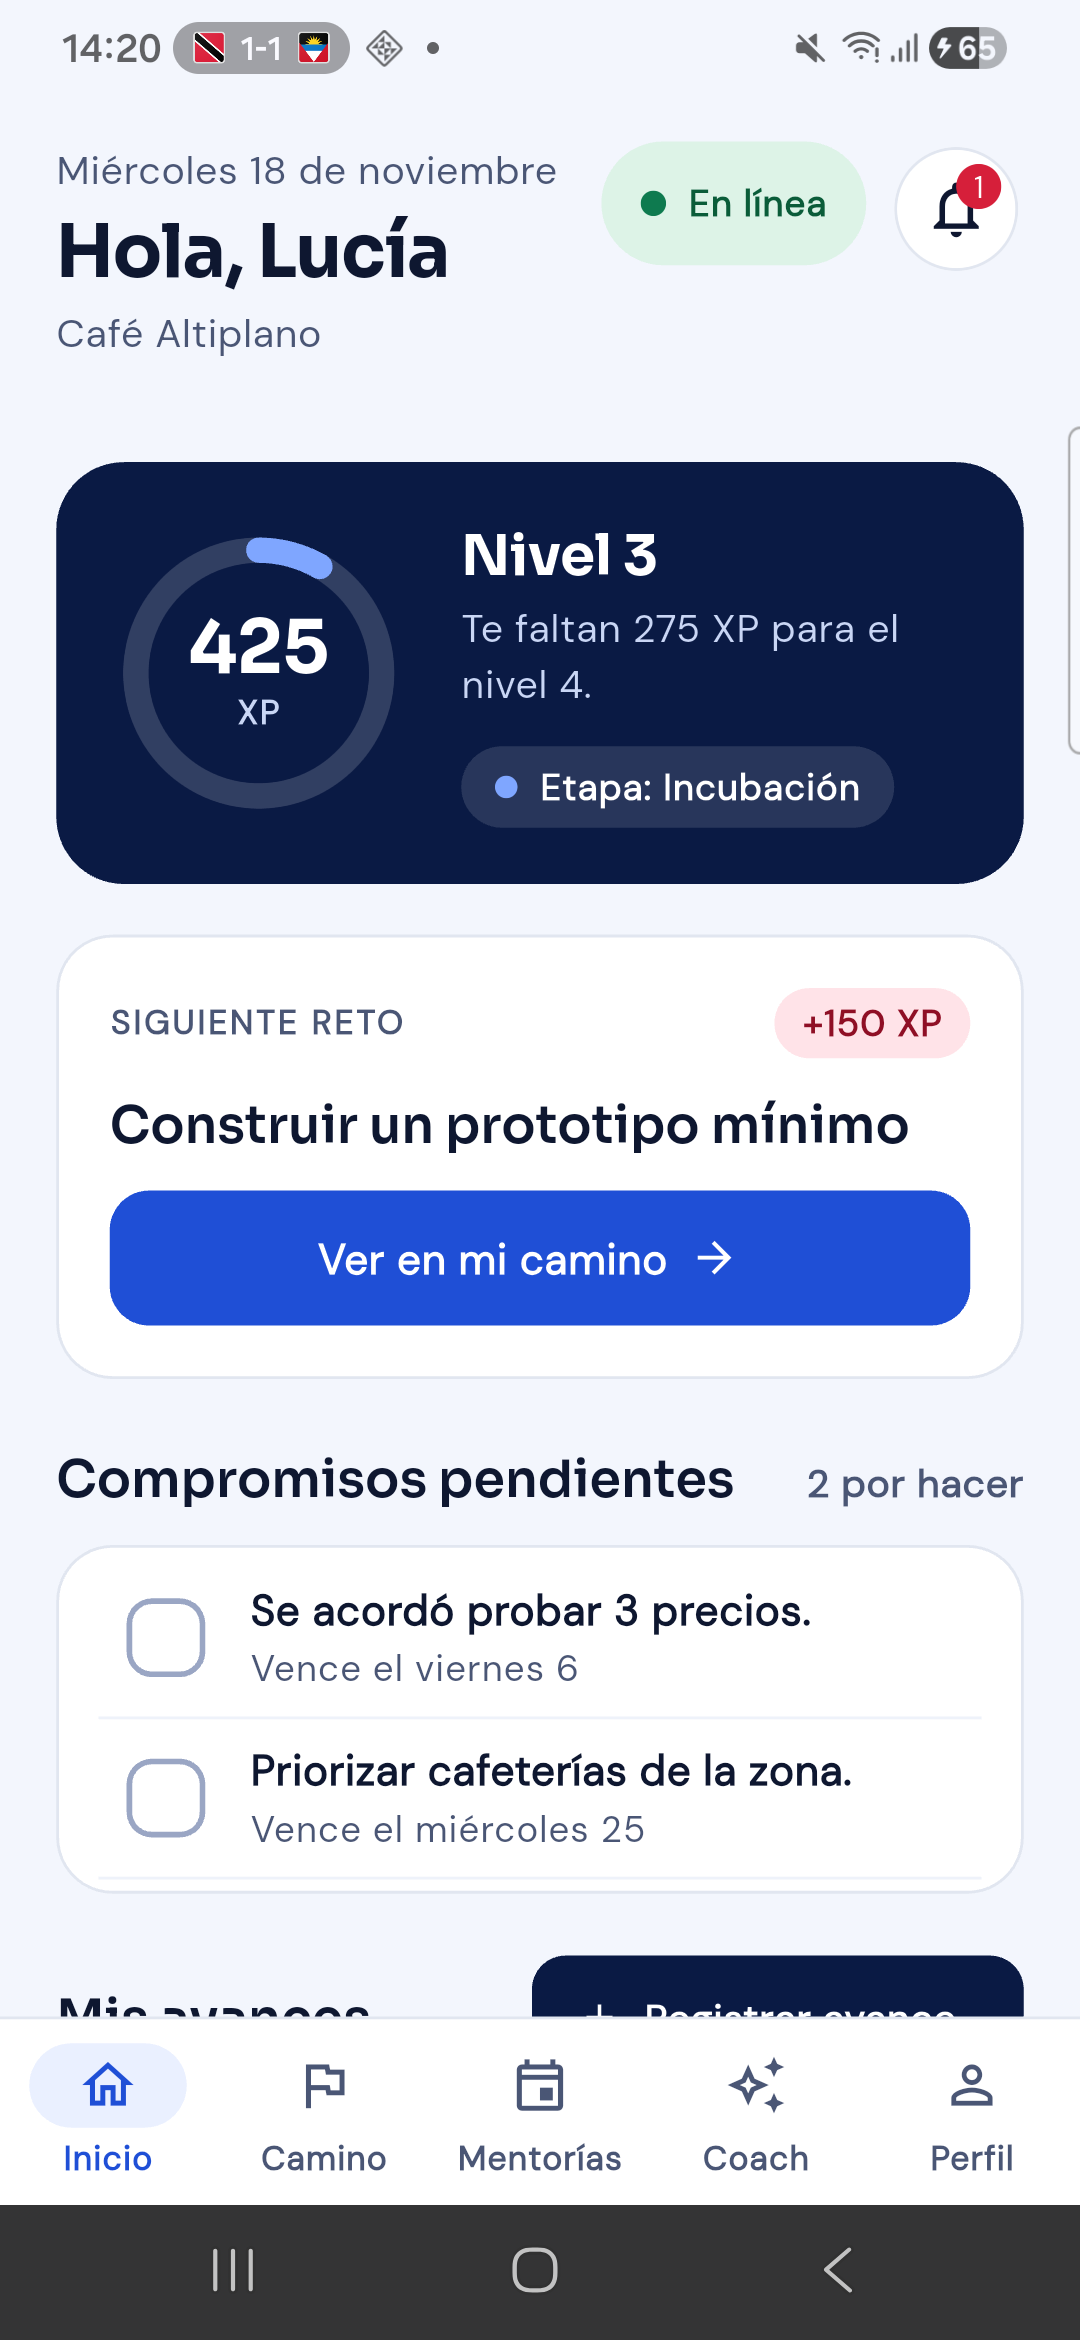
\includegraphics[height=0.52\textheight,keepaspectratio]{imagenes/movil_inicio.png}}
\par\vspace{3pt}\begin{flushleft}\small \textit{Nota.} Resumen del progreso del emprendimiento.\end{flushleft}
\end{figure}

\subsubsection*{5.6.2. Camino}

\addcontentsline{toc}{subsubsection}{5.6.2. Camino}

Muestra el mapa de retos del emprendimiento por etapa, con estados Cumplido, En curso y Bloqueado, y los puntos de XP.

\begin{enumerate}
\item Abrir «Camino» y tocar un reto.
\item Leer los requisitos. Si es necesario, escribir la «Evidencia» o adjuntar un archivo.
\item Tocar «Marcar como cumplido» (requiere conexión).
\item Aparece una celebración con el XP ganado y, si corresponde, el nuevo nivel o insignia.
\end{enumerate}

\begin{figure}[H]\singlespacing
\caption{Pestaña Camino}\label{fig:movil_camino}
\centering\fbox{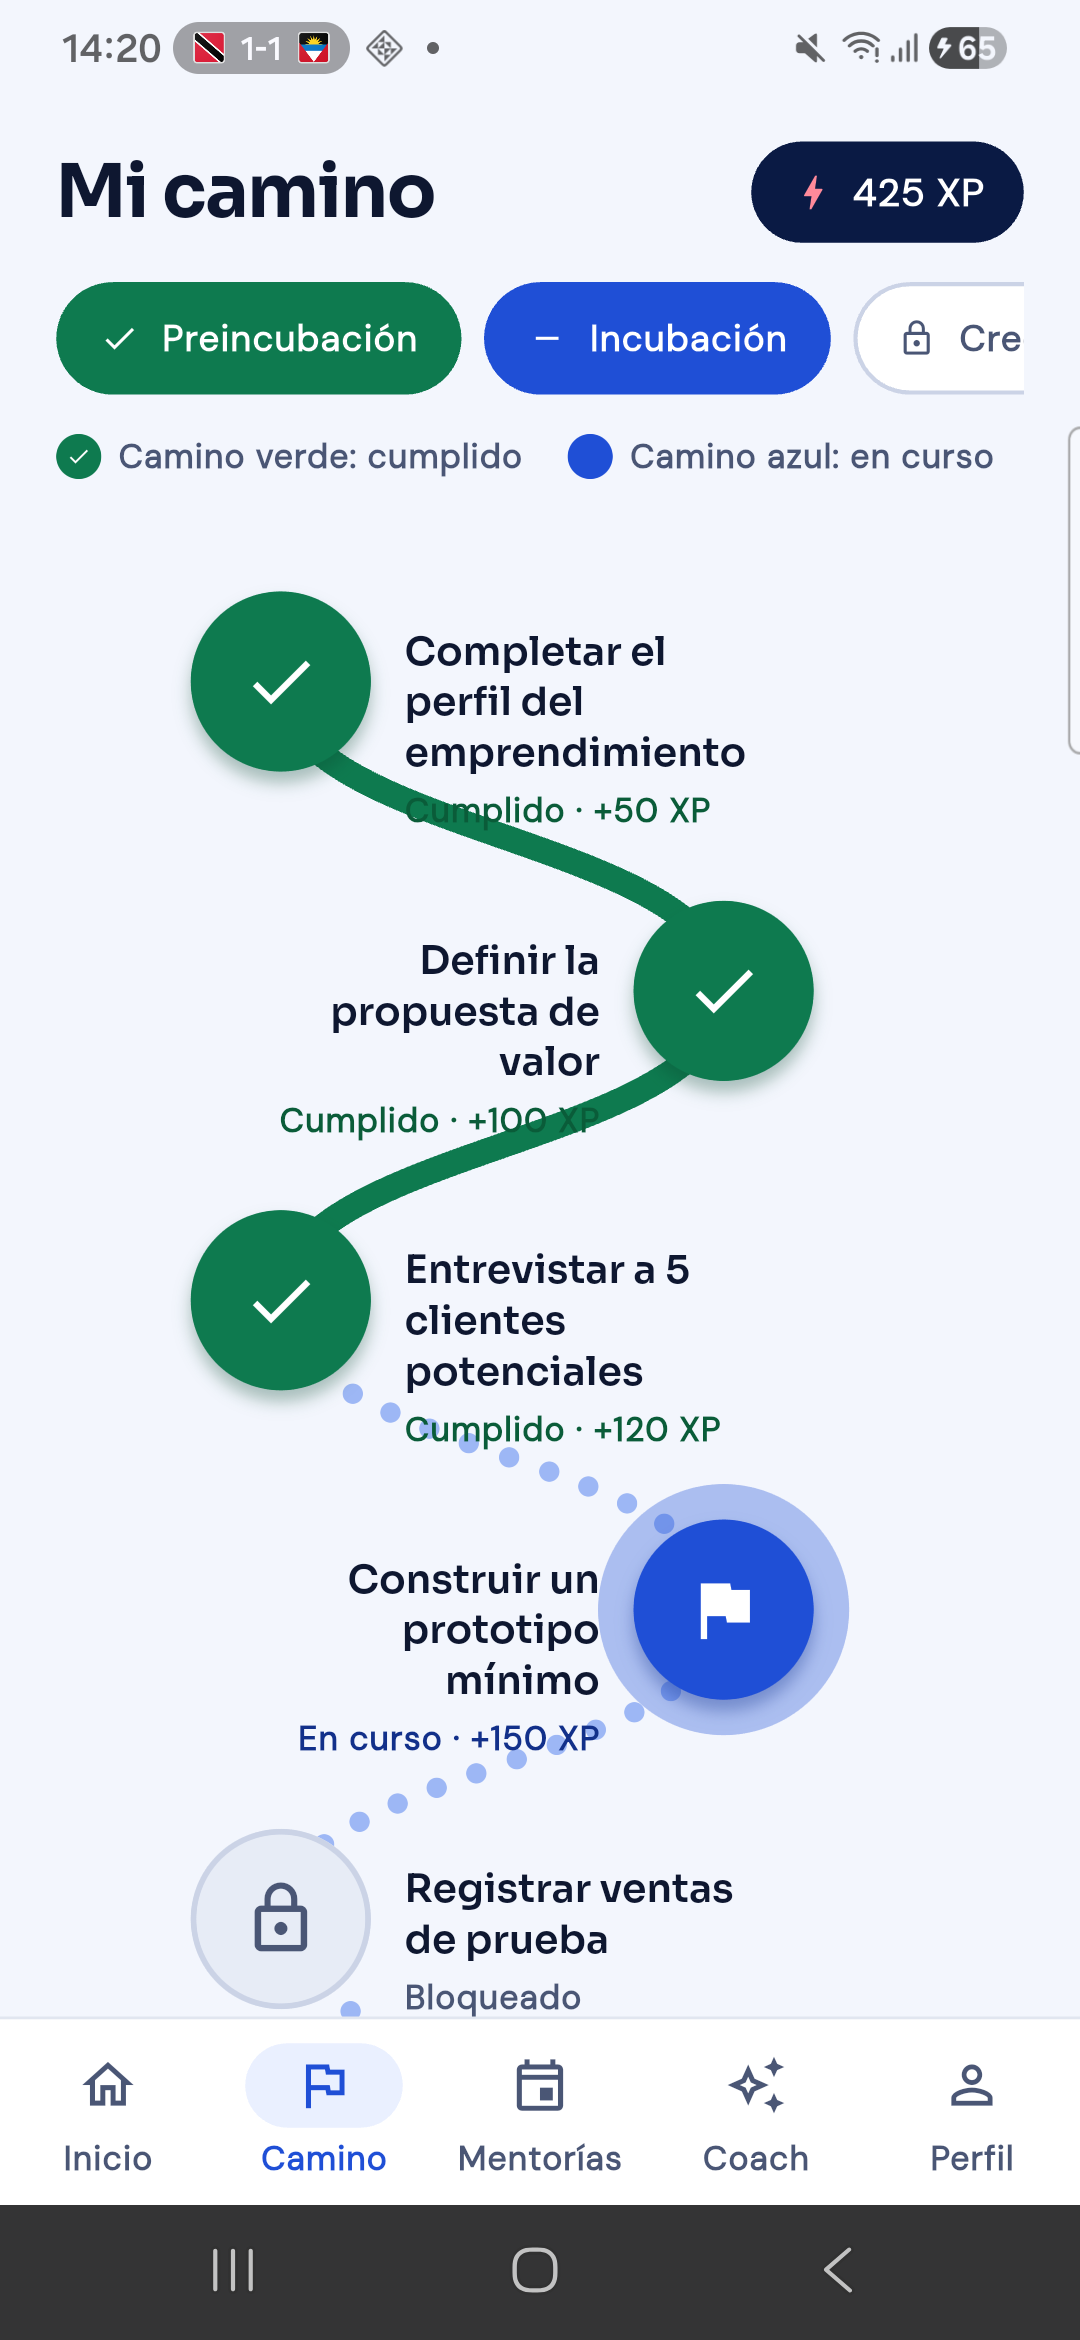
\includegraphics[height=0.52\textheight,keepaspectratio]{imagenes/movil_camino.png}}
\par\vspace{3pt}\begin{flushleft}\small \textit{Nota.} El reto en curso aparece destacado con una bandera.\end{flushleft}
\end{figure}

Un reto bloqueado muestra «Completa el reto anterior para desbloquearlo.». El detalle de XP e insignias está en «Ver experiencia e insignias» del Perfil.

\subsubsection*{5.6.3. Mentorías}

\addcontentsline{toc}{subsubsection}{5.6.3. Mentorías}

\begin{enumerate}
\item Abrir «Mentorías». Las pestañas «Próximas», «Realizadas» y «Canceladas» filtran la lista; «Filtrar por periodo» acota las fechas.
\item \textbf{Agendar:} «Agendar mentoría» $\rightarrow$ elegir asesor $\rightarrow$ elegir el día (14 días) $\rightarrow$ elegir el horario $\rightarrow$ opcionalmente escribir el «Tema» $\rightarrow$ «Confirmar mentoría».
\item \textbf{Cancelar:} abrir una mentoría programada y tocar «Cancelar mentoría», confirmando el diálogo.
\item \textbf{Historial:} «Ver historial del emprendimiento».
\item \textbf{Tareas:} «Tareas y compromisos», con los filtros Pendientes, Cumplidas, Compromisos e Hitos.
\end{enumerate}

\begin{figure}[H]\singlespacing
\caption{Pestaña Mentorías}\label{fig:movil_mentorias}
\centering\fbox{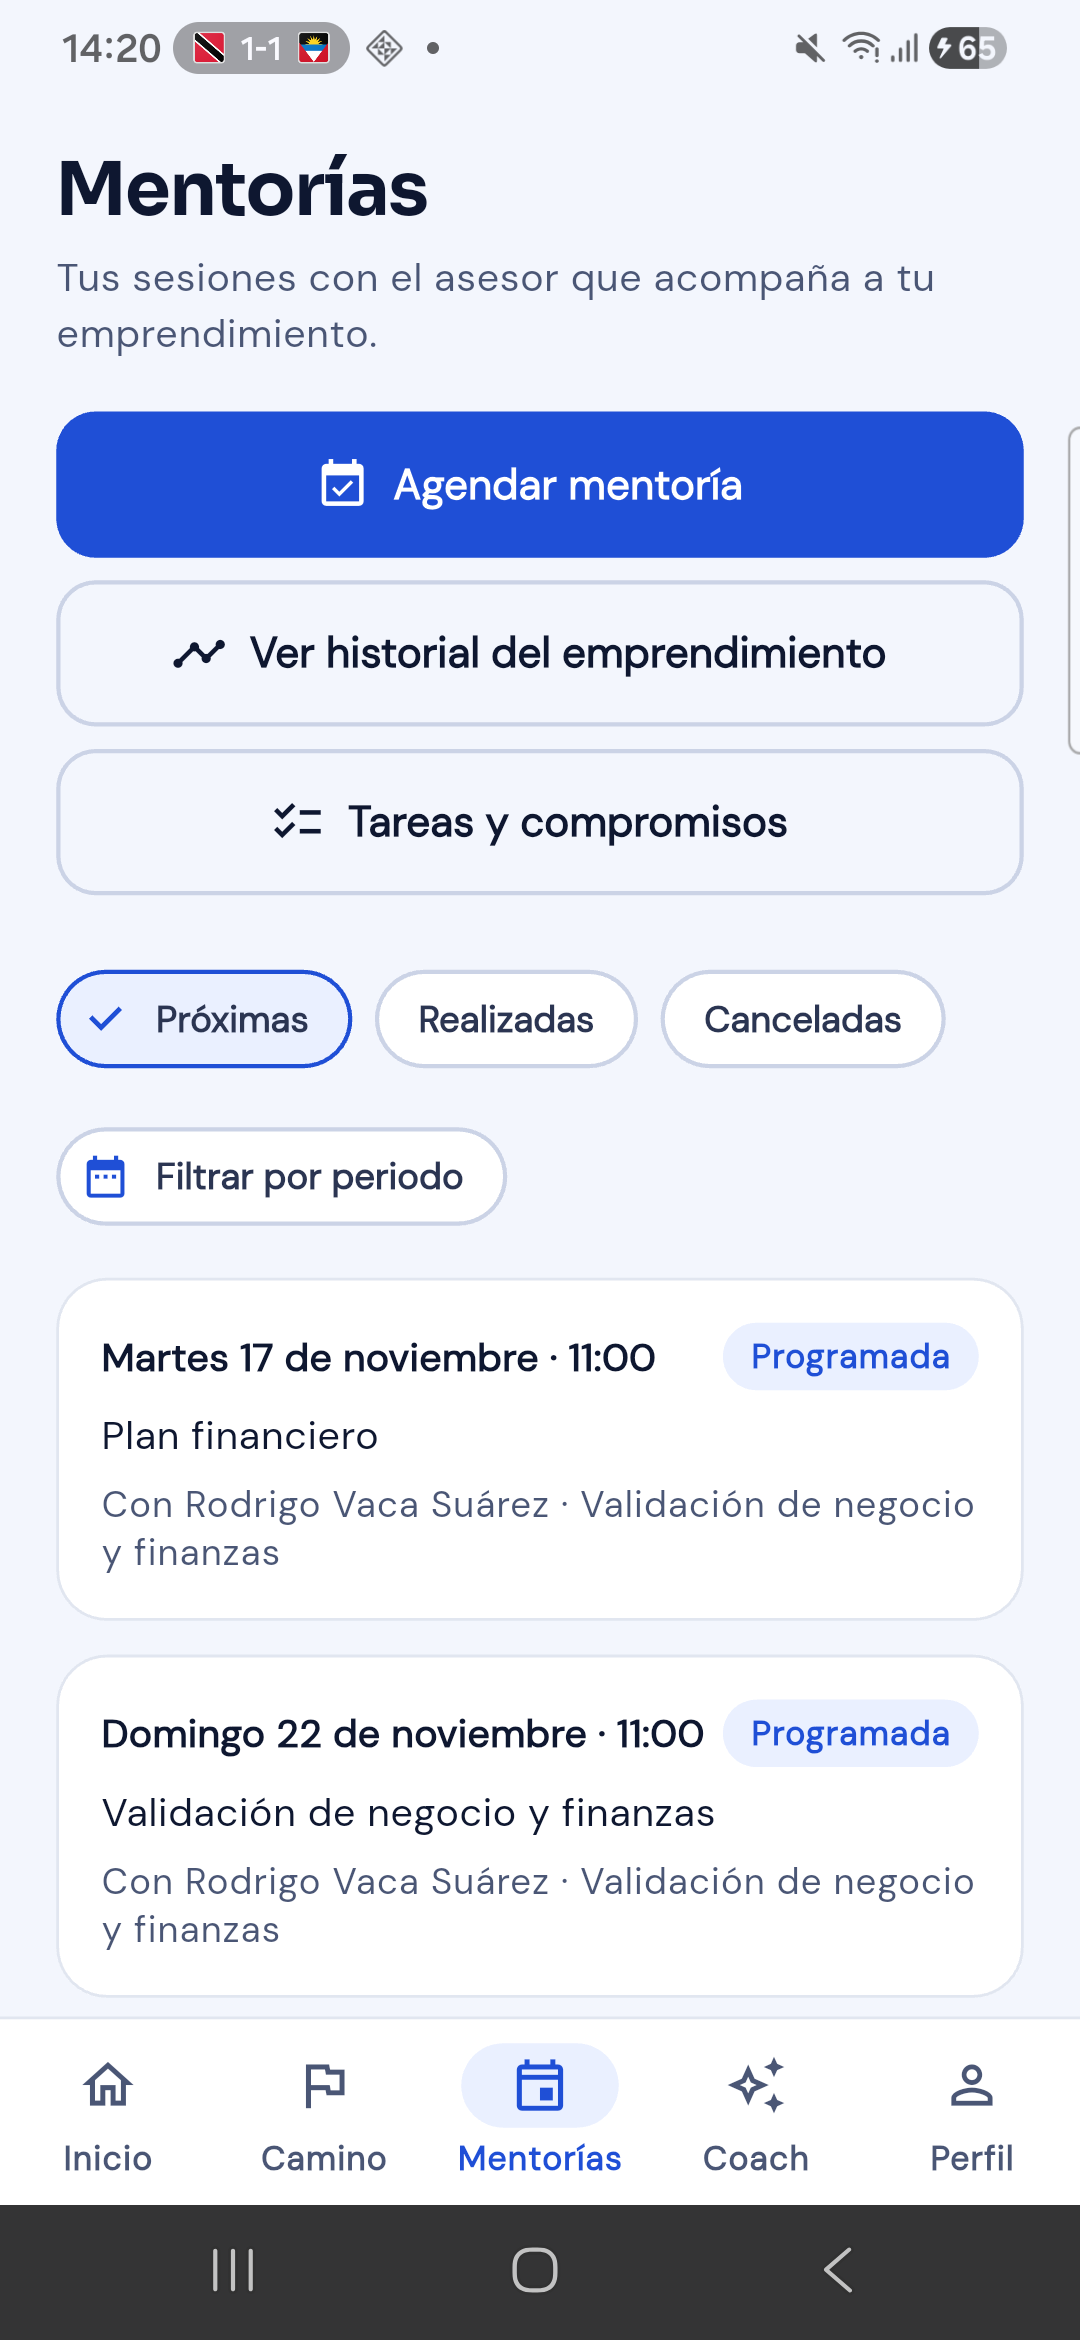
\includegraphics[height=0.52\textheight,keepaspectratio]{imagenes/movil_mentorias.png}}
\par\vspace{3pt}\begin{flushleft}\small \textit{Nota.} Las mentorías próximas aparecen con estado «Programada».\end{flushleft}
\end{figure}

\begin{figure}[H]\singlespacing
\caption{Agendar una mentoría}\label{fig:movil_agendar}
\centering\fbox{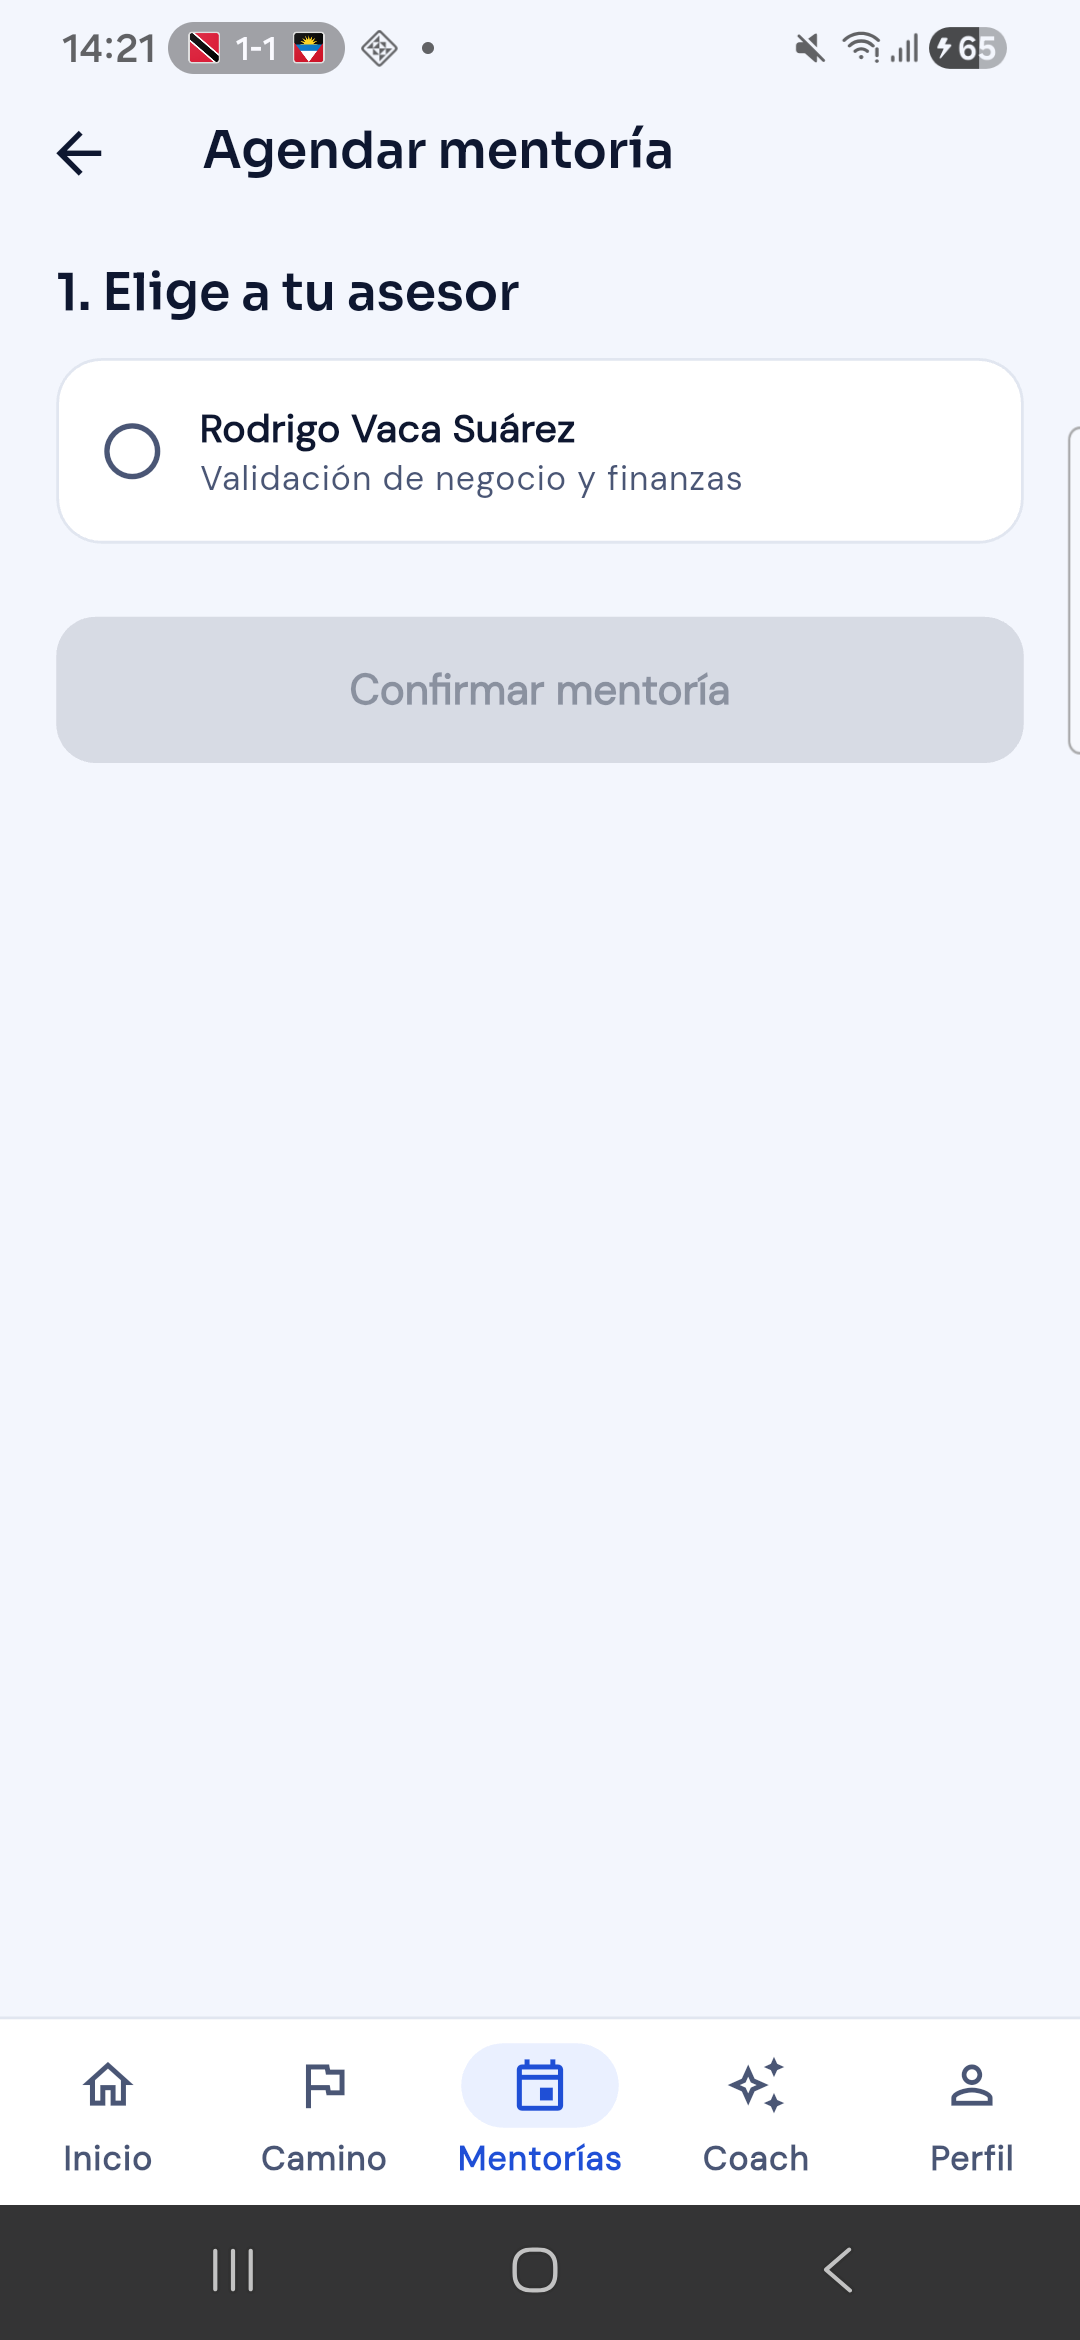
\includegraphics[height=0.52\textheight,keepaspectratio]{imagenes/movil_agendar.png}}
\par\vspace{3pt}\begin{flushleft}\small \textit{Nota.} Solo se puede agendar con asesores asignados.\end{flushleft}
\end{figure}

\begin{figure}[H]\singlespacing
\caption{Historial del emprendimiento}\label{fig:movil_historial}
\centering\fbox{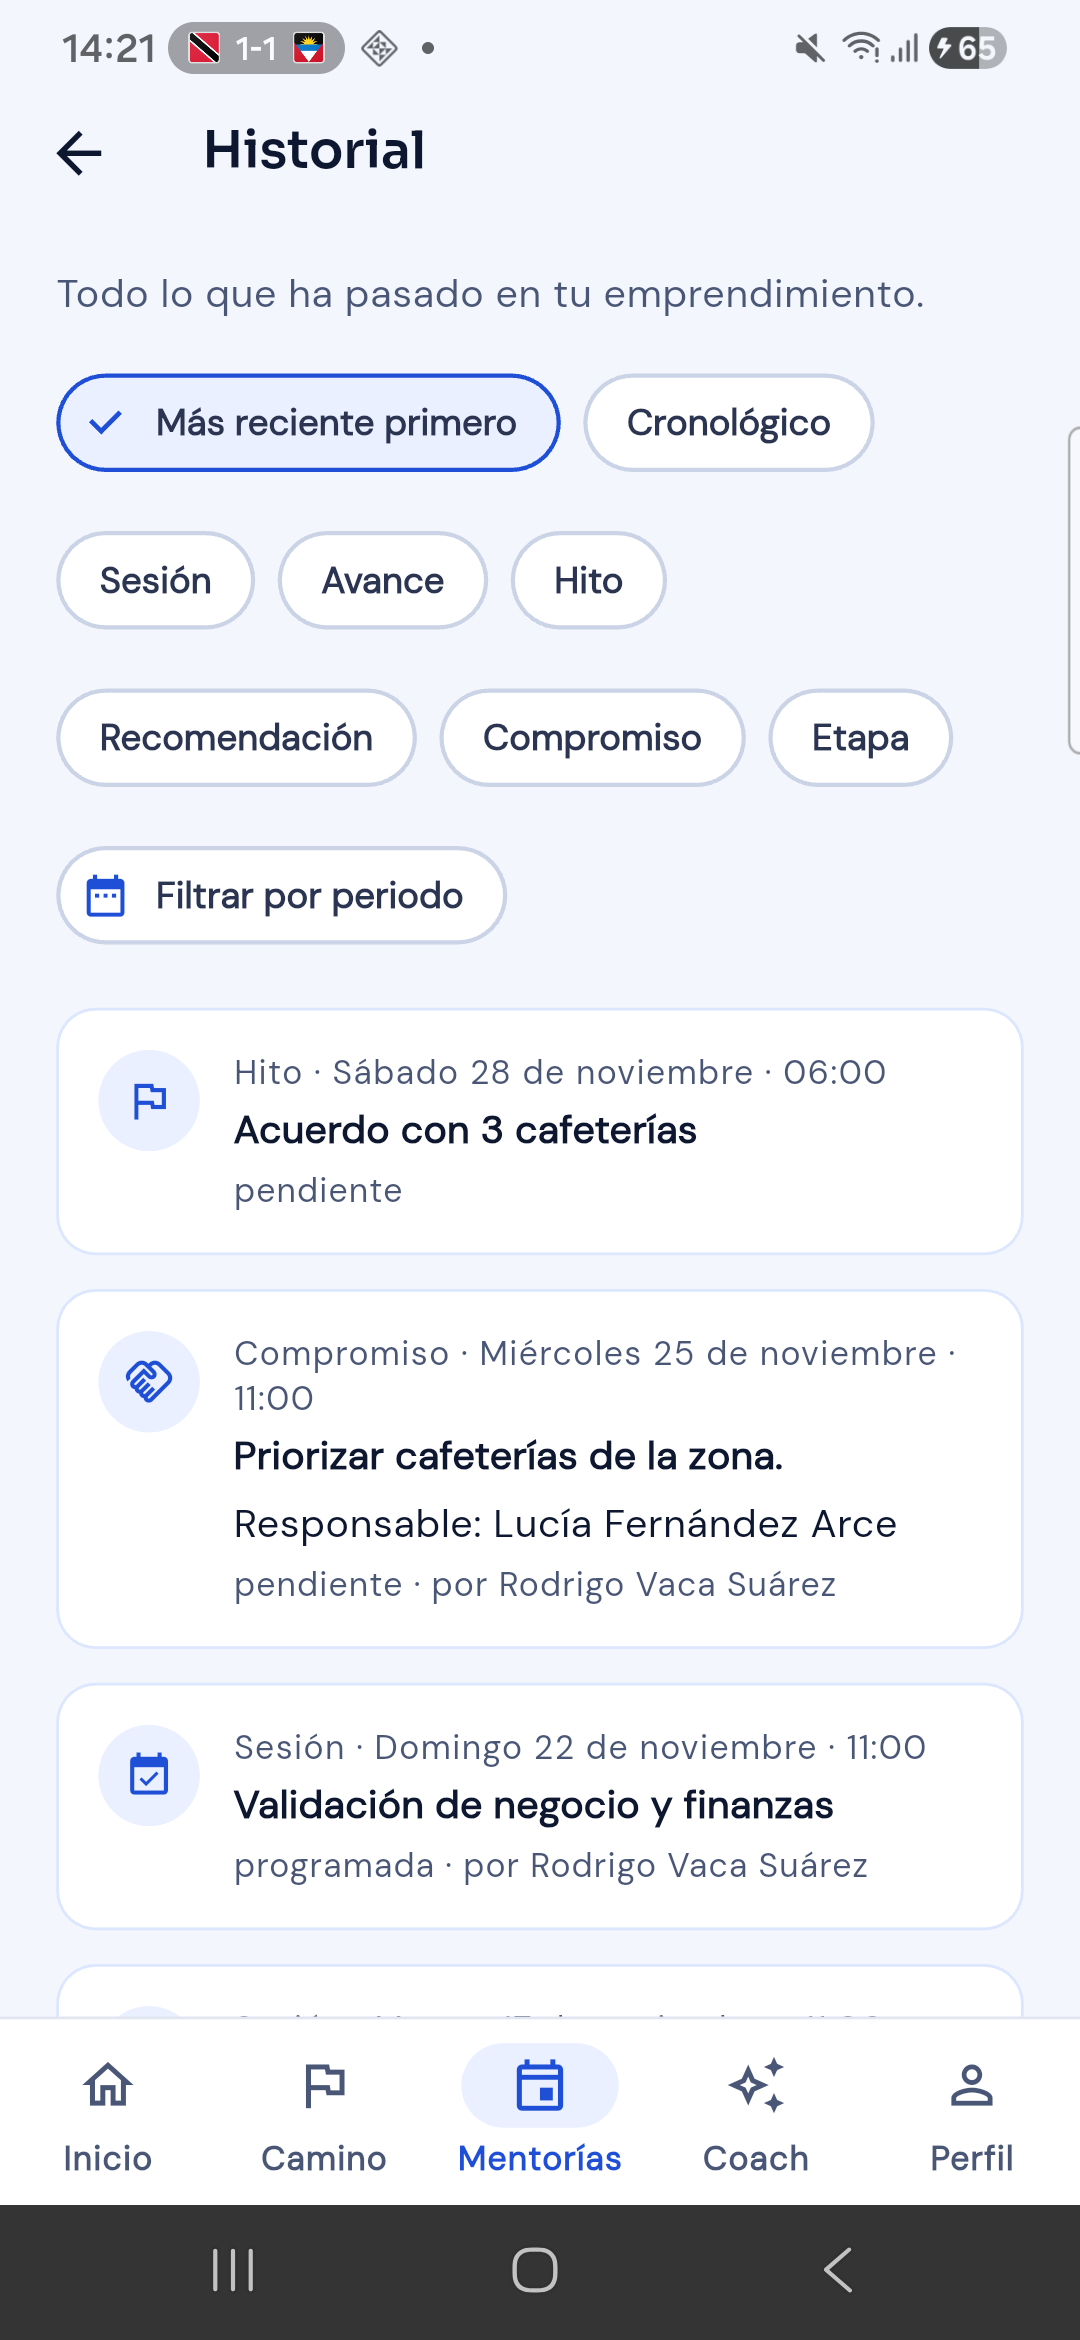
\includegraphics[height=0.52\textheight,keepaspectratio]{imagenes/movil_historial.png}}
\par\vspace{3pt}\begin{flushleft}\small \textit{Nota.} Se puede ordenar y filtrar por tipo de evento.\end{flushleft}
\end{figure}

\begin{figure}[H]\singlespacing
\caption{Tareas y compromisos}\label{fig:movil_tareas}
\centering\fbox{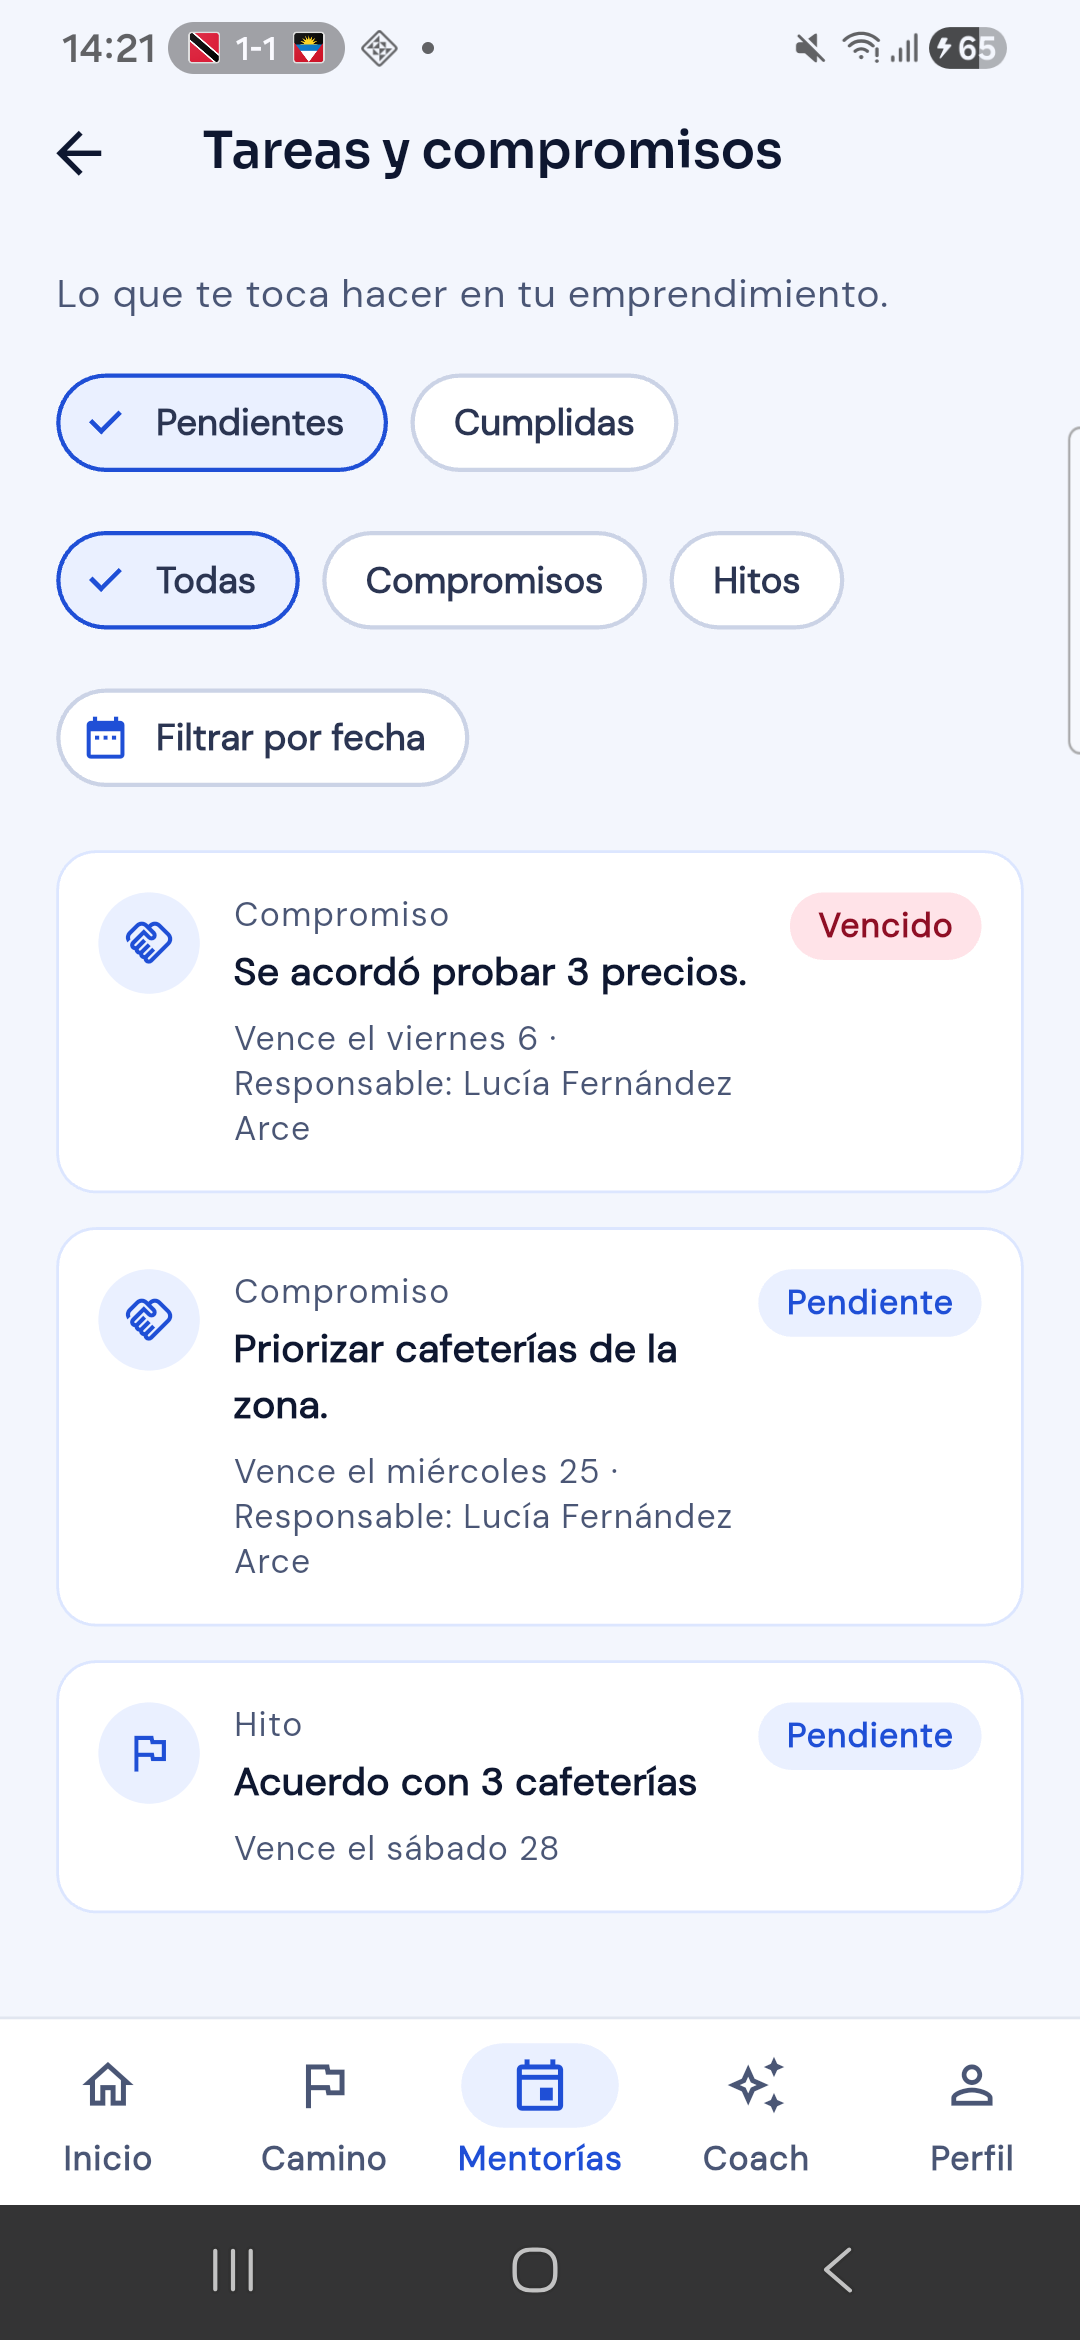
\includegraphics[height=0.52\textheight,keepaspectratio]{imagenes/movil_tareas.png}}
\par\vspace{3pt}\begin{flushleft}\small \textit{Nota.} Los compromisos vencidos se marcan en rojo.\end{flushleft}
\end{figure}

Si no hay asesor asignado: «Todavía no tienes un asesor asignado. El CIE-U te asignará uno cuando tu emprendimiento esté listo.». Si el horario se ocupó: «Ese horario ya no está disponible. Elige otro.».

\subsubsection*{5.6.4. Coach IA}

\addcontentsline{toc}{subsubsection}{5.6.4. Coach IA}

\begin{enumerate}
\item Abrir «Coach».
\item Escribir la consulta en «Escribe tu pregunta» o tocar una sugerencia, y tocar «Enviar».
\item La respuesta cita sus «Fuentes». Si no hay información suficiente o el tema es legal o financiero, se ofrece «Agendar una mentoría».
\item «Conversaciones anteriores» muestra el historial y «Nueva conversación» inicia otra.
\item Con la IA instalada, los chips «En tu celular» y «En línea» permiten elegir el modo. «Tus archivos» permite añadir PDF, Word, TXT o MD (hasta 20 MB) que se analizan solo en el teléfono.
\end{enumerate}

\begin{figure}[H]\singlespacing
\caption{Pestaña Coach IA}\label{fig:movil_coach}
\centering\fbox{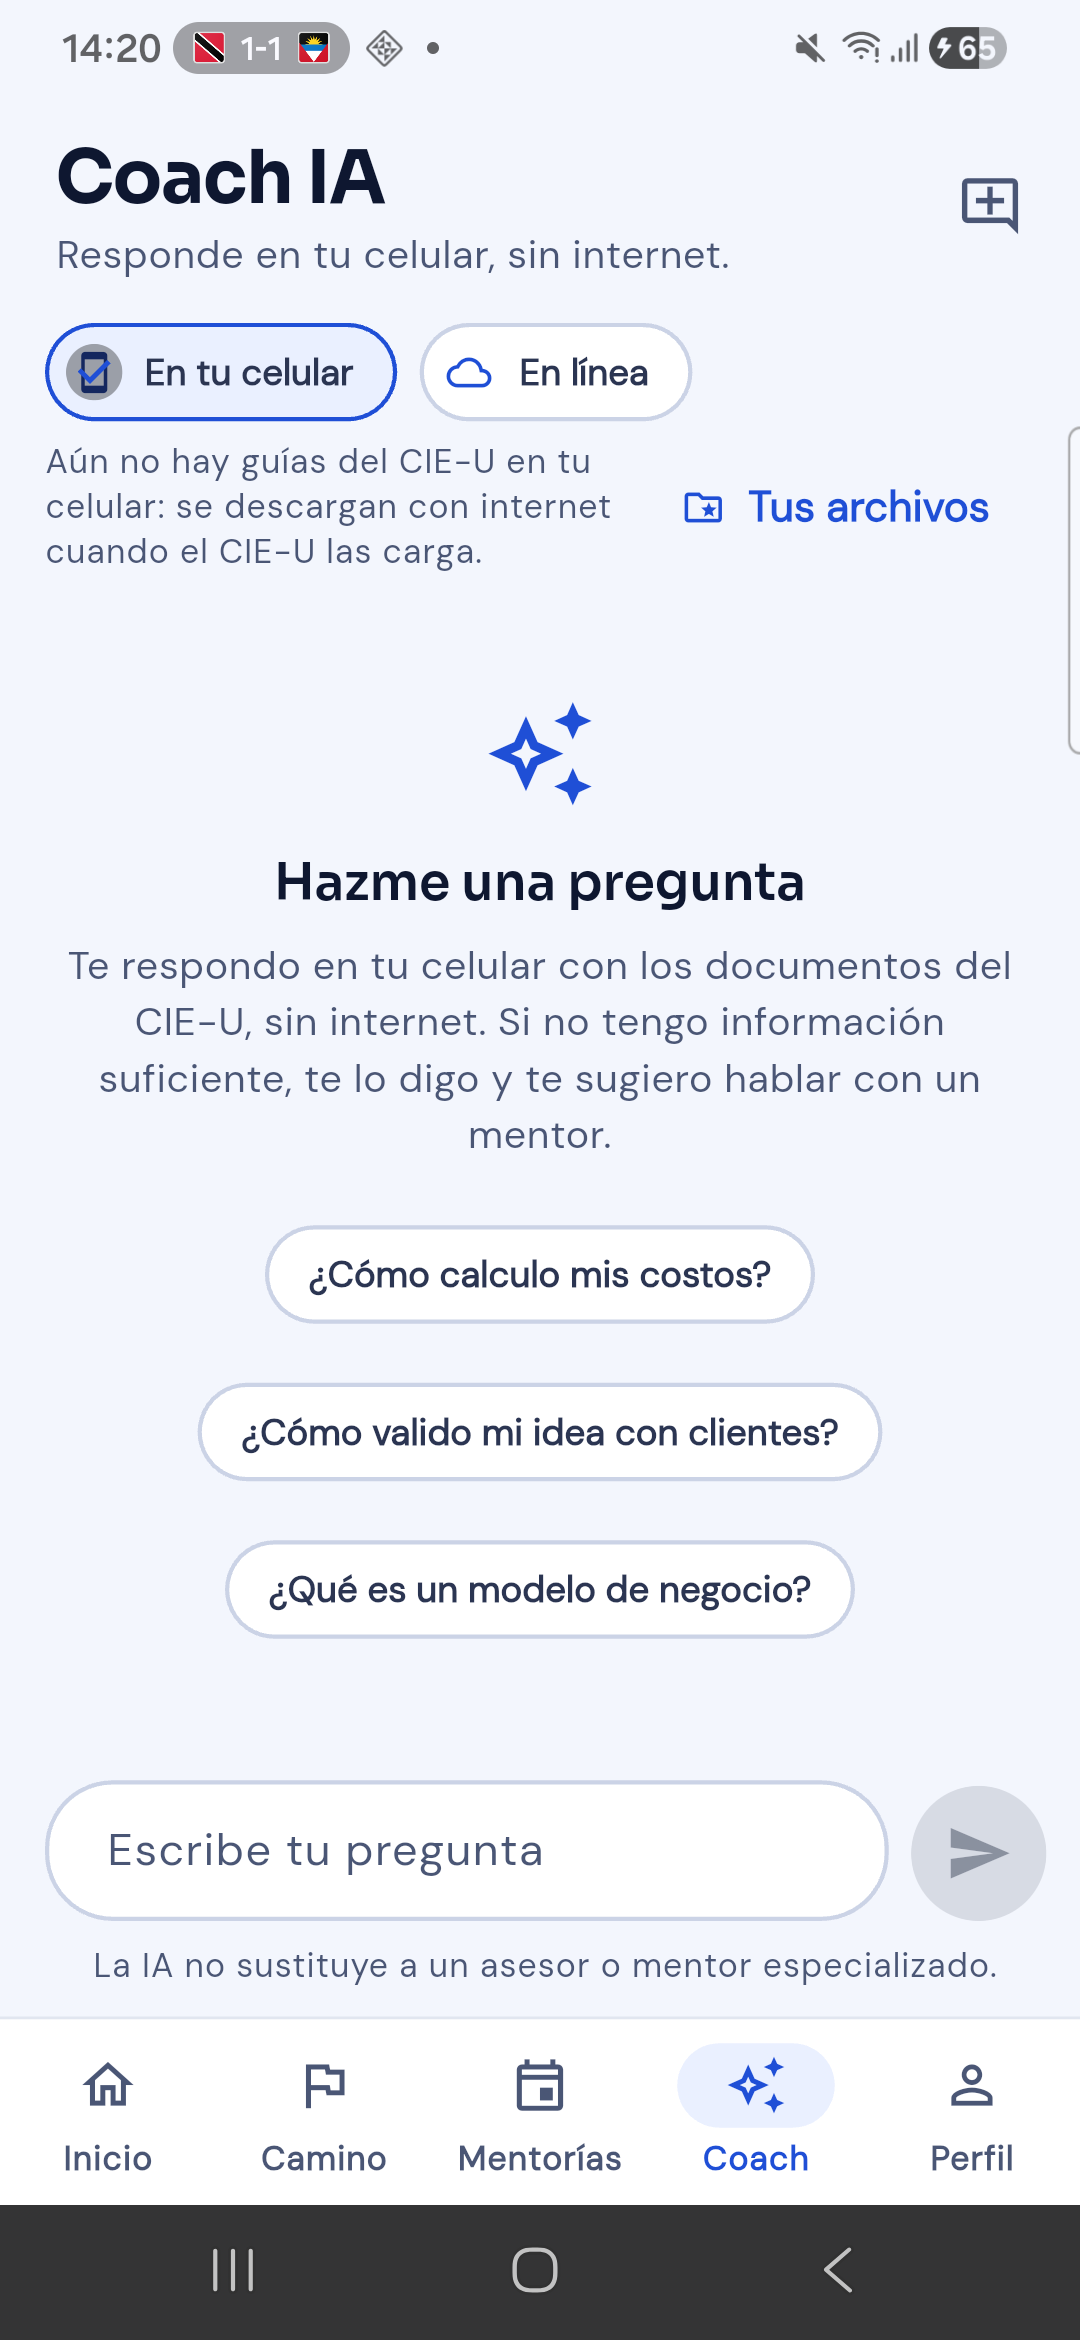
\includegraphics[height=0.52\textheight,keepaspectratio]{imagenes/movil_coach.png}}
\par\vspace{3pt}\begin{flushleft}\small \textit{Nota.} Pantalla del modo «En tu celular».\end{flushleft}
\end{figure}

El coach muestra siempre el aviso «La IA no sustituye a un asesor o mentor especializado.». Longitud máxima del mensaje: 2000 caracteres.

\subsubsection*{5.6.5. Perfil}

\addcontentsline{toc}{subsubsection}{5.6.5. Perfil}

Reúne los datos de la persona, «Mi emprendimiento», el XP, las insignias y los accesos a otras funciones.

\begin{figure}[H]\singlespacing
\caption{Pestaña Perfil}\label{fig:movil_perfil}
\centering\fbox{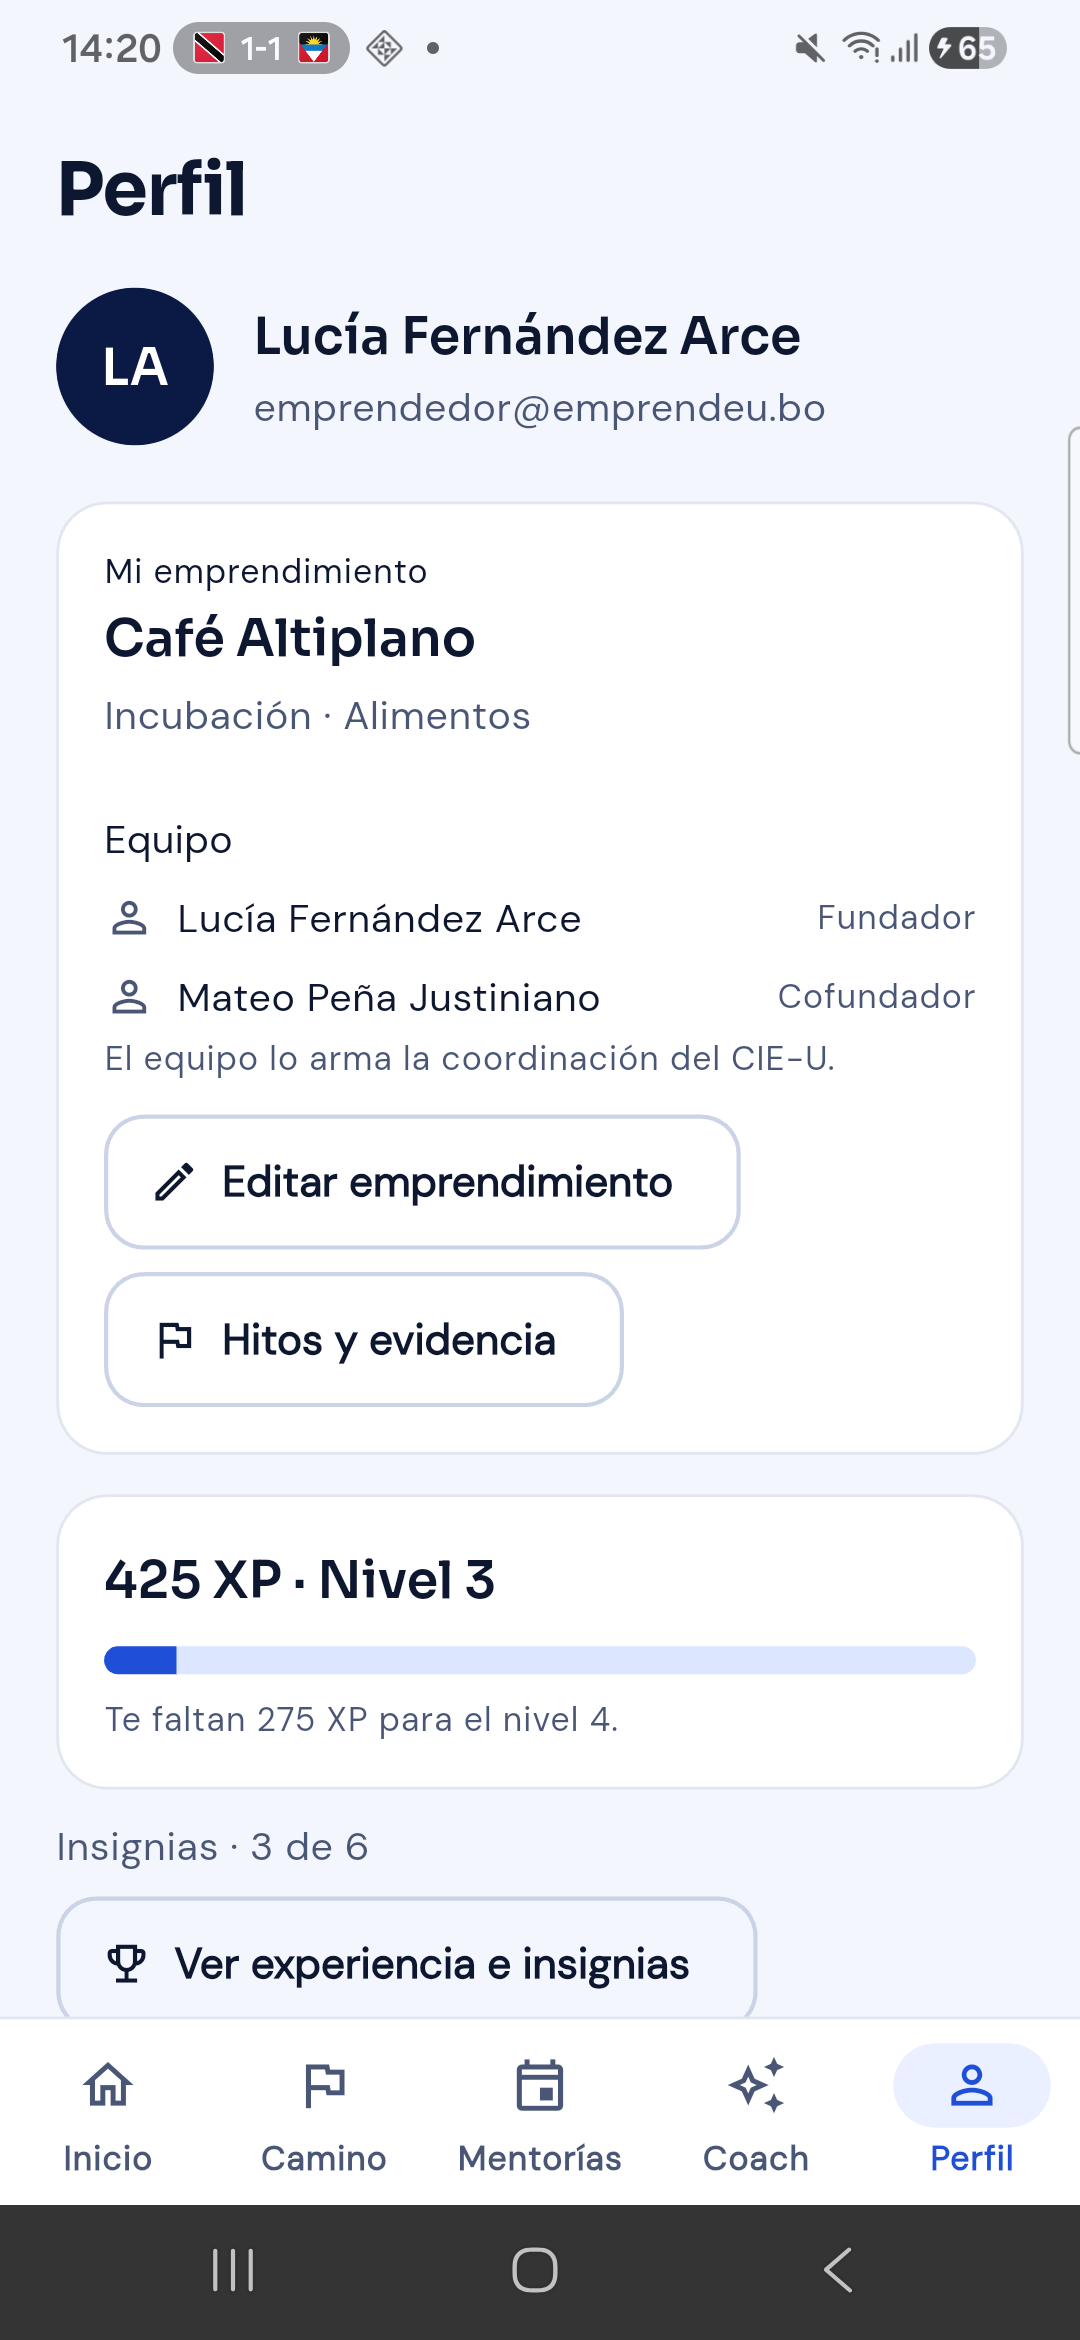
\includegraphics[height=0.52\textheight,keepaspectratio]{imagenes/movil_perfil.png}}
\par\vspace{3pt}\begin{flushleft}\small \textit{Nota.} Incluye el emprendimiento, el equipo y el XP.\end{flushleft}
\end{figure}

\begin{figure}[H]\singlespacing
\caption{Opciones del Perfil}\label{fig:movil_perfil_2}
\centering\fbox{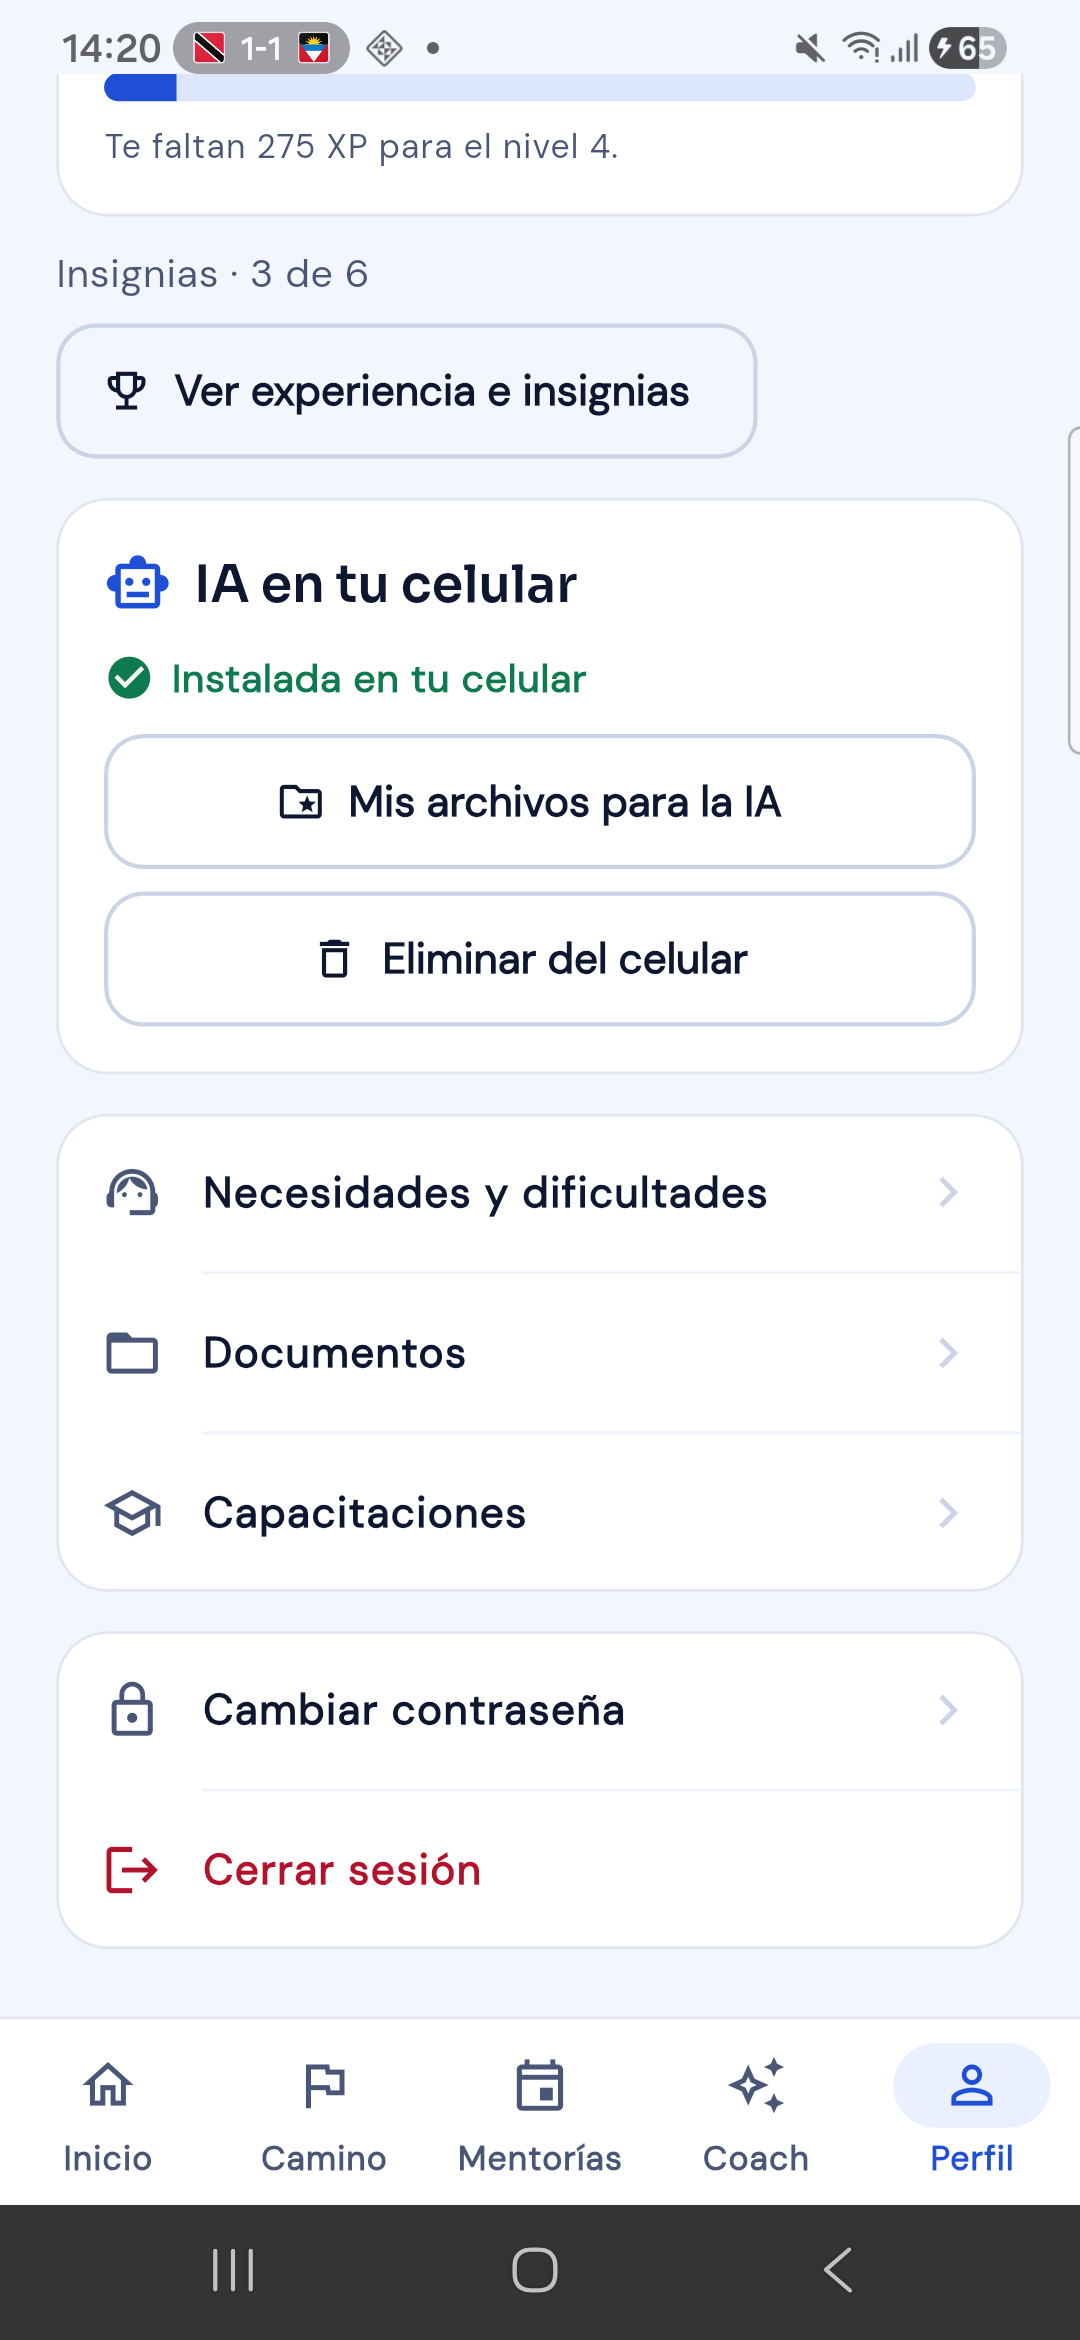
\includegraphics[height=0.52\textheight,keepaspectratio]{imagenes/movil_perfil_2.png}}
\par\vspace{3pt}\begin{flushleft}\small \textit{Nota.} Sección «IA en tu celular» y accesos directos.\end{flushleft}
\end{figure}

\begin{itemize}
\item \textbf{Editar emprendimiento:} cambiar nombre, sector y descripción y tocar «Guardar cambios». La etapa y el estado los define la coordinación.
\item \textbf{Hitos y evidencia:} «Registrar hito» (qué lograste, descripción y evidencia opcional), «Adjuntar evidencia» y «Marcar cumplido».
\item \textbf{IA en tu celular:} «Descargar IA» (confirmar «Descargar»), «Cancelar descarga» y «Eliminar del celular».
\item \textbf{Cambiar contraseña:} contraseña actual, nueva y repetición; se cierran las demás sesiones.
\end{itemize}

\begin{figure}[H]\singlespacing
\caption{Cambiar contraseña}\label{fig:movil_cambiar_password}
\centering\fbox{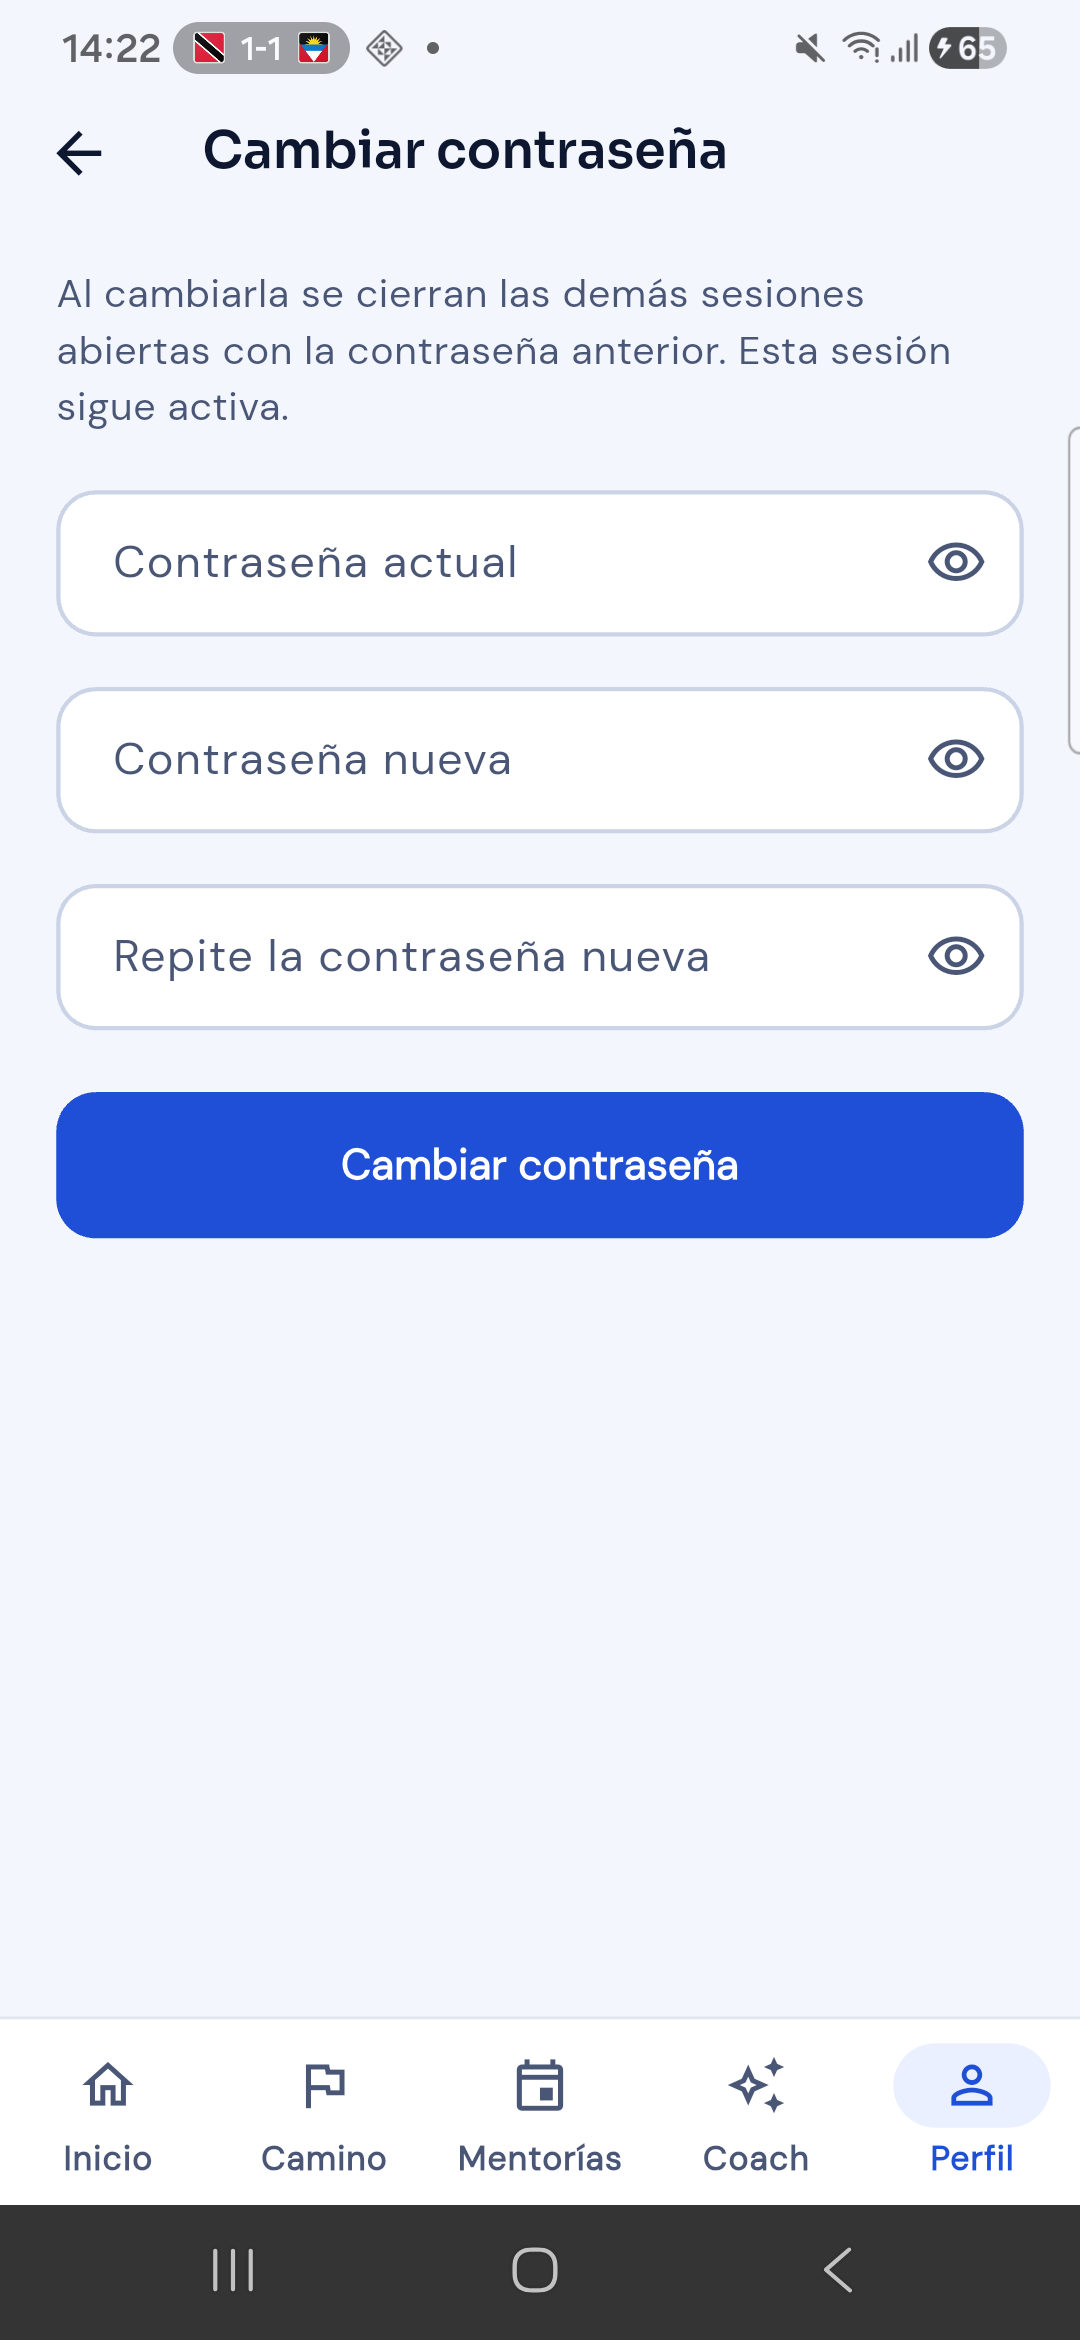
\includegraphics[height=0.52\textheight,keepaspectratio]{imagenes/movil_cambiar_password.png}}
\par\vspace{3pt}\begin{flushleft}\small \textit{Nota.} La sesión actual permanece activa.\end{flushleft}
\end{figure}

\subsubsection*{5.6.6. Necesidades y dificultades}

\addcontentsline{toc}{subsubsection}{5.6.6. Necesidades y dificultades}

\begin{enumerate}
\item Perfil $\rightarrow$ «Necesidades y dificultades» $\rightarrow$ «Reportar».
\item Elegir «Necesidad» o «Dificultad», el «Rubro» y la «Prioridad», y describir el caso en «Descríbelo».
\item Tocar «Enviar reporte». Aparece «Reporte enviado. El CIE-U lo podrá ver.».
\end{enumerate}

\begin{figure}[H]\singlespacing
\caption{Necesidades y dificultades}\label{fig:movil_necesidades}
\centering\fbox{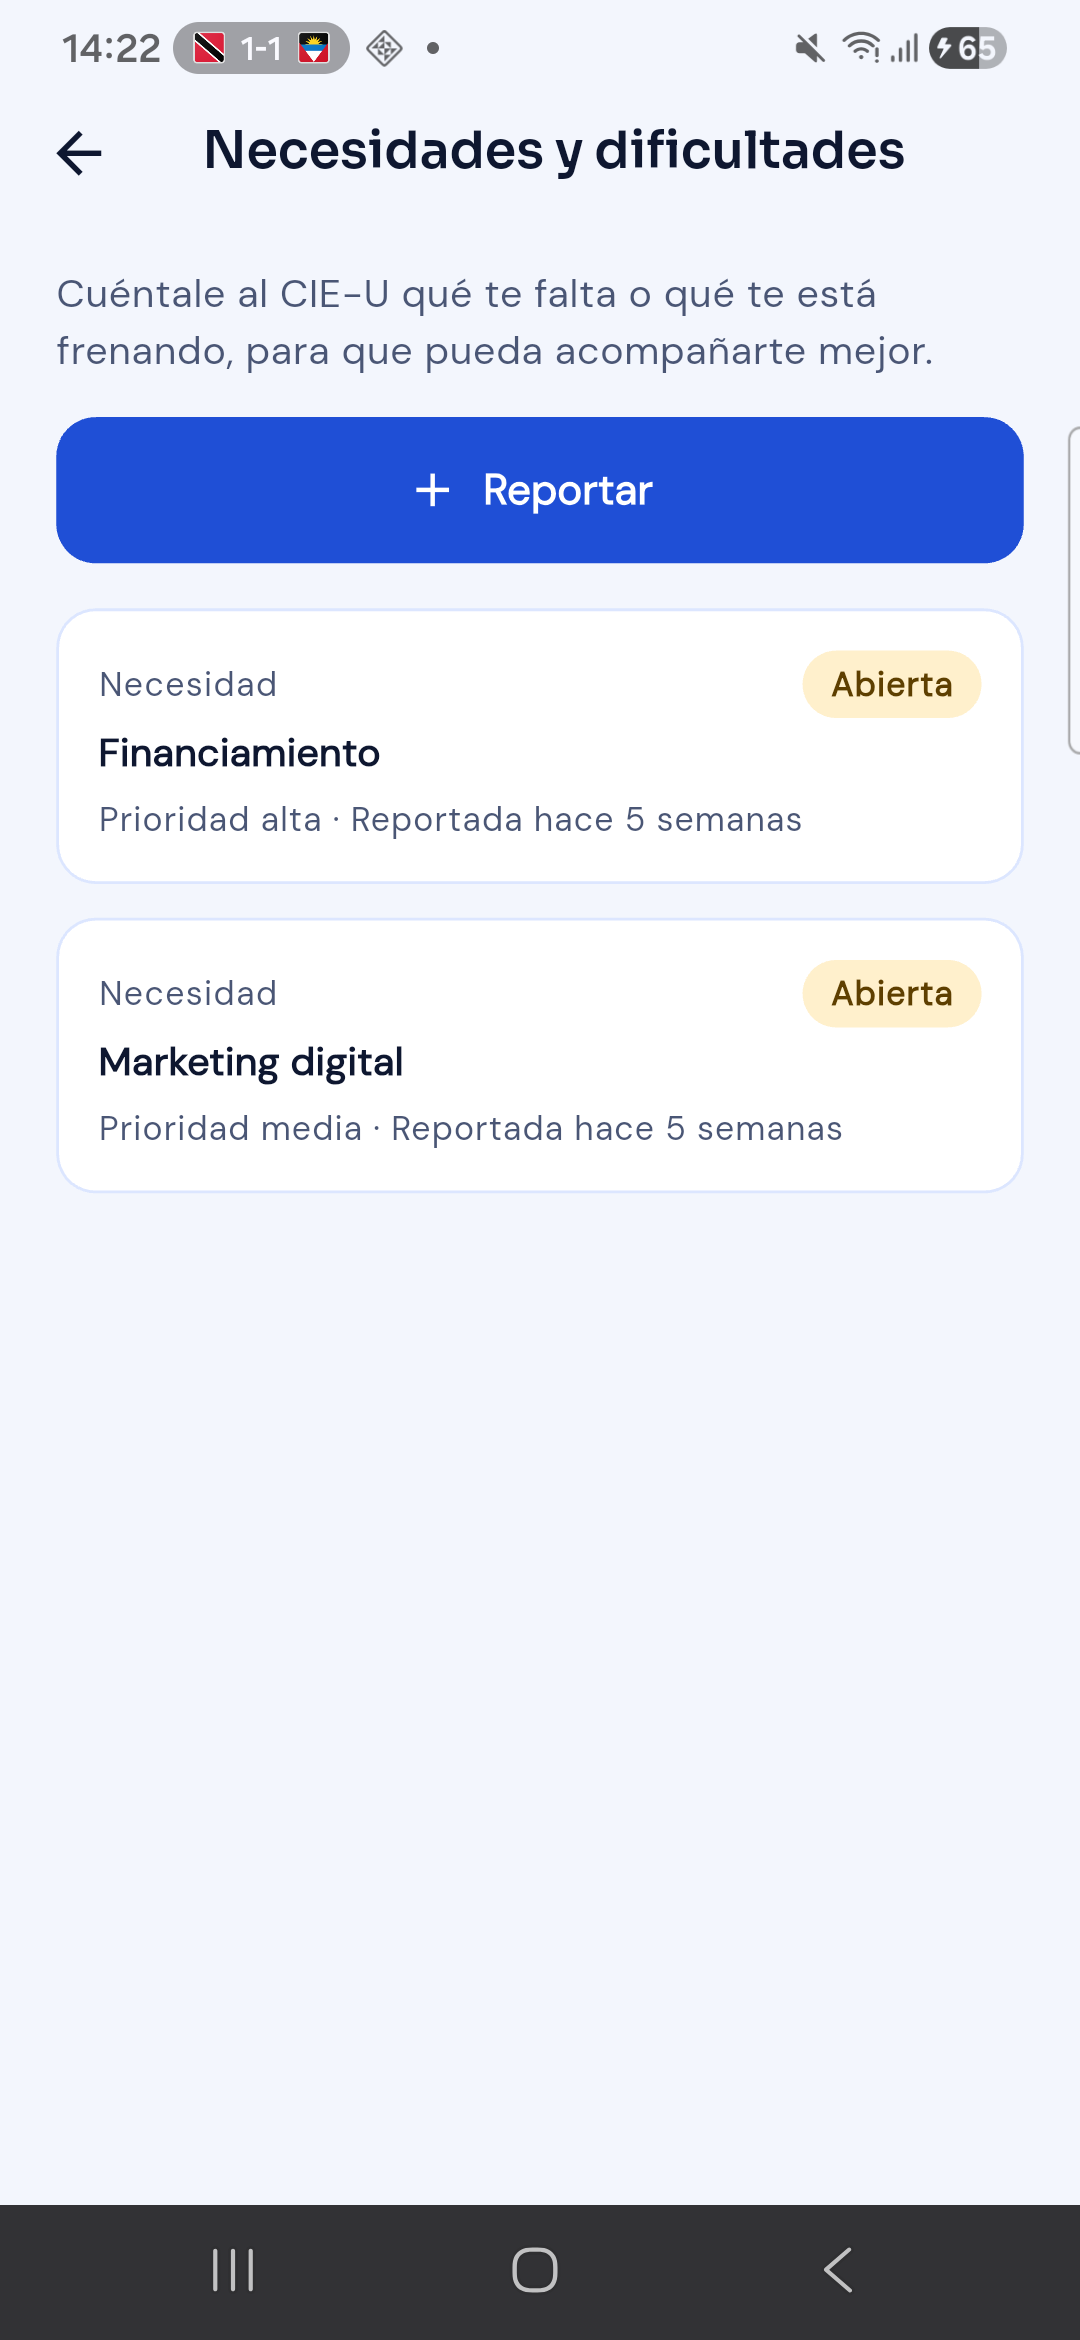
\includegraphics[height=0.52\textheight,keepaspectratio]{imagenes/movil_necesidades.png}}
\par\vspace{3pt}\begin{flushleft}\small \textit{Nota.} Los reportes abiertos se muestran con su prioridad.\end{flushleft}
\end{figure}

No se puede repetir una necesidad abierta: «Ya reportaste esa necesidad y sigue abierta. Cuando se resuelva podrás reportarla otra vez.».

\subsubsection*{5.6.7. Documentos}

\addcontentsline{toc}{subsubsection}{5.6.7. Documentos}

\begin{enumerate}
\item Perfil $\rightarrow$ «Documentos».
\item Tocar «Subir documento» y elegir el archivo.
\item Tocar un documento para abrirlo o descargarlo; el ícono de papelera lo elimina tras confirmar.
\end{enumerate}

\begin{figure}[H]\singlespacing
\caption{Documentos del emprendimiento}\label{fig:movil_documentos}
\centering\fbox{
\includegraphics[height=0.52\textheight,keepaspectratio]{imagenes/movil_documentos.png}}
\par\vspace{3pt}\begin{flushleft}\small \textit{Nota.} Incluye la evidencia de los hitos.\end{flushleft}
\end{figure}

Errores: «Ese tipo de archivo no es válido.», «El archivo es demasiado grande.».

\subsubsection*{5.6.8. Capacitaciones}

\addcontentsline{toc}{subsubsection}{5.6.8. Capacitaciones}

Perfil $\rightarrow$ «Capacitaciones». Lista los talleres y charlas. «Inscribirme» inscribe en las programadas; las etiquetas muestran «Inscrito», «Asististe» o «No asististe».

\begin{figure}[H]\singlespacing
\caption{Capacitaciones}\label{fig:movil_capacitaciones}
\centering\fbox{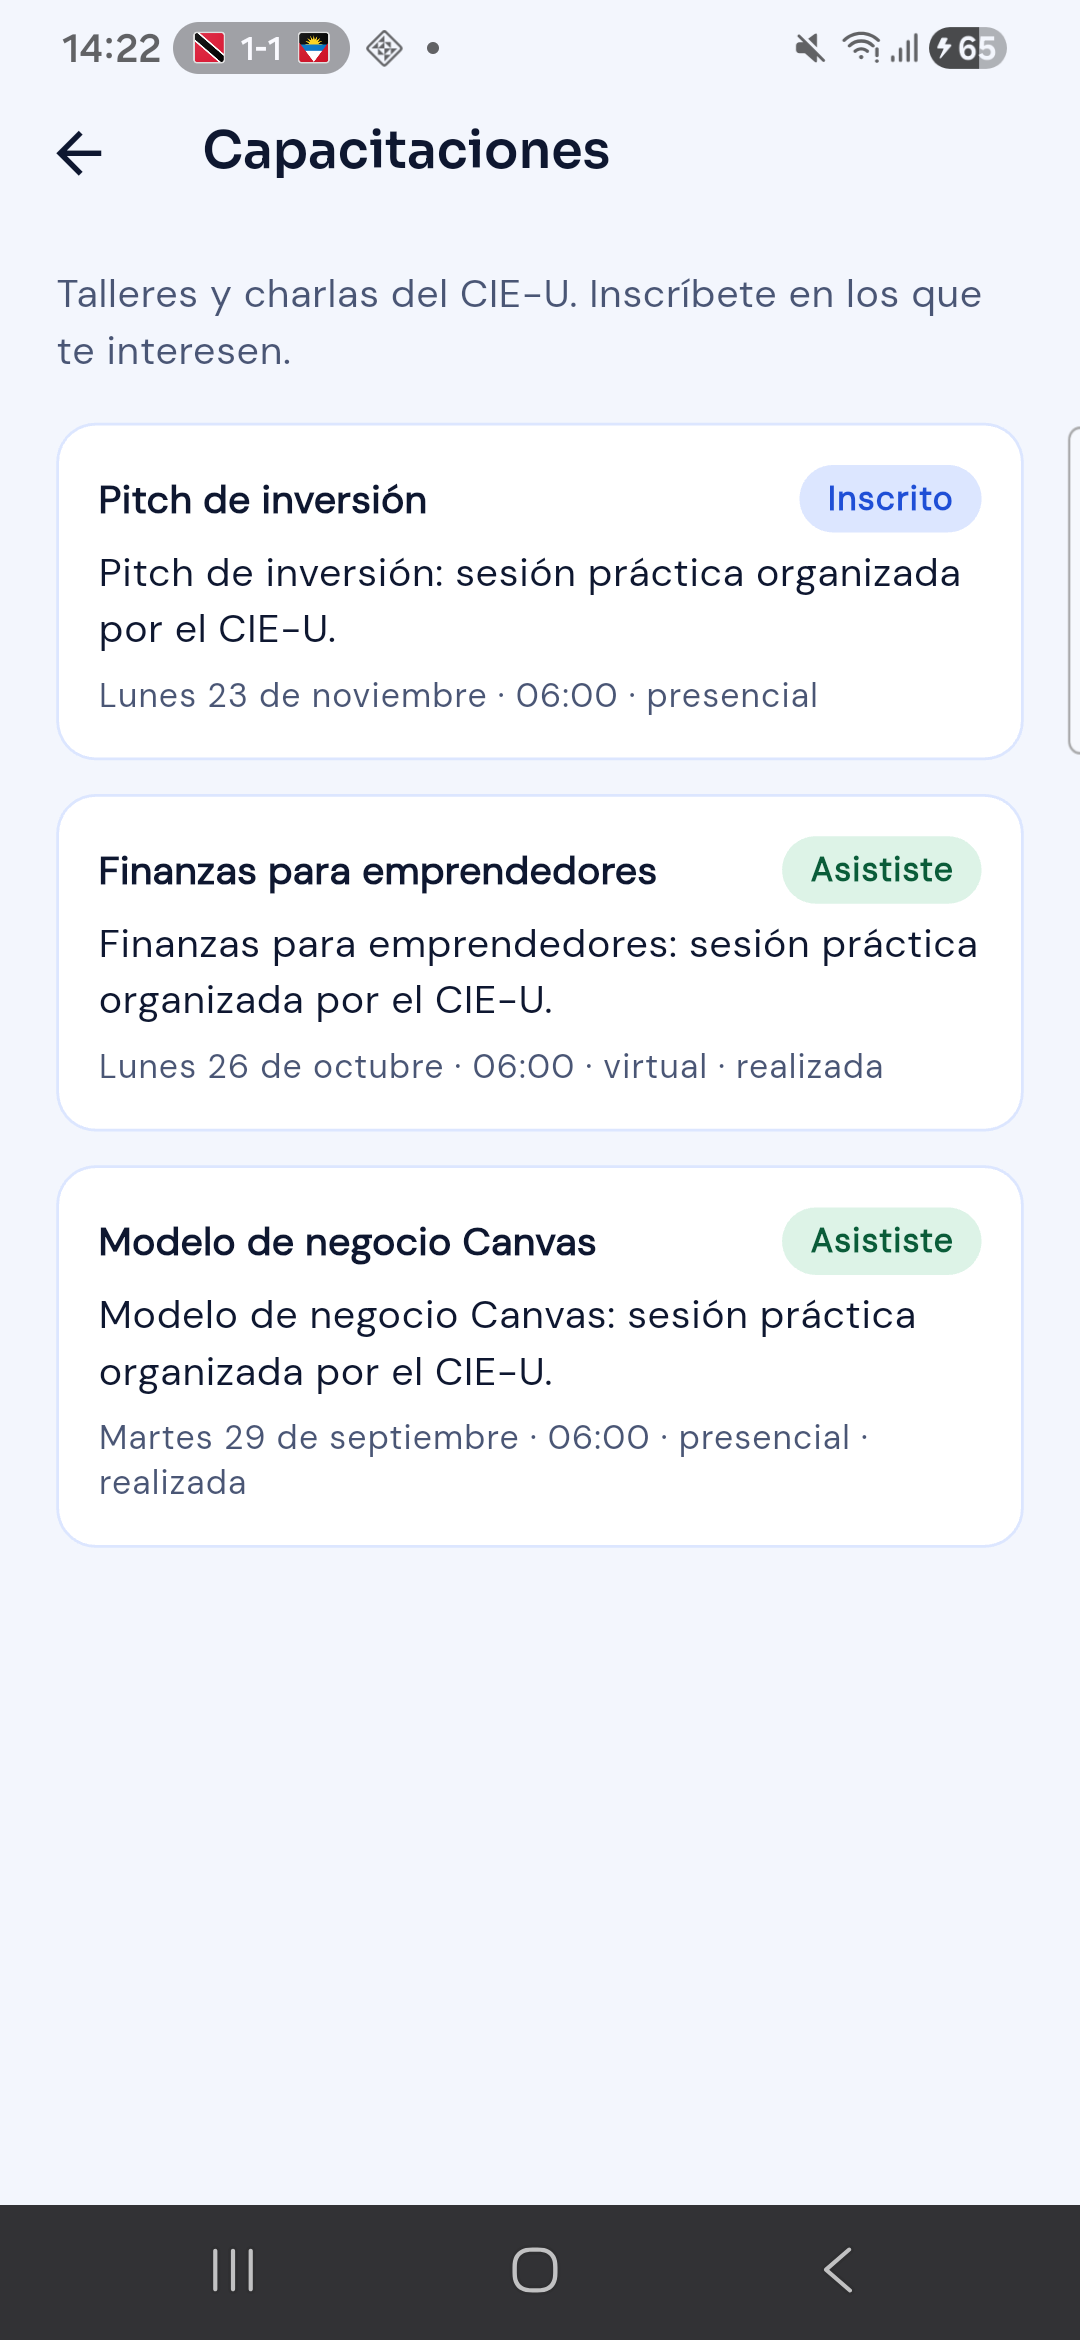
\includegraphics[height=0.52\textheight,keepaspectratio]{imagenes/movil_capacitaciones.png}}
\par\vspace{3pt}\begin{flushleft}\small \textit{Nota.} «Cargar más» muestra más resultados.\end{flushleft}
\end{figure}

\subsubsection*{5.6.9. Notificaciones}

\addcontentsline{toc}{subsubsection}{5.6.9. Notificaciones}

La campana de «Inicio» abre la bandeja «Notificaciones» con avisos de mentorías, compromisos, capacitaciones, etapa e insignias. «Marcar todo leído» limpia los avisos; tocar un aviso abre su pantalla.

\begin{figure}[H]\singlespacing
\caption{Notificaciones}\label{fig:movil_notificaciones}
\centering\fbox{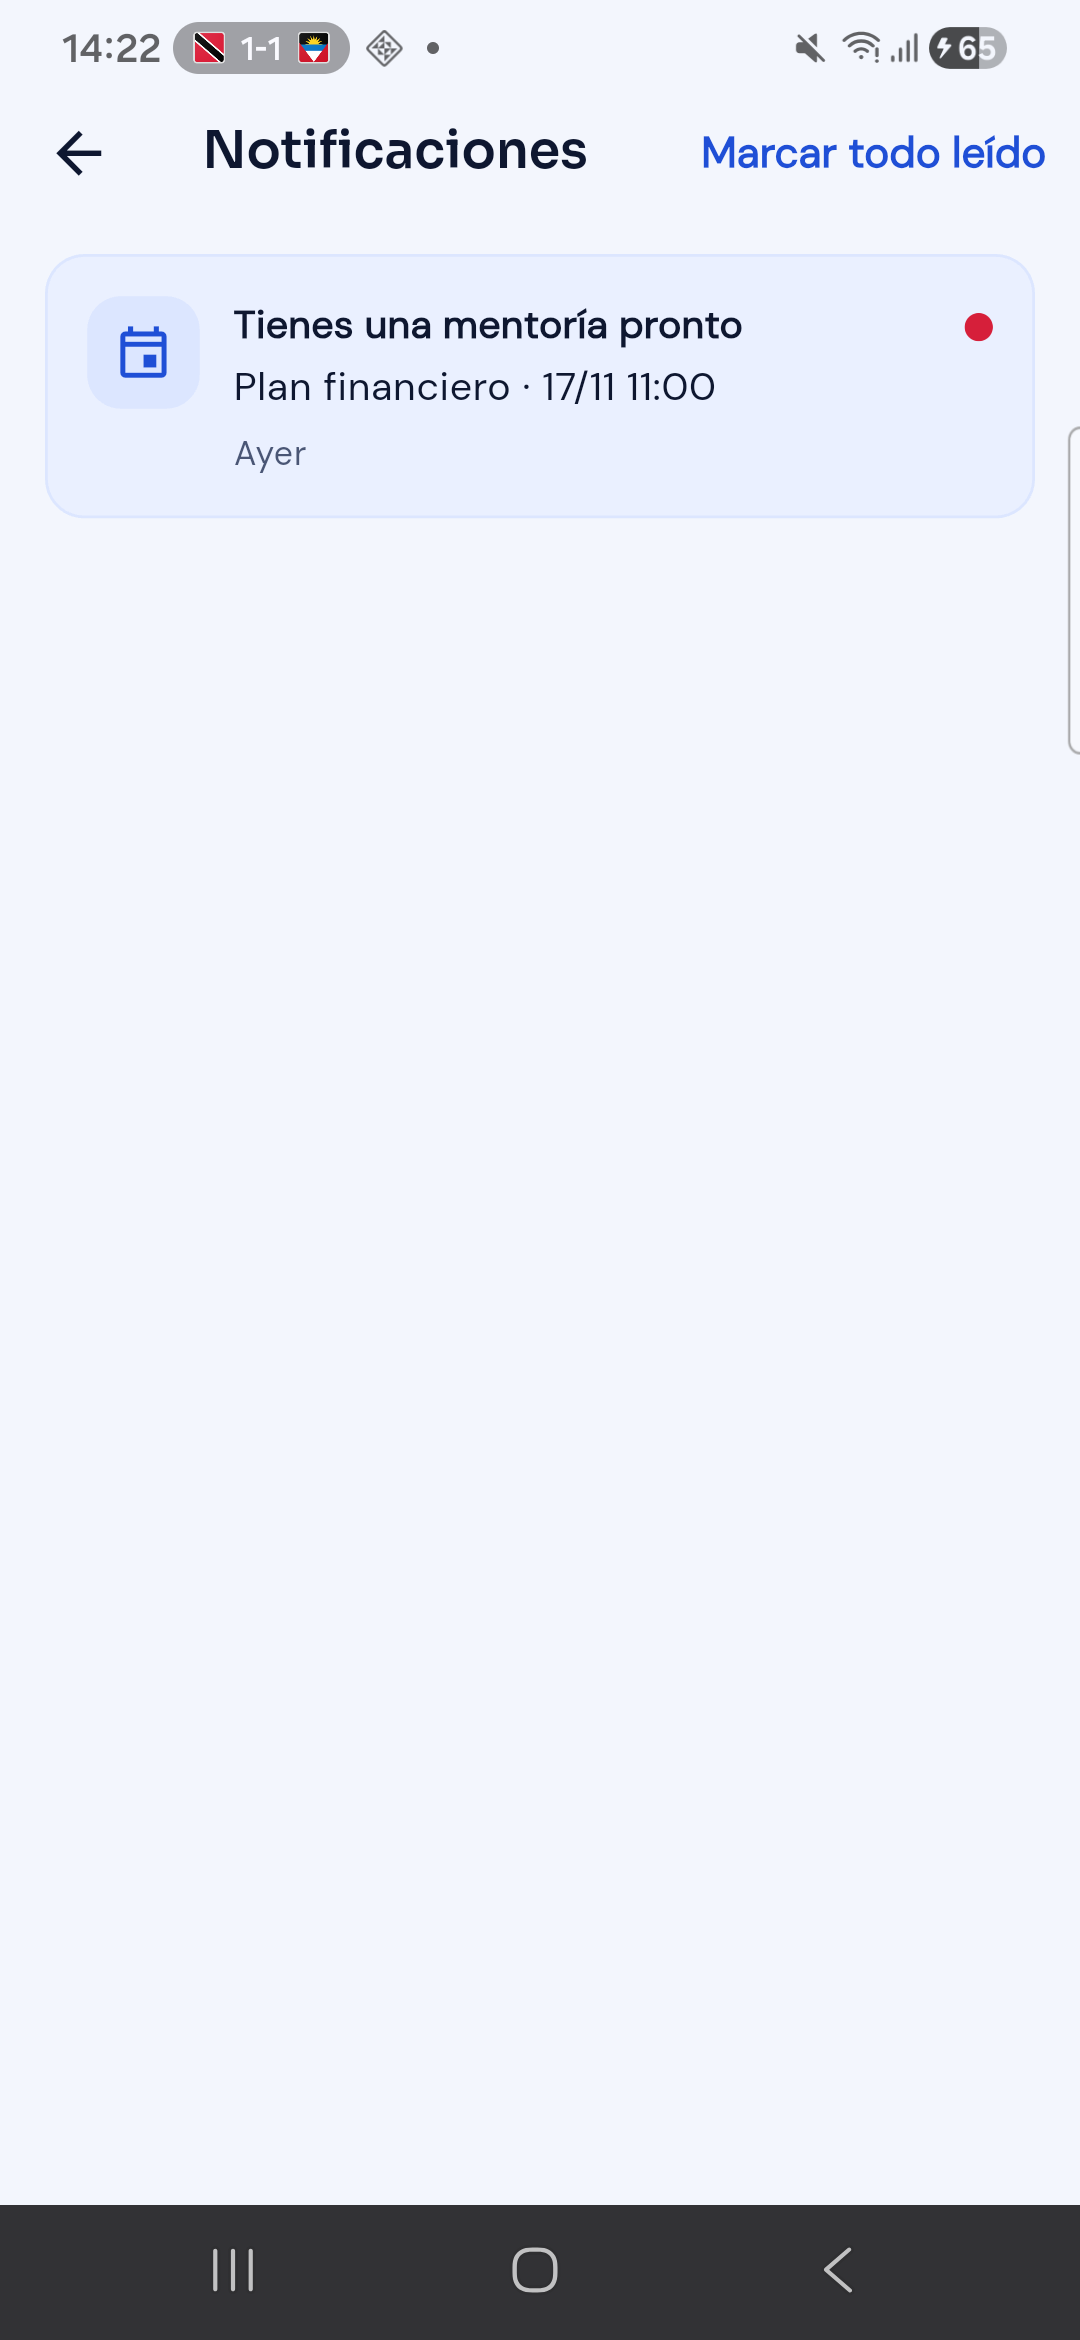
\includegraphics[height=0.52\textheight,keepaspectratio]{imagenes/movil_notificaciones.png}}
\par\vspace{3pt}\begin{flushleft}\small \textit{Nota.} El punto rojo indica un aviso sin leer.\end{flushleft}
\end{figure}

\subsubsection*{5.6.10. Trabajo sin conexión}

\addcontentsline{toc}{subsubsection}{5.6.10. Trabajo sin conexión}

Los compromisos marcados y los avances registrados sin internet se guardan en el teléfono y se envían al recuperar la red («Sincronizando N registro(s)\ldots{}», «Todo sincronizado.»). Las demás funciones requieren conexión.

\clearpage

\section*{CAPÍTULO 6. PROCEDIMIENTOS COMPLETOS}

\addcontentsline{toc}{section}{CAPÍTULO 6. PROCEDIMIENTOS COMPLETOS}

\subsection*{6.1. Admitir una postulación y acompañar al nuevo emprendimiento}

\addcontentsline{toc}{subsection}{6.1. Admitir una postulación y acompañar al nuevo emprendimiento}

\begin{enumerate}
\item La persona postula desde la web pública (sección 3.3).
\item Coordinación abre «Admisiones», revisa y confirma la admisión (5.2.1) y entrega la «Contraseña temporal» a la persona.
\item La persona ingresa a la aplicación móvil (3.2) y cambia su contraseña (5.6.5).
\item Coordinación asigna un asesor al emprendimiento (5.3.1).
\item El asesor define su disponibilidad (5.3.2).
\item La persona agenda su primera mentoría (5.6.3).
\item El asesor registra la sesión, una recomendación y un compromiso (5.3.3).
\item La persona ve el compromiso en «Inicio» y lo marca como cumplido (5.6.1).
\end{enumerate}

\textit{Resultado:} el emprendimiento queda con equipo, asesor, mentorías y compromisos, y su historial lo refleja.

\subsection*{6.2. Avanzar un emprendimiento de etapa}

\addcontentsline{toc}{subsection}{6.2. Avanzar un emprendimiento de etapa}

\begin{enumerate}
\item El emprendedor cumple los retos de la etapa en «Camino» (5.6.2).
\item Coordinación revisa «Progreso» y «Seguimiento» en la ficha (5.2.4).
\item Coordinación usa «Pasar a\ldots{}» y confirma (5.2.3).
\item La pestaña «Etapas» registra el cambio y el emprendedor recibe una notificación.
\end{enumerate}

\subsection*{6.3. Atender una alerta de riesgo}

\addcontentsline{toc}{subsection}{6.3. Atender una alerta de riesgo}

\begin{enumerate}
\item Coordinación o asesor abre «Alertas» y filtra «Abiertas» (5.2.6).
\item Abre la alerta, revisa el motivo y el historial del emprendimiento.
\item Registra el seguimiento: revisada, luego atendida o descartada.
\item Si procede, programa una mentoría o un compromiso (5.3.3).
\end{enumerate}

\subsection*{6.4. Obtener un reporte para la coordinación}

\addcontentsline{toc}{subsection}{6.4. Obtener un reporte para la coordinación}

\begin{enumerate}
\item Abrir «Reportes» y elegir el tipo (5.1.3).
\item Definir periodo y etapa y aplicar.
\item Revisar la vista previa.
\item Seleccionar «Exportar Excel» o «Exportar CSV».
\end{enumerate}

\subsection*{6.5. Recuperar el acceso}

\addcontentsline{toc}{subsection}{6.5. Recuperar el acceso}

Véase la sección 3.4.

\clearpage

\section*{CAPÍTULO 7. MENSAJES Y SOLUCIÓN DE PROBLEMAS}

\addcontentsline{toc}{section}{CAPÍTULO 7. MENSAJES Y SOLUCIÓN DE PROBLEMAS}

\subsection*{7.1. Mensajes informativos}

\addcontentsline{toc}{subsection}{7.1. Mensajes informativos}

\begin{table}[H]\singlespacing\small
\caption{Mensajes informativos frecuentes}
\begin{tabularx}{\textwidth}{XX}
\toprule
\textbf{Mensaje} & \textbf{Dónde aparece} \\
\midrule
\relax Contraseña actualizada. Ya puedes iniciar sesión. & Tras restablecer la contraseña \\
\relax Recibimos tu postulación. El equipo del CIE-U la evaluará\ldots{} & Tras postular \\
\relax Reporte enviado. El CIE-U lo podrá ver. & Aplicación, necesidades \\
\relax Cambios guardados. & Aplicación, editar emprendimiento \\
\relax Mentoría cancelada. & Aplicación, mentorías \\
\relax Todo sincronizado. & Aplicación, sincronización \\
\bottomrule
\end{tabularx}
\end{table}

\subsection*{7.2. Mensajes de advertencia}

\addcontentsline{toc}{subsection}{7.2. Mensajes de advertencia}

\begin{itemize}
\item «Esta decisión es definitiva.» al admitir o rechazar una postulación.
\item «¿Cancelar la mentoría?» y «¿Eliminar «\ldots{}»? No se puede deshacer.»: confirmaciones previas.
\item «Sin conexión. Tus registros se guardan en este dispositivo y se sincronizarán después.»
\end{itemize}

\subsection*{7.3. Errores de validación}

\addcontentsline{toc}{subsection}{7.3. Errores de validación}

\begin{table}[H]\singlespacing\small
\caption{Errores de validación frecuentes}
\begin{tabularx}{\textwidth}{XXX}
\toprule
\textbf{Mensaje} & \textbf{Causa} & \textbf{Solución} \\
\midrule
\relax Ingresa un correo válido. & Formato de correo incorrecto & Escribir un correo completo \\
\relax Usa al menos 8 caracteres. & Contraseña corta & Usar 8 caracteres o más \\
\relax Las contraseñas no coinciden. & La confirmación difiere & Repetir la contraseña igual \\
\relax El código tiene 6 dígitos. & Código incompleto & Escribir los 6 dígitos recibidos \\
\relax Ingresa nombre y apellido. & Nombre de una sola palabra & Escribir nombre y apellido \\
\relax Ese documento ya está registrado. & Documento duplicado & Verificar si el emprendedor ya existe \\
\bottomrule
\end{tabularx}
\end{table}

\subsection*{7.4. Problemas de acceso}

\addcontentsline{toc}{subsection}{7.4. Problemas de acceso}

\begin{table}[H]\singlespacing\small
\caption{Problemas de acceso}
\begin{tabularx}{\textwidth}{XXX}
\toprule
\textbf{Mensaje} & \textbf{Causa} & \textbf{Solución} \\
\midrule
\relax Correo o contraseña incorrectos. & Datos erróneos & Revisar; usar la recuperación de contraseña \\
\relax Tu cuenta está deshabilitada. Contacta al CIE-U. & Cuenta deshabilitada & Contactar a un administrador \\
\relax Esta cuenta es de emprendedor: usa la app móvil del CIE-U. & Emprendedor en el panel web & Usar la aplicación móvil \\
\relax Esta cuenta es del panel web del CIE-U. Esta app es para emprendedores. & Personal en la aplicación & Usar el panel web \\
\relax Tu sesión venció. Ingresa de nuevo. & La sesión dura 60 minutos & Ingresar nuevamente \\
\relax Sin acceso a \ldots{} & Falta el permiso & Pedirlo a un administrador \\
\relax Demasiados intentos. Intenta de nuevo en N min. & Límite de intentos & Esperar el tiempo indicado \\
\bottomrule
\end{tabularx}
\end{table}

\subsection*{7.5. Problemas frecuentes durante el uso}

\addcontentsline{toc}{subsection}{7.5. Problemas frecuentes durante el uso}

\begin{itemize}
\item \textbf{«No se pudo conectar con el servidor. Revisa tu conexión.»:} verificar internet e intentar de nuevo.
\item \textbf{«El servidor tuvo un problema. Intenta de nuevo en unos minutos.»:} esperar y reintentar.
\item \textbf{«El coach no está disponible en este momento.»:} el mensaje no se envió; reintentar más tarde o usar la IA en el celular si está instalada.
\item \textbf{No llega el código de recuperación:} revisar la carpeta de correo no deseado y solicitar un código nuevo.
\item \textbf{No aparece «Agendar mentoría»:} el emprendimiento aún no tiene asesor asignado o habilitado.
\end{itemize}

\subsection*{7.6. Soluciones y recomendaciones}

\addcontentsline{toc}{subsection}{7.6. Soluciones y recomendaciones}

Ante un error persistente, anote el mensaje exacto y la pantalla donde apareció y comuníquese con la coordinación del CIE-U.

\clearpage

\section*{CAPÍTULO 8. BUENAS PRÁCTICAS Y RECOMENDACIONES}

\addcontentsline{toc}{section}{CAPÍTULO 8. BUENAS PRÁCTICAS Y RECOMENDACIONES}

\subsection*{8.1. Uso adecuado del sistema}

\addcontentsline{toc}{subsection}{8.1. Uso adecuado del sistema}

Registre avances y compromisos con frecuencia: el sistema usa esa actividad para calcular la salud del emprendimiento y generar alertas por inactividad.

\subsection*{8.2. Protección de credenciales}

\addcontentsline{toc}{subsection}{8.2. Protección de credenciales}

\begin{itemize}
\item No comparta su contraseña ni su «Contraseña temporal».
\item Cambie la contraseña temporal en el primer ingreso.
\item Use una contraseña de al menos 8 caracteres, distinta de la anterior.
\end{itemize}

\subsection*{8.3. Gestión responsable de la información}

\addcontentsline{toc}{subsection}{8.3. Gestión responsable de la información}

Suba solo documentos del emprendimiento. Los archivos que se agregan al coach desde «Mis archivos para la IA» se analizan únicamente en el teléfono y se borran al cerrar sesión. Los datos de postulantes y emprendedores deben tratarse con confidencialidad.

\subsection*{8.4. Recomendaciones para evitar errores}

\addcontentsline{toc}{subsection}{8.4. Recomendaciones para evitar errores}

\begin{itemize}
\item Revise los datos antes de confirmar acciones definitivas.
\item Confirme que el asesor esté habilitado antes de asignarlo.
\item Use Wi-Fi para descargar la IA en el teléfono.
\end{itemize}

\subsection*{8.5. Consideraciones de seguridad aplicables al usuario}

\addcontentsline{toc}{subsection}{8.5. Consideraciones de seguridad aplicables al usuario}

Cierre la sesión en equipos compartidos. Al cambiar la contraseña, las demás sesiones se cierran automáticamente. Las acciones sensibles del personal quedan registradas en «Auditoría».

\clearpage

\section*{CAPÍTULO 9. GLOSARIO DE TÉRMINOS}

\addcontentsline{toc}{section}{CAPÍTULO 9. GLOSARIO DE TÉRMINOS}

\begin{table}[H]\singlespacing\small
\caption{Glosario}
\begin{tabularx}{\textwidth}{XX}
\toprule
\textbf{Término} & \textbf{Definición} \\
\midrule
\relax CIE-U & Centro de Innovación y Emprendimiento Universitario. \\
\relax Emprendimiento & Proyecto de negocio acompañado por el programa. \\
\relax Etapa & Fase del programa: Preincubación, Incubación, Crecimiento o Graduación. \\
\relax Reto & Tarea de una etapa que otorga XP al cumplirse. \\
\relax XP & Puntos de experiencia que acumula el emprendedor. \\
\relax Insignia & Reconocimiento por logros del programa. \\
\relax Compromiso & Tarea acordada en una mentoría, con responsable y fecha. \\
\relax Recomendación & Sugerencia que registra el asesor tras una sesión. \\
\relax Hito & Logro del emprendimiento que se registra, con evidencia opcional. \\
\relax Alerta & Aviso de riesgo detectado por el sistema. \\
\relax Coach IA & Asistente de inteligencia artificial que responde con la base de conocimiento del CIE-U. \\
\relax Contraseña temporal & Clave inicial mostrada una sola vez al crear una cuenta. \\
\relax Auditoría & Registro de las acciones sensibles realizadas. \\
\bottomrule
\end{tabularx}
\end{table}

\clearpage

\section*{CAPÍTULO 10. PREGUNTAS FRECUENTES}

\addcontentsline{toc}{section}{CAPÍTULO 10. PREGUNTAS FRECUENTES}

\textbf{¿Puede un emprendedor entrar al panel web?} No. Debe usar la aplicación móvil.

\textbf{¿Quién crea las cuentas del personal?} Un administrador, desde «Usuarios».

\textbf{¿Qué pasa si olvido mi contraseña?} Use «¿Olvidaste tu contraseña?» y el código de 6 dígitos enviado por correo; vence en 15 minutos.

\textbf{¿Puedo usar el coach sin internet?} Sí, si descargó la IA desde Perfil $\rightarrow$ «IA en tu celular». Los archivos propios no salen del teléfono.

\textbf{¿Por qué no puedo agendar una mentoría?} Porque no tiene asesor asignado o el asesor no tiene horarios disponibles.

\textbf{¿Puedo deshacer la admisión de una postulación?} No, la decisión es definitiva.

\textbf{¿Qué formatos de reporte existen?} CSV y Excel para los reportes; CSV para la auditoría.

\textbf{¿Qué ocurre si registro un avance sin conexión?} Queda guardado en el teléfono con la etiqueta «Pendiente de sincronizar» y se envía al volver la red.

\clearpage

\section*{REFERENCIAS}

Este manual se basa en la inspección directa del sistema y no cita fuentes externas. Su formato adapta las pautas de presentación del siguiente documento:

\begin{hangref}American Psychological Association. (2020). \textit{Publication manual of the American Psychological Association} (7.ª ed.). American Psychological Association.\end{hangref}

\clearpage

\clearpage

\section*{ANEXOS}

\subsection*{Anexo A. Pantallas adicionales por rol}

\addcontentsline{toc}{subsection}{Anexo A. Pantallas adicionales por rol}

\begin{figure}[H]\singlespacing
\caption{Resumen del coordinador}\label{fig:web_coordinador_panel}
\centering\fbox{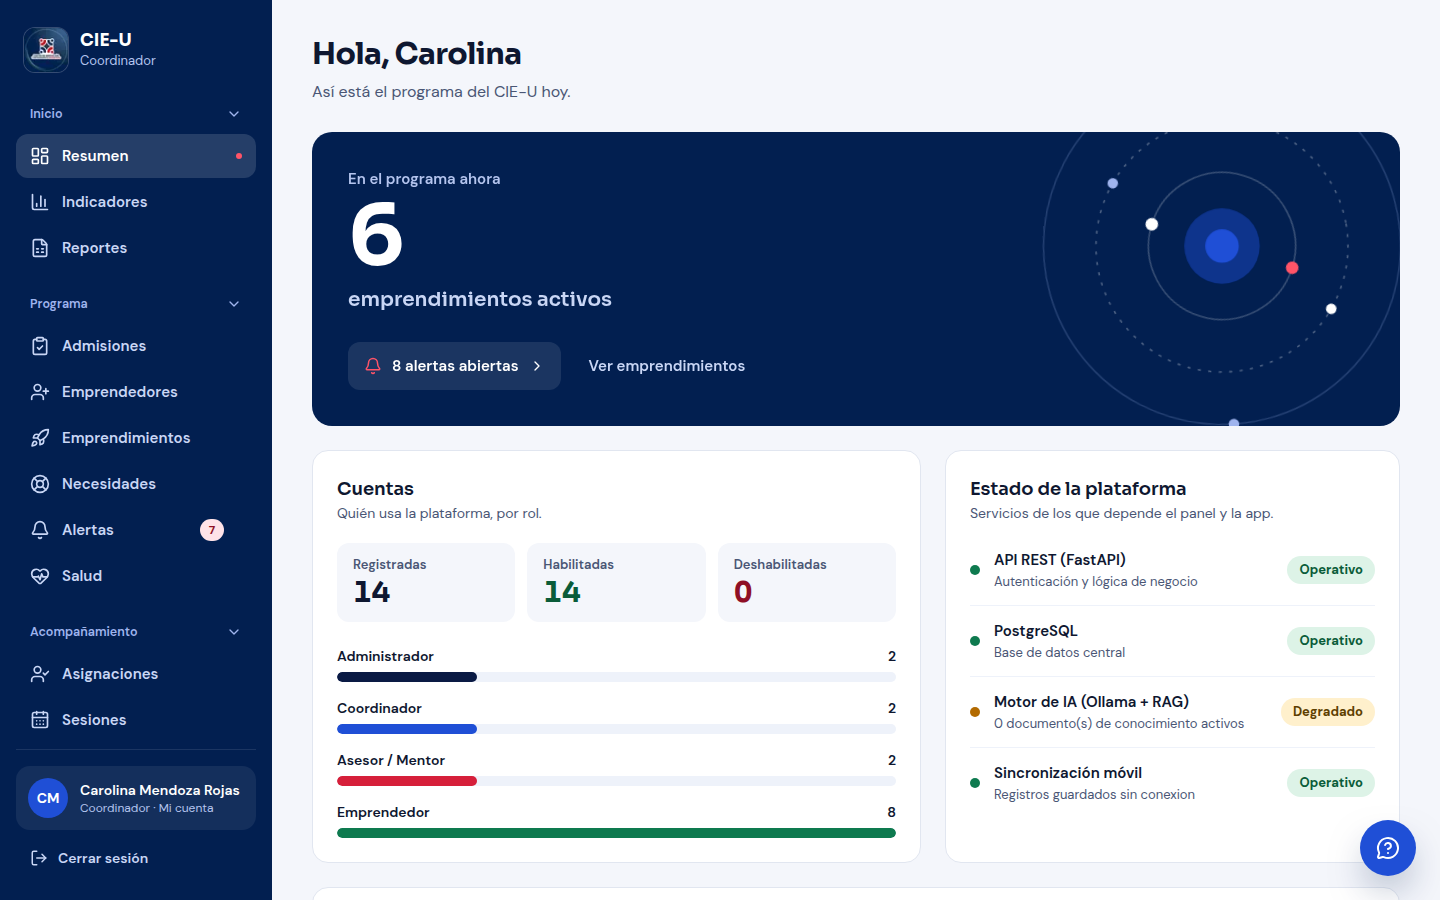
\includegraphics[width=0.97\textwidth,keepaspectratio]{imagenes/web_coordinador_panel.png}}
\par\vspace{3pt}\begin{flushleft}\small \textit{Nota.} Vista inicial con el rol Coordinador.\end{flushleft}
\end{figure}

\begin{figure}[H]\singlespacing
\caption{Alertas vistas por un asesor}\label{fig:web_asesor_alerts}
\centering\fbox{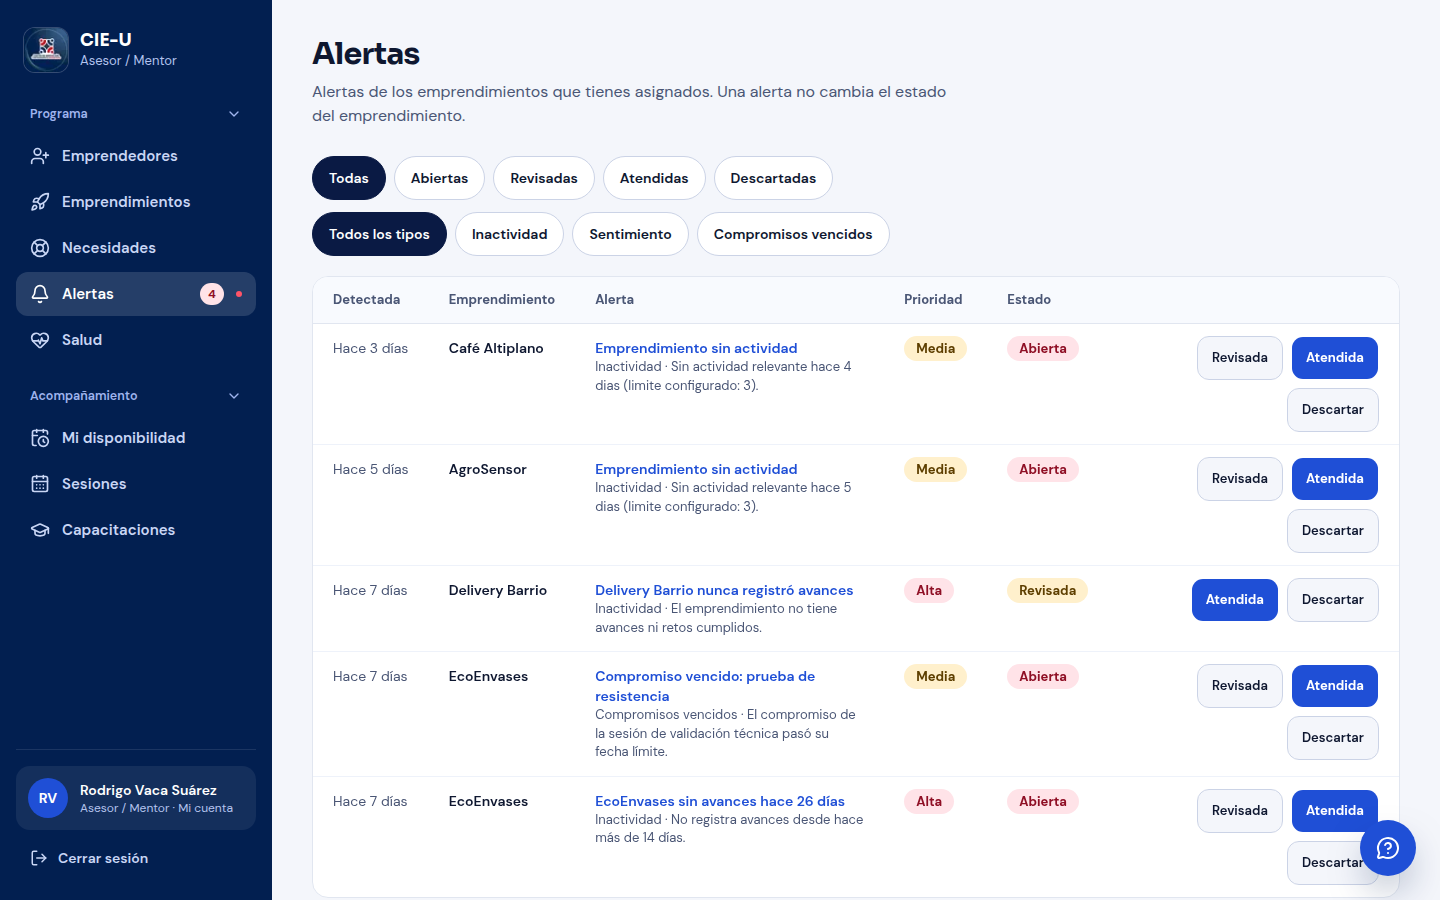
\includegraphics[width=0.97\textwidth,keepaspectratio]{imagenes/web_asesor_alerts.png}}
\par\vspace{3pt}\begin{flushleft}\small \textit{Nota.} El asesor ve solo las alertas de sus emprendimientos.\end{flushleft}
\end{figure}

\begin{figure}[H]\singlespacing
\caption{Restablecimiento de contraseña}\label{fig:web_reset}
\centering\fbox{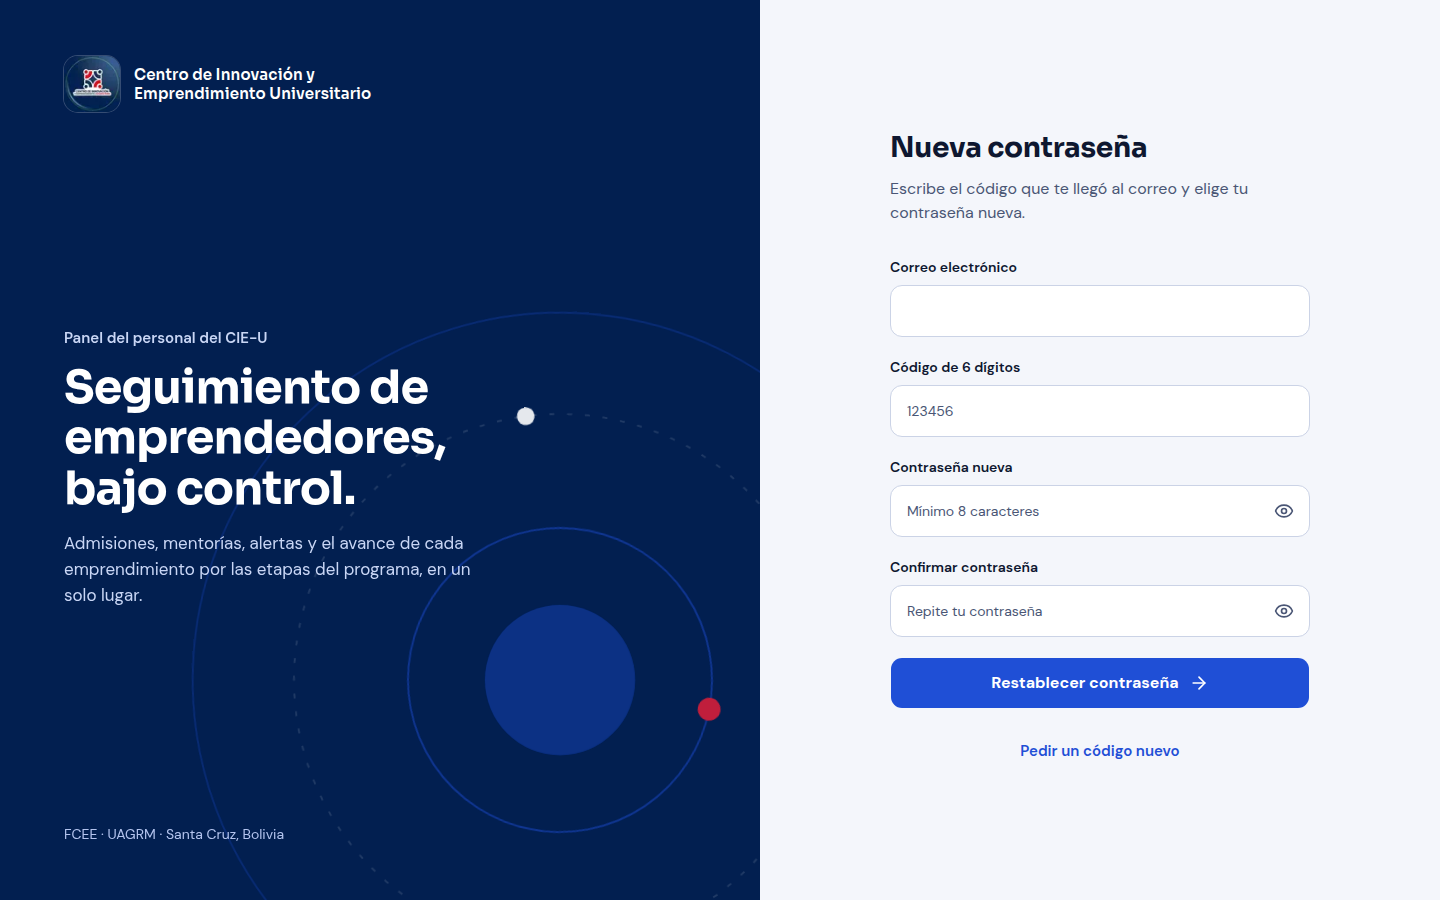
\includegraphics[width=0.97\textwidth,keepaspectratio]{imagenes/web_reset.png}}
\par\vspace{3pt}\begin{flushleft}\small \textit{Nota.} Pantalla para escribir el código y la nueva contraseña.\end{flushleft}
\end{figure}

\subsection*{Anexo B. Capturas y verificaciones pendientes}

\addcontentsline{toc}{subsection}{Anexo B. Capturas y verificaciones pendientes}

\begin{table}[H]\singlespacing\small
\caption{Elementos pendientes de verificar}
\begin{tabularx}{\textwidth}{XX}
\toprule
\textbf{Elemento} & \textbf{Estado} \\
\midrule
\relax [CAPTURA PENDIENTE: registro y recuperación de contraseña en la aplicación móvil] & No capturadas; el procedimiento se basa en el código \\
\relax [CAPTURA PENDIENTE: formularios en hoja lateral del panel web (nuevo usuario, nuevo emprendimiento, registrar sesión)] & No capturadas \\
\relax [CAPTURA PENDIENTE: Coach IA con respuesta y fuentes] & No verificado: el servicio de IA estaba desactivado \\
\relax Envío de correos de recuperación y notificaciones push & No verificado en el entorno de prueba \\
\relax Exportaciones CSV/Excel & Presentes en la interfaz; descarga no abierta \\
\bottomrule
\end{tabularx}
\end{table}

La lista completa está en el archivo \texttt{pendientes\_verificacion.md}.

\end{document}